\documentclass[11pt,letterpaper]{article}

% --- Packages ---
\usepackage[utf8]{inputenc}
\usepackage[T1]{fontenc}
\usepackage{lmodern}
\usepackage{microtype}
\usepackage[margin=1in]{geometry}
\usepackage{amsmath,amssymb,amsfonts,amsthm}
\usepackage{mathtools}
\usepackage{booktabs}
\usepackage{array}
\usepackage{multirow}
\usepackage{caption}
\usepackage{graphicx}
\usepackage{xcolor}
\usepackage{xurl}
\usepackage[colorlinks=true,linkcolor=blue!60!black,citecolor=blue!60!black,urlcolor=blue!60!black]{hyperref}

% --- Float Placement ---
\renewcommand{\topfraction}{0.85}
\renewcommand{\bottomfraction}{0.70}
\renewcommand{\textfraction}{0.10}
\renewcommand{\floatpagefraction}{0.75}

% --- Theorem Environments ---
\theoremstyle{plain}
\newtheorem{theorem}{Theorem}
\newtheorem{proposition}{Proposition}
\newtheorem{corollary}{Corollary}

\theoremstyle{definition}
\newtheorem{definition}{Definition}

\theoremstyle{remark}
\newtheorem{remark}{Remark}

% --- Custom Macros ---
\newcommand{\WAR}{\mathrm{WAR}}
\newcommand{\WAA}{\mathrm{WAA}}
\newcommand{\PA}{\mathrm{PA}}
\newcommand{\BF}{\mathrm{BF}}
\newcommand{\IP}{\mathrm{IP}}
\newcommand{\JAWS}{\mathrm{JAWS}}
\newcommand{\SJAWS}{\mathrm{S\text{-}JAWS}}
\newcommand{\RJAWS}{\mathrm{R\text{-}JAWS}}
\newcommand{\ZWAR}{Z_{\WAR}}
\newcommand{\Zpos}{Z_{\mathrm{pos}}}
\newcommand{\Zpitch}{Z_{\mathrm{pitch}}}
\newcommand{\Zpool}{Z_{\mathrm{pool}}}
\newcommand{\Ztwoway}{Z_{\mathrm{2D}}}
\newcommand{\SE}{\mathrm{SE}}
\newcommand{\SD}{\mathrm{SD}}
\newcommand{\Var}{\mathrm{Var}}
\newcommand{\E}{\mathbb{E}}
\newcommand{\DKL}{D_{\mathrm{KL}}}
\newcommand{\R}{\mathbb{R}}
\newcommand{\N}{\mathcal{N}}
\newcommand{\sgn}{\operatorname{sgn}}
\newcommand{\Ical}{\mathcal{I}}

% --- Title & Author ---
\title{\textbf{From Total WAR to WAR Rate:\\
The $\alpha$-Family and the Empirical Case for $\alpha \approx 1/5$}}

\author{
  Will Findley\\
  \texttt{findley@gmail.com}
}

\date{October 23, 2026}

\begin{document}

\maketitle

\begin{abstract}
\noindent
Ranking careers of unequal length requires trading cumulative value against rate. We study the one-parameter family $Z_\alpha = \WAR/N^{\alpha}$, where $N$ counts plate appearances for hitters and batters faced for pitchers, which spans career $\WAR$ ($\alpha = 0$) and the $\WAR$ rate ($\alpha = 1$). The exponent has a direct meaning: extra playing time raises $Z_\alpha$ only if its rate exceeds $\alpha$ times the career rate. Which exponent is right depends on how the quantity being tracked scales with rate and exposure. Two members have a theoretical claim. $Z_{1/2}$ is $\sigma$ times a career's signal-to-noise ratio against replacement level and the only member that scores every career with equal precision, which makes $\alpha = \tfrac12$ the natural hypothesis for the most predictive exponent. If a season worth $s$ $\WAR$ is worth $s^{\gamma}$, constant-rate careers of common season length are ranked by total value at $\alpha = 1 - 1/\gamma$; win--pennant curves fitted to $2{,}622$ team-seasons give $\gamma \approx 1.17$--$1.30$, or $\alpha \approx 0.14$--$0.23$. We test both against $42$ benchmarks: Hall of Fame election, two expert top-100 lists, All-Star and award honors, and forecasts of future $\WAR$, honors and election. The data reject the $z$-statistic hypothesis: $\alpha = \tfrac15$ scores at least as well as $\alpha = \tfrac12$ on $35$ benchmarks, significantly better on $20$, and significantly worse on none. Judgments of finished careers peak at $\alpha \approx 0.20$--$0.30$, next to the pennant-race range, and $Z_{1/5}$ matches or beats career $\WAR$ and $\JAWS$ in Hall of Fame classification in seven of eight pools. Forecasts of cumulative outcomes favor career $\WAR$ itself (against which $\alpha = \tfrac15$ is significantly better on $5$ benchmarks and worse on $12$), consistent with playing time persisting more than rate. No single exponent is optimal for every target, but $\alpha = \tfrac15$ comes within $0.001$ of the smallest worst-case and average shortfall from each benchmark's own optimum (attained at $0.10$--$0.15$). At $\alpha = \tfrac15$, Babe Ruth ranks first, Walter Johnson and Cy Young fifth and seventh, and the all-time top 100 contains as many pitchers as the expert lists.
\end{abstract}

\vspace{0.5em}
\noindent\textbf{Keywords:} Sabermetrics, Wins Above Replacement, Career Valuation, Batters Faced, Pennants Added, Hall of Fame, Forecasting, JAWS

\section{Introduction}

Every career evaluation framework in baseball must handle two problems. The first is the trade-off between \emph{cumulative volume} (total Wins Above Replacement, $W = \WAR$) and \emph{per-opportunity rate} ($\bar r = \WAR / N$, with $N$ the number of plate appearances or batters faced). The second is placing position players, starting pitchers and relief pitchers on one scale. Ranking by $W$ alone favors long careers at modest rates and buries relievers. Ranking by $\bar r$ alone favors brief call-ups.

Three families of compromise are in common use:

\begin{enumerate}
    \item \textbf{Peak-window averages ($\JAWS$, $\SJAWS$, $\RJAWS$).} Jaffe's $\JAWS$ \cite{jaffe2004,jaffe2017} averages career $\WAR$ with $\WAR_7$, the sum of a player's seven best seasons:
    \begin{equation}
        \JAWS = \frac{\WAR + \WAR_7}{2}.
    \end{equation}
    The window length ($k=7$) and the equal weight are design choices, and the season is the unit of opportunity. Season-based peaks therefore favor 19th- and early-20th-century starters, who often faced $1{,}400$--$2{,}500$ batters per season against $650$--$850$ for modern starters. Starter JAWS ($\SJAWS$) \cite{jaffe2022} prorates peak seasons above $250\,\IP$ down to $250\,\IP$, leaving the career half unadjusted. For relievers, Baseball-Reference's Reliever JAWS ($\RJAWS$) is the average of career $\WAR$, Win Probability Added ($\mathrm{WPA}$) and context-neutral $\mathrm{WPA/LI}$ \cite{bbrefjawsrp}. This works well within the reliever pool but leaves the $\WAR$ scale, so relievers cannot be compared directly with starters.

    \item \textbf{Shifted baselines ($\WAA$).} Wins Above Average moves the reference rate from replacement level to league average ($r_{\mathrm{avg}} \approx 2.0\,\WAR$ per $650\,\PA$):
    \begin{equation}
        \WAA = \WAR - r_{\mathrm{avg}} N.
    \end{equation}
    $\WAA$ therefore lowers a player's score for any season below average, including seasons above replacement level, a deliberate choice that emphasizes peak value.

    \item \textbf{Shrunken rates.} Adding $N_0$ pseudo-opportunities at a prior rate $r_0$ gives an estimate of true talent \cite{efron1975,tango2007,albert2017}:
    \begin{equation}
        \hat{r}_{\mathrm{EB}} = \frac{\WAR + N_0 r_0}{N + N_0}.
    \end{equation}
    This is the right tool for estimating talent. For full careers ($N \gg N_0$), however, it converges to the raw rate and does not reward durability.
\end{enumerate}

\paragraph{The $\alpha$-family.} This paper studies a fourth compromise, the one-parameter family
\begin{equation*}
    Z_\alpha = \frac{\WAR}{N^{\alpha}}, \qquad 0 \le \alpha \le 1,
\end{equation*}
with $N$ counted in events (plate appearances or batters faced, one for one). It runs continuously from career $\WAR$ ($\alpha = 0$) to the $\WAR$ rate ($\alpha = 1$), and every interior member is a weighted geometric mean of the two. The question is what the exponent should be. Our thesis has three parts.
\begin{enumerate}
    \item[(1)] \emph{The natural theoretical answer, $\alpha = \tfrac12$, is wrong.} $Z_{1/2} = \WAR/\sqrt N$ is $\sigma$ times the $z$-statistic of a career's record against replacement level, its estimated signal-to-noise ratio, and it is the only member of the family whose sampling noise is the same for every career. That makes it the obvious hypothesis for the most predictive exponent, and this work began from it. Across $42$ benchmarks it is never significantly better than $\alpha = \tfrac15$ and is significantly worse on $20$; where it comes closest (hitter forecasts, relievers), its advantage over $\tfrac15$ is a few thousandths.
    \item[(2)] \emph{The value of a great season explains the data.} If a season worth $s$ $\WAR$ is worth $s^{\gamma}$, ranking careers by total value corresponds to $\alpha = 1 - 1/\gamma$. Pennant races, which involve no judgment about players, put $\gamma$ near $1.25$, i.e.\ $\alpha \approx \tfrac15$: a $10$-$\WAR$ season is worth about two and a half $5$-$\WAR$ seasons, not the four that $\alpha = \tfrac12$ implies. Hall of Fame voting and expert rankings peak nearby, at $0.20$--$0.30$, and their regret is smallest at exactly $\alpha = 0.20$.
    \item[(3)] \emph{$\alpha \approx \tfrac15$ is the best single exponent, although not the best for every target.} Forecasts of future totals reward playing time more than value judgments do: most are best predicted by career $\WAR$ itself, which beats $\alpha = \tfrac15$ significantly on $12$ of the $42$ benchmarks (and loses significantly on $5$). Forecasts of future rates reward playing time less. A simple scaling result (Proposition~\ref{prop:target}) suggests why. Across all benchmarks, the worst-case and the average shortfall from each benchmark's own optimum are smallest at $0.10$--$0.15$; $\alpha = \tfrac15$ is within $0.001$ of both minima, whereas $\alpha = \tfrac12$ is far from them.
\end{enumerate}

\paragraph{Contributions.}
\begin{itemize}
    \item[(i)] \emph{An interpretable dial.} Additional playing time raises $Z_\alpha$ if and only if its marginal rate exceeds $\alpha$ times the career rate (Proposition~\ref{prop:alpha}). A target that scales as $\bar r^{\,a} N^{b}$ is ranked exactly by $Z_\alpha$ with $\alpha = 1 - b/a$ (Proposition~\ref{prop:target}), which places career $\WAR$, the rate, the $z$-statistic, season value and forecasts on one map.
    \item[(ii)] \emph{Two derived exponents.} The $z$-statistic member $\alpha = \tfrac12$ (Proposition~\ref{prop:frequentist}), and the value member $\alpha = 1 - 1/\gamma$ (Proposition~\ref{prop:gamma}) with $\gamma$ estimated from $2{,}622$ team-seasons of pennant races (Section~\ref{sec:gamma}).
    \item[(iii)] \emph{A broad empirical test.} Hall of Fame election in eight pools, two expert lists, All-Star and award honors, and checkpoint and midpoint forecasts of future $\WAR$, honors and election, with bootstrap intervals for every optimal exponent (Section~\ref{sec:convergence}).
    \item[(iv)] \emph{One scale for all roles.} Per-event noise is nearly the same for hitters, starters and relievers, which justifies counting one plate appearance as one batter faced; a value-consistent $\ell_\gamma$ rule combines the two coordinates of two-way players and reduces to total $\WAR$ at $\alpha = 0$ (Section~\ref{sec:twoway_theory}).
    \item[(v)] \emph{Leaderboards at $\alpha = \tfrac15$} for hitters, starters, relievers, two-way players and all players together, with career-$\WAR$ and $Z_{1/2}$ ranks for comparison (Section~\ref{sec:empirical}).
\end{itemize}
Every modeling choice is listed in Table~\ref{tab:choices}.

\section{Related Work}
\label{sec:related}

\paragraph{JAWS and its variants.} $\JAWS$ \cite{jaffe2004,jaffe2017} is the most widely cited Hall of Fame benchmark. $\SJAWS$ \cite{jaffe2022} adjusts the peak component for heavy early-era workloads, and Baseball-Reference's Reliever JAWS ($\RJAWS$) \cite{bbrefjawsrp} averages $\WAR$ with two win-probability measures for relievers.

\paragraph{Hall Rating.} Darowski's Hall of Stats \cite{hallofstats} combines adjusted $\WAR$ and $\WAA$ and scales the result so that $100$ marks the Hall of Fame borderline. Like $Z_\alpha$, it mixes a volume measure with a rate-sensitive measure; unlike $Z_\alpha$, it does so through a weighted sum.

\paragraph{Opportunity-standardized peaks.} Gordon's Standardized Peak WAR (SPW) \cite{gordon2023} is the closest precedent for our choice of exposure units. It replaces the season as the unit of a peak window with a fixed amount of opportunity, $\PA$ for hitters and $\BF$ for pitchers, by accumulating a player's highest-rate seasons until a standard exposure is reached, so that early-era workhorses, modern starters and relievers can be compared. The family $Z_\alpha$ shares the $\PA$/$\BF$ exposure units but differs in three ways: it is a career-level statistic computed from totals $(W, N)$ rather than from a selected subset of seasons; it has a single parameter $\alpha$ with the marginal-rate interpretation of Proposition~\ref{prop:alpha}; and it places hitters and pitchers on one scale through $\PA \equiv \BF$.

\paragraph{Nonlinear seasonal value.} Jaffe justifies $\JAWS$'s effective double counting of peak seasons by appeal to ``research into pennants added and the premium value of star talent,'' since individual greatness can have a non-linear effect on team results \cite{jaffe2017si}. That line of work, which goes back to Bill James's proposal in \emph{The Politics of Glory} \cite{james1994} and was implemented by Wolverton \cite{wolverton2002}, Levitt \cite{levitt2004} and Gassko \cite{gassko2007}, maps each season's value into a nonlinear contribution to playoff, pennant or championship probability at the cost of a season-level model (Gassko~\cite{gassko2007} found that wild-card playoff odds flatten at high $\WAR$ and favor longevity, consistent with our nearly linear postseason-berth estimate in Table~\ref{tab:gamma}, whereas pennants and championships remain convex). We do not propose a new pennants-added measure. Our contribution is to summarize the win--pennant curve by a single power-law exponent $\gamma$ and to show that, for constant-rate careers with a common season length, it fixes the exponent of a career-total statistic, $\alpha = 1 - 1/\gamma$ (Proposition~\ref{prop:gamma}, Section~\ref{sec:gamma}). Silver's analysis of the marginal value of a win \cite{silver2006} makes the related point that wins are worth more to contenders, which is the source of the convexity we estimate. A counterpoint comes from the free-agent market, where Swartz finds that cost per $\WAR$ is close to linear in a player's $\WAR$ \cite{swartz2017}; the market prices a player's wins for one team in one season, whereas pennant convexity concerns how one season's wins change a team's championship probability, so the two need not agree.

\paragraph{Statistical analogs.} Outside baseball, $W/\sqrt N$ is the familiar one-sample $t$- or $z$-statistic for a mean, and in finance the same quantity appears as a Sharpe ratio scaled by the square root of the sample length \cite{lo2002}. The statistic itself is therefore not new. This work began from it, and we treat it as a hypothesis about the best exponent rather than as the answer; our contributions are the family built around it, the competing value reading, the cross-role calibration under $\PA \equiv \BF$, and the empirical tests that decide between the two readings.

\paragraph{Era and talent estimation.} Berry, Reese and Larkey \cite{berry1999} model era effects hierarchically. Regression-to-the-mean and empirical Bayes methods \cite{efron1975,tango2007,albert2017} estimate per-event talent rather than accumulated career value. The family $Z_\alpha$ is a career-level statistic and does not model seasons, eras or aging. It should be read as a complement to these approaches, not a replacement.

\section{The \texorpdfstring{$\alpha$}{alpha}-Family}
\label{sec:theory}

Consider one coordinate of play $k \in \{\mathrm{pos}, \mathrm{pitch}\}$ with $N_k \ge 1$ effective opportunities: $N_{\mathrm{pos}} = \max(\PA, 1)$ or $N_{\mathrm{pitch}} = \max(\BF, 1)$. Write $w_i$ for the value above replacement on opportunity $i$, so that $W = \sum_{i=1}^{N_k} w_i = \WAR_k$ and the career rate is $\bar r = W/N_k$. The family is
\begin{equation}
    Z_\alpha = \frac{W}{N^{\alpha}}, \qquad \alpha \in [0,1],
    \label{eq:family}
\end{equation}
so that $Z_0 = \WAR$, $Z_1 = \WAR/N$ is the pure rate, $Z_{1/2} = \WAR/\sqrt N$, which we also write $\ZWAR$, and $Z_{1/5} = \WAR/N^{0.2}$. For $W > 0$, $Z_\alpha = W^{1-\alpha}(W/N)^{\alpha}$ is a weighted geometric mean of volume and rate with weight $\alpha$ on the rate, so the exponent moves continuously from a pure volume statistic to a pure rate statistic. Section~\ref{sec:alpha} gives the exponent a direct, model-free meaning, and Section~\ref{sec:target} shows that the right exponent is fixed by how the quantity one wants to track scales with rate and exposure. Two members of the family other than the endpoints then have a theoretical claim to be the right compromise: Section~\ref{sec:zstat} derives $\alpha = \tfrac12$ from the statistics of a noisy career record, and Section~\ref{sec:value} derives $\alpha = 1 - 1/\gamma$ from the value of a great season, which Section~\ref{sec:gamma} estimates to be close to $\tfrac15$.

\paragraph{Exposure units.} We count exposure in events: plate appearances for position play and batters faced for pitching, with one plate appearance counted as one batter faced ($\PA \equiv \BF$). Every plate appearance is simultaneously one $\PA$ and one $\BF$, so league totals coincide; $\BF$ counts trials, whereas innings count outs; and Section~\ref{sec:zstat} shows that the per-event noise of season $\WAR$ is nearly the same for hitters, starters and relievers. Counting events rather than seasons is a choice with consequences for relievers and for nineteenth-century starters; Section~\ref{sec:value} and Appendix~\ref{app:seasons} discuss it, and Appendix~\ref{app:units} lists the costs of $\BF$ (it double-counts baserunner traffic already in the numerator and depends on team defense). The floor $\max(N, 1)$ keeps zero-exposure players defined (a pinch-runner with $0\,\PA$ scores $\Zpos = \WAR_{\mathrm{pos}}$).

\subsection{The exponent as a dilution threshold}
\label{sec:alpha}

\begin{proposition}[Marginal-rate threshold]
\label{prop:alpha}
Let $W(N) > 0$ with career rate $\bar r = W/N$. If playing time increases by $dN$ at marginal rate $r_{\mathrm{marg}} = dW/dN$, then
\begin{equation}
    \frac{dZ_\alpha}{dN} > 0 \iff r_{\mathrm{marg}} > \alpha\,\bar r .
\end{equation}
For a discrete block $\Delta N$ at rate $r_{\mathrm{marg}} = \Delta W/\Delta N$, $Z_\alpha$ rises if and only if
\begin{equation}
    r_{\mathrm{marg}} > \frac{(1+\Delta N/N)^{\alpha} - 1}{\Delta N/N}\,\bar r
    = \left(\alpha - \frac{\alpha(1-\alpha)}{2}\frac{\Delta N}{N} + \mathcal{O}\!\left(\left(\frac{\Delta N}{N}\right)^{\!2}\right)\right)\bar r .
\end{equation}
\end{proposition}

\begin{proof}
$\frac{dZ_\alpha}{dN} = N^{-\alpha}\left(r_{\mathrm{marg}} - \alpha W/N\right)$, which proves the first claim. For the discrete case, $(W+\Delta W)/(N+\Delta N)^\alpha > W/N^\alpha$ if and only if $1 + \Delta W/W > (1+\Delta N/N)^\alpha$. Substituting $\Delta W = r_{\mathrm{marg}}\Delta N$ and $W = \bar r N$ and expanding gives the second claim.
\end{proof}

Proposition~\ref{prop:alpha} turns $\alpha$ into an answer to a concrete question: \emph{how good must an extra season be, relative to the player's career rate, to raise his score?} Cumulative $\WAR$ answers ``any positive rate,'' $Z_{1/5}$ ``one-fifth of the career rate'' (about $1.5\,\WAR/650\,\PA$ for an inner-circle hitter at $7$--$8\,\WAR/650$, below a league-average regular), $\ZWAR$ ``half the career rate'' (about $3.5$--$4\,\WAR/650$, an All-Star pace), and a pure rate ``the full career rate.'' Every member except $\alpha = 0$ therefore lets a long enough decline phase lower a career score, and the exponent sets how weak a season must be before it does.

\begin{remark}[Comparison with $\WAA$]
\label{rem:waa}
$\WAA$ penalizes any season below the fixed league-average rate ($\approx 2.0\,\WAR/650\,\PA$). $Z_\alpha$ penalizes any season below $\alpha\bar r$, which depends on the player. At $\alpha = \tfrac12$ this threshold is \emph{higher} than $\WAA$'s for an inner-circle hitter: Albert Pujols through 2012 ($\bar r = 7.33\,\WAR/650\,\PA$) faced a threshold of about $3.7\,\WAR/650\,\PA$. At $\alpha = \tfrac15$ it is about $1.5\,\WAR/650\,\PA$, below $\WAA$'s. Proposition~\ref{prop:null} (Appendix~\ref{app:null}) nests the two: against a null rate $r_0$, the threshold is $(1-\alpha)r_0 + \alpha\bar r$.
\end{remark}

\begin{remark}[Late-career dilution]
\label{rem:envelope}
The exponent decides whether a decline phase counts for or against a career. Albert Pujols had $91.4\,\WAR$ in $8{,}103\,\PA$ at the end of 2012 and added $9.9\,\WAR$ in $4{,}938\,\PA$ ($r_{\mathrm{marg}} = 1.30\,\WAR/650$). At $\alpha = \tfrac12$ the finite-block threshold is $0.441\,\bar r \approx 3.23\,\WAR/650$, so the block lowered his score ($\ZWAR$ from $1.015$ to $0.887$). At $\alpha = \tfrac15$ the threshold is $0.164\,\bar r \approx 1.20\,\WAR/650$, so the same block \emph{raised} it slightly ($Z_{1/5}$ from $15.11$ to $15.22$). If monotonicity in playing time is preferred, one may report the running maximum over season-end checkpoints with a minimum exposure $n_{\min}$, $Z_\alpha^* \equiv \max_{s:\,n_s \ge n_{\min}} W(n_s)/n_s^{\alpha}$; unlike $Z_\alpha$, it depends on season order and rewards early peaks. (For $\alpha = \tfrac12$ and a maximum over \emph{every} event, noise dominates: for a driftless random walk the maximum grows like $\sigma\sqrt{2\log\log n}$.)
\end{remark}

\subsection{Which exponent? Target scaling}
\label{sec:target}

The threshold says what $\alpha$ does. Which $\alpha$ is \emph{right} depends on what the score is meant to track, and one elementary observation organizes everything that follows.

\begin{proposition}[Target scaling]
\label{prop:target}
Let a target quantity scale with a career's rate and exposure as $Y = c\,\bar r^{\,a} N^{b}$ for constants $c, a > 0$ and $b$. Then for $W > 0$,
\begin{equation}
    Y = c\, Z_{\alpha^*}^{\,a}, \qquad \alpha^* = 1 - \frac{b}{a},
\end{equation}
so ranking careers by $Y$ is equivalent to ranking them by $Z_{\alpha^*}$.
\end{proposition}

\begin{proof}
$\bar r^{\,a} N^{b} = W^{a} N^{b-a} = \bigl(W/N^{1 - b/a}\bigr)^{a}$.
\end{proof}

The proposition is trivial, but it turns the choice of exponent into a question about how a target trades rate against exposure. A target that is linear in total production ($b = a$) calls for $\alpha^* = 0$; a pure rate ($b = 0$) for $\alpha^* = 1$. The two interior readings developed below are further instances: the $z$-statistic $\bar r\sqrt N/\sigma$ has $b/a = \tfrac12$ and gives $\alpha^* = \tfrac12$ (Section~\ref{sec:zstat}), and convex season value has $b/a = 1/\gamma$ and gives $\alpha^* = 1 - 1/\gamma$ (Section~\ref{sec:value}). Forecasts are instances too. If a cumulative future quantity behaves like $Y = r_f N_f$ with $\E[r_f] \propto \bar r^{\,\kappa}$ (rate persistence $\kappa$) and $\E[N_f] \propto N^{\beta}$ (durability persistence $\beta$), and if future rate and future exposure are independent given the early record, then $\log \E[Y] = \kappa\log W + (\beta - \kappa)\log N + \text{const}$ and the best exponent is $\alpha^* = 1 - \beta/\kappa$, clipped to $[0,1]$. Forecasts of cumulative outcomes therefore tend toward small exponents when playing time is much more persistent than rate. The independence assumption fails in practice (players who start well are given more playing time), so this is a guide to direction rather than a formula for the optimum; Section~\ref{sec:forecast} finds that it predicts the pitcher and midpoint forecasts well and the hitter checkpoints poorly. Real targets are noisy and only approximately power laws, so Proposition~\ref{prop:target} predicts where an empirical optimum should lie, not that it will be sharp; Section~\ref{sec:convergence} estimates the implied $b/a$ of each benchmark directly by regressing it on $\log W$ and $\log N$.

\subsection{The \texorpdfstring{$\alpha = \tfrac12$}{alpha = 1/2} hypothesis: the z-statistic member}
\label{sec:zstat}

This work began with the observation that one member of the family has a purely statistical derivation, and that it therefore makes a natural hypothesis for the exponent at which the family is most informative.

\begin{proposition}[The z-statistic member]
\label{prop:frequentist}
Assume the per-event values $w_i$ are uncorrelated with common mean $r$ and variance $\sigma^2 > 0$. Then for every $\alpha$,
\begin{equation}
    \E[Z_\alpha] = r N^{1-\alpha}, \qquad \SD(Z_\alpha) = \sigma N^{1/2-\alpha}, \qquad \frac{\E[Z_\alpha]}{\SD(Z_\alpha)} = \frac{r\sqrt N}{\sigma},
    \label{eq:snr}
\end{equation}
and
\begin{enumerate}
    \item[(a)] $Z_{1/2} = \ZWAR$ equals $\sigma$ times the $z$-statistic $\hat z = \hat r/\SE(\hat r)$ for testing $H_0\colon r = 0$ (replacement level) with the career mean $\hat r = W/N$, i.e.\ $\ZWAR/\sigma$ is the career's estimated signal-to-noise ratio;
    \item[(b)] $\alpha = \tfrac12$ is the only exponent for which $\SD(Z_\alpha)$ does not depend on $N$, so that all careers, long or short, are scored with equal precision.
\end{enumerate}
\end{proposition}

\begin{proof}
$\E[W] = rN$ and $\Var(W) = N\sigma^2$ give Equation~\eqref{eq:snr}. For (a), $\SE(\hat r) = \sigma/\sqrt{N}$, so $\hat z = (W/N)/(\sigma/\sqrt N) = \ZWAR/\sigma$. For (b), $N^{1/2-\alpha}$ is constant in $N$ if and only if $\alpha = \tfrac12$.
\end{proof}

Equation~\eqref{eq:snr} makes a point that is easy to get wrong: rescaling $W$ by any power of $N$ leaves the signal-to-noise ratio of the score unchanged, so no member of the family is ``less noisy'' than another in that sense. What singles out $\alpha = \tfrac12$ is that the score \emph{is} the (estimated) signal-to-noise ratio, up to the constant $\sigma$, and that it is the only homoscedastic member. Together these suggest a hypothesis.

\begin{quote}
\textbf{Hypothesis $H_{1/2}$.} Among the family, the member that measures the strength of a career's evidence, $Z_{1/2}$, is the most predictive of external judgments of careers and of future performance.
\end{quote}

The hypothesis is plausible for three reasons. First, Proposition~\ref{prop:frequentist} gives $\alpha = \tfrac12$ the cleanest derivation of any interior exponent, with no parameter to calibrate. Second, ranking by $Z_{1/2}$ ranks careers by how confidently each can be distinguished from replacement level, a natural reading of ``proven greatness''; and because every score is equally precise, one tolerance applies to every comparison. Third, $\alpha = \tfrac12$ is a boundary: no noise model justifies an exponent below it, because a $z$-statistic $W/\SD(W)$ with $\SD(W) \propto N^{\alpha}$ and $\alpha < \tfrac12$ would require $\Var(W)$ to grow more slowly than $N$, i.e.\ negatively correlated per-event values, whereas persistent errors (a biased defensive metric, a mis-specified park factor) push the exponent above $\tfrac12$. If the information content of playing time were all that mattered, the right exponent could not be smaller than $\tfrac12$.

The assumptions are strong. Real per-event values are neither independent nor identically distributed across eras, ages or roles, and $\WAR$ contains components (positional adjustments, replacement runs, leverage) that are deterministic functions of playing time. Moreover, replacement level is a null that no player in this paper is close to: with the per-event noise estimated below, $\ZWAR = 1.00$ is about $15$ standard errors above replacement, so as a hypothesis test the $z$-statistic reading is never in doubt. Appendix~\ref{app:null} tests the family against league-average and All-Star nulls, where it is. The rest of the paper treats $H_{1/2}$ as what it is, a well-motivated hypothesis to be tested, and Sections~\ref{sec:convergence}--\ref{sec:forecast} find that the data reject it in favor of a smaller exponent.

\paragraph{Per-event noise by role, and the common unit.} The model of Proposition~\ref{prop:frequentist} can be checked against season-level data, and doing so supplies the family's unit. For each player, regressing $W_s/\sqrt{N_s}$ on $\sqrt{N_s}$ across seasons $s$ without an intercept (so that the fitted slope in the constant-rate model is the career rate) gives homoscedastic residuals with variance $\sigma^2$; the pooled residual sum of squares divided by its degrees of freedom estimates $\sigma^2$, conservatively, because it also absorbs genuine changes in talent. For $2{,}066$ hitters with at least $3{,}000\,\PA$ and $869$ pitchers with at least $2{,}000\,\BF$ on the JAWS pages, the constant-rate and linear-trend estimates are $\sigma_{\mathrm{pos}} = 0.062$--$0.066$ and $\sigma_{\mathrm{pitch}} = 0.064$--$0.066\,\WAR/\sqrt{\text{event}}$ across specifications (all seasons, seasons with at least $100$ events, or 1950 onward), with virtually identical dispersion for starters ($n = 500$, $0.063$--$0.066$) and relievers ($n = 369$, $0.064$--$0.066$). These correspond to a single-season standard error of $1.6$--$1.7\,\WAR$ per $650$ events and a ratio $\sigma_{\mathrm{pos}}/\sigma_{\mathrm{pitch}}$ of $0.98$--$1.01$ (a quadratic aging trend lowers both slightly, to $0.056$--$0.057$ and $0.060$--$0.061$, with ratio $0.94$). One plate appearance and one batter faced therefore carry the same information, which makes $\PA \equiv \BF$ a principled common unit for \emph{every} member of the family, not only for $\alpha = \tfrac12$. High-leverage relievers are the exception: those with career $\overline{\mathrm{gmLI}} \ge 1.5$ are $7$--$9\%$ noisier per event than the hitters and starters on whose common $\sigma$ everyone is scored, because Baseball-Reference's leverage multiplier scales noise as well as value (Appendix~\ref{app:uncert}).

\begin{remark}[Evidence versus talent]
\label{rem:talent}
An empirical Bayes rate estimates per-event talent. $\ZWAR$ measures accumulated evidence against the replacement-level null: dividing the rate by its standard error \emph{multiplies} it by $\sqrt N$. Neither is a measure of career value, and neither should be expected to forecast the same thing; Section~\ref{sec:forecast} confirms that shrunken rates forecast future per-event rates better than any member of the family.
\end{remark}

\subsection{The value reading: convex season value}
\label{sec:value}

The threshold says what $\alpha$ does, and the $z$-statistic reading says what $\alpha = \tfrac12$ measures. A reading in terms of value gives every exponent a meaning and makes a competing prediction.

\begin{proposition}[Convex season value]
\label{prop:gamma}
Suppose a season worth $s \ge 0$ $\WAR$ has value $s^{\gamma}$ for some $\gamma \ge 1$, and consider careers with $W > 0$ made of $S = N/E$ seasons of equal exposure $E$ at a constant rate $r = W/N$. Then total value is
\begin{equation}
    V = S\,(rE)^{\gamma} = E^{\gamma - 1}\, W^{\gamma} N^{1-\gamma},
    \qquad\text{so}\qquad
    V^{1/\gamma} = E^{\alpha}\,\frac{W}{N^{\alpha}} = \frac{W}{S^{\alpha}},
    \qquad \alpha = 1 - \frac{1}{\gamma},
\end{equation}
and for careers with a common season exposure $E$, ranking by total value is equivalent to ranking by $Z_\alpha$ with $\alpha = 1 - 1/\gamma$, i.e.\ $\gamma = 1/(1-\alpha)$.
\end{proposition}

\begin{proof}
Substitute $r = W/N$ and $S = N/E$; $V^{1/\gamma}$ is an increasing transformation of $V$.
\end{proof}

The exponent thus measures the premium on great seasons. Linear season value ($\gamma = 1$) gives career $\WAR$ ($\alpha = 0$). The exponent $\alpha = \tfrac15$ corresponds to $\gamma = 1.25$, under which a $10$-$\WAR$ season is worth $2^{1.25} \approx 2.4$ five-$\WAR$ seasons; $\alpha = \tfrac14$ to $\gamma = 4/3$ ($2^{4/3} \approx 2.5$). The $z$-statistic member corresponds to $\gamma = 2$, under which a $10$-$\WAR$ season is worth \emph{four} five-$\WAR$ seasons. In baseball, a premium $\gamma > 1$ can arise from two complementary mechanisms: the nonlinear mapping of team wins into pennants and championships \cite{james1994,gassko2007,jaffe2017si}, and the opportunity cost of a lineup spot (a contending team can fill a second roster spot with a league-average regular worth $\approx 2\,\WAR$ rather than a replacement player, so $8\,\WAR$ in one spot plus an average regular yields $10\,\WAR$ across the two spots, against $8\,\WAR$ from two $4$-$\WAR$ regulars). Proposition~\ref{prop:gamma} gives the exponent a meaning but not a value: $\gamma$ must be supplied from outside. Section~\ref{sec:gamma} estimates it from pennant races, without reference to any judgment about players, and finds $\gamma \approx 1.17$--$1.30$, or $\alpha \approx 0.14$--$0.23$.

The two readings therefore make different predictions. $H_{1/2}$ predicts that benchmarks will be best matched near $\alpha = \tfrac12$. The value reading, with $\gamma$ from pennant races and exposure counted in events, predicts that judgments of career value will be best matched near $\alpha = \tfrac15$, which is \emph{below} the smallest exponent the evidence reading can justify. If the value reading is right, the benchmarks reward playing time beyond what it reveals about a player's rate: durability is valuable in itself, not only as evidence of talent.

\paragraph{Assumptions, and seasons versus events.} Proposition~\ref{prop:gamma} assumes constant rates and equal-exposure seasons. With uneven seasons, $\sum_s s^{\gamma}$ is no longer a function of $(W, N)$, and Appendix~\ref{app:radon} shows that a career-total statistic is then a sharp constant-rate lower bound on season value. The equivalence also holds only for careers with a \emph{common} season exposure: in general $V^{1/\gamma} = W/S^{\alpha}$, so in its purest form the value reading divides by the number of seasons. Relative to a season count, an event count credits roles and eras with short seasons: at $\alpha = \tfrac15$ a reliever facing about $280$ batters a season gains a factor $(750/280)^{0.2} \approx 1.22$ against a modern starter facing $750$, and a nineteenth-century starter facing $2{,}000$ loses a factor $(750/2000)^{0.2} \approx 0.82$. We count events because the season is a unit of calendar rather than of opportunity (its length varies with schedule, role, era and injuries, which is what $\SJAWS$ and SPW were designed to correct), because events are the unit in which noise is measured and found equal across roles, and because events classify Hall of Famers better than seasons in every pool we examine (Appendix~\ref{app:seasons}). The cost is that, on the value reading alone, $Z_\alpha$ gives short-exposure seasons, including relief seasons, more credit than their pennant value; this extra credit grows with $\alpha$.

\subsection{Combining position play and pitching}
\label{sec:twoway_theory}

Every player has a career vector $(\WAR_{\mathrm{pos}}, \WAR_{\mathrm{pitch}})$. Single-role players need no combination rule. For the few with substantial records in both roles, we combine the coordinate scores as the value reading would if the two roles occupied separate seasons: value then adds across the parts of a career, and a part with value $W_k$ and exposure $N_k$ contributes $Z_{\alpha,k}^{\gamma} = W_k^{\gamma}/N_k^{\gamma-1}$ to the $\gamma$-th power of the score (Appendix~\ref{app:radon}). When the roles share seasons (Ohtani, Rogan, Dihigo), the value reading would add the two roles' $\WAR$ within each season before applying the convexity, which credits a two-way season more than our rule does; the rule is therefore conservative for concurrent two-way careers.

\begin{definition}[Two-coordinate score]
\label{def:twoway}
Let $\gamma = 1/(1-\alpha)$ for $\alpha \in [0,1)$, with $N_{\mathrm{pos}} = \max(\PA, 1)$ and $N_{\mathrm{pitch}} = \max(\BF, 1)$. Define
\begin{equation}
    Z_{\alpha,\mathrm{2D}} \equiv \sgn(\Ical_\alpha)\,|\Ical_\alpha|^{1/\gamma},
    \qquad
    \Ical_{\alpha} = \sum_{k \in \{\mathrm{pos},\,\mathrm{pitch}\}} \sgn(\WAR_k)\,\frac{|\WAR_k|^{\gamma}}{N_k^{\gamma-1}} = \sum_k \sgn(\WAR_k)\,|Z_{\alpha,k}|^{\gamma}.
    \label{eq:universal_zwar}
\end{equation}
\end{definition}

Equation~\eqref{eq:universal_zwar} reduces to $Z_\alpha$ for single-role players and is continuous on $\R^2$. At $\alpha = 0$ ($\gamma = 1$) it is total $\WAR$, $\WAR_{\mathrm{pos}} + \WAR_{\mathrm{pitch}}$, so the combined family keeps career $\WAR$ as its endpoint. At $\alpha = \tfrac15$ ($\gamma = 1.25$) it is an $\ell_{1.25}$ norm of the coordinate scores. At $\alpha = \tfrac12$ ($\gamma = 2$) it is the signed Euclidean norm $\sgn(\Ical)\sqrt{|\Zpos|\Zpos + |\Zpitch|\Zpitch}$, which is the square root of a $\chi^2_2$-type omnibus statistic. A negative coordinate is subtracted, so below-replacement play always lowers the score. For non-negative coordinates, Radon's inequality gives $Z_{\alpha,\mathrm{2D}} \ge (\WAR_{\mathrm{pos}} + \WAR_{\mathrm{pitch}})/(\PA + \BF)^{\alpha}$, with equality for $\alpha > 0$ if and only if the two per-event rates coincide. The combination therefore never scores a player below the pooled-exposure alternative, and never penalizes positive value added in a second role. Appendix~\ref{app:twoway} gives the Lagrange identity behind this inequality at $\alpha = \tfrac12$, the rule's partition dependence and its null calibration.

\subsection{Summary of modeling choices}

Table~\ref{tab:choices} lists the modeling choices behind the family, the alternatives, and where each is examined. Role-specific variances would not force the top pitcher and the top hitter to tie: replacing $\sigma$ by $\sigma_k$ multiplies pitcher scores by $c = \sigma_{\mathrm{pos}}/\sigma_{\mathrm{pitch}} \approx 0.98$--$1.01$, while the $59/41$ split of league $\mathrm{bWAR}$ between position players and pitchers and the concentration of starters' workloads give hitters a higher ceiling at large $\alpha$ (Remark~\ref{rem:mvp}).

\begin{table}[htbp]
\centering
\caption{Modeling choices behind the family $Z_\alpha$, the alternatives, and where their effect is examined.}
\label{tab:choices}
\footnotesize
\begin{tabular}{@{}>{\raggedright\arraybackslash}p{3.1cm}>{\raggedright\arraybackslash}p{3.6cm}>{\raggedright\arraybackslash}p{4.0cm}>{\raggedright\arraybackslash}p{3.6cm}@{}}
\toprule
\textbf{Choice} & \textbf{Adopted} & \textbf{Alternatives} & \textbf{Effect / where examined} \\
\midrule
Exponent $\alpha$ & $\tfrac15$ ($\gamma = 1.25$) & Any $\alpha\in[0,1]$; $\tfrac12$ ($z$-statistic hypothesis) & Props.~\ref{prop:target}, \ref{prop:frequentist}, \ref{prop:gamma}; Sec.~\ref{sec:gamma} (pennant races: $0.14$--$0.23$); Sec.~\ref{sec:convergence} ($42$ benchmarks) \\
Exposure unit & Events ($\PA$, $\BF$) & Seasons (the unit of Prop.~\ref{prop:gamma} with unequal season lengths) & Sec.~\ref{sec:value}, App.~\ref{app:seasons}; events classify HOF better in every pool \\
Pitching exposure & $\BF$ & $\IP$, outs & App.~\ref{app:units}; flips near-ties \\
Cross-role unit & $1\,\PA \equiv 1\,\BF$ & Pitcher scale factor $c$ & Sec.~\ref{sec:zstat} ($\sigma_{\mathrm{pos}}/\sigma_{\mathrm{pitch}} = 0.98$--$1.01$), Sec.~\ref{sec:hof}; Remark~\ref{rem:mvp} \\
Variance & Common $\sigma$ across roles & Role-specific $\sigma_k$ & Equivalent to $c = \sigma_{\mathrm{pos}}/\sigma_{\mathrm{pitch}}$; high-leverage RP $\approx 1.08\times$ the common $\sigma$ (App.~\ref{app:uncert}) \\
Null rate & Replacement level ($r_0 = 0$) & League average or All-Star rate & Prop.~\ref{prop:null}, App.~\ref{app:null}; higher nulls lower HOF AUC \\
Exposure floor & $\max(N,1)$ & Minimum-$N$ qualifier & App.~\ref{app:units} \\
Two-way combination & Signed $\ell_\gamma$, $\gamma = 1/(1-\alpha)$ (total $\WAR$ at $\alpha = 0$, quadrature at $\alpha = \tfrac12$) & Pooled exposure; quadrature at every $\alpha$ & Def.~\ref{def:twoway}, App.~\ref{app:twoway}; partition-dependent \\
$\WAR$ source & Baseball-Reference & FanGraphs & App.~\ref{app:fwar}; reflects $\mathrm{RA9}$ vs.\ $\mathrm{FIP}$ \\
League split & $59/41$ ($\mathrm{bWAR}$) & $57/43$ ($\mathrm{fWAR}$), other allocations & Input, not derived (Remark~\ref{rem:mvp}) \\
\bottomrule
\end{tabular}
\end{table}

\section{How Much Is a Great Season Worth? Evidence from Pennant Races}
\label{sec:gamma}

Proposition~\ref{prop:gamma} turns the exponent into a claim about how much more a great season is worth than a good one, which can be estimated without Hall of Fame votes, expert opinion or player outcomes of any kind. This section supplies the value of $\gamma$ that the proposition leaves open, and with it the value reading's prediction for $\alpha$. Like earlier pennants-added studies \cite{wolverton2002,levitt2004,gassko2007}, we map wins to postseason probability; unlike them, we summarize the resulting season-value curve by a single exponent. Baseball-Reference's franchise histories \cite{bbrefteams} give wins, losses and postseason results for all $2{,}622$ AL and NL team-seasons from 1901 to 2025 (excluding the split 1981 season, 1994 and the 60-game 2020 season, plus 1901, 1902 and 1904 for the World Series outcome, when none was played; the 2026 postseason was incomplete at the snapshot). Wins are scaled to $162$ games. For each postseason format (1901--1968, one berth per league; 1969--1993, four berths; 1995--2011, eight; 2012--2021, ten; 2022--2025, twelve) we fit a logistic regression on wins for three outcomes: reaching the postseason, winning the pennant, and winning the World Series. The value of a season of $s$ $\WAR$ is the resulting gain in probability, measured two ways: \emph{context-neutral}, $v(s) = \E[P(w + s) - P(w)]$, the gain from adding $s$ wins to a randomly drawn team of its era; and in \emph{actual context}, $P(w_{\mathrm{team}}) - P(w_{\mathrm{team}} - s)$ averaged within $1$-$\WAR$ bins over the $24{,}400$ player seasons worth $1.5$--$10.5$ $\WAR$ (combined batting and pitching $\WAR$ for one team, scaled to $162$ games; $23{,}997$ in World Series years). Then $\gamma$ is the log-log slope of $v(s)$ over $s \in [2, 10]$, the range from All-Star to MVP seasons, and $\alpha = 1 - 1/\gamma$. Intervals come from $1{,}000$ bootstrap resamples of team-seasons within each era, refitting the curves each time. Table~\ref{tab:gamma} reports the results.

\begin{table}[htbp]
\centering
\caption{Convexity of season value estimated from pennant races (Proposition~\ref{prop:gamma}), with 95\% bootstrap intervals and the implied exponent $\alpha = 1 - 1/\gamma$. The last column refits the win--probability curves with a quadratic term in wins. For comparison, $\alpha = \tfrac12$ would require $\gamma = 2$.}
\label{tab:gamma}
\footnotesize
\begin{tabular}{@{}lccccc@{}}
\toprule
& \multicolumn{2}{c}{\textbf{Context-neutral}} & \multicolumn{2}{c}{\textbf{Actual context}} & \textbf{Quadratic logit} \\
\cmidrule(lr){2-3} \cmidrule(lr){4-5}
\textbf{Outcome} & $\gamma$ & $\alpha$ & $\gamma$ & $\alpha$ & $\gamma$ (neutral / actual) \\
\midrule
Postseason berth & 1.07 [1.03, 1.10] & 0.06 & 1.10 [1.01, 1.17] & 0.09 & 1.06 / 1.09 \\
Pennant          & 1.17 [1.14, 1.19] & 0.14 & 1.29 [1.20, 1.37] & 0.22 & 1.13 / 1.29 \\
World Series     & 1.25 [1.23, 1.28] & 0.20 & 1.30 [1.18, 1.40] & 0.23 & 1.14 / 1.31 \\
\bottomrule
\end{tabular}
\end{table}

\begin{itemize}
    \item \emph{Championship value is mildly convex.} Added to a randomly drawn team, a $5$-$\WAR$ season raises the probability of a World Series title by $4.1$ points and a $10$-$\WAR$ season by $10.5$. For titles, $\gamma = 1.25$ (context-neutral) and $1.30$ (actual context), so $\alpha = 0.20$ and $0.23$; for pennants, $\gamma = 1.17$ and $1.29$ ($\alpha = 0.14$ and $0.22$). In pennant-race terms a $10$-$\WAR$ season is worth about $2.25$--$2.5$ five-$\WAR$ seasons by the fitted slopes ($2^{1.17}$ to $2^{1.30}$) (about $2.5$ directly from the unrounded $4.13$- and $10.47$-point gains, because convexity rises with $s$), not the four that $\alpha = \tfrac12$ implies. The upper end of every interval in Table~\ref{tab:gamma} is $\gamma \le 1.40$, i.e.\ $\alpha \le 0.29$.
    \item \emph{Postseason berths alone are nearly linear} ($\gamma \approx 1.07$--$1.10$, $\alpha \approx 0.06$--$0.09$): the premium on great seasons comes from winning pennants and titles, not merely from qualifying.
    \item \emph{Robustness.} The context-neutral World Series estimate is $1.22$--$1.30$ in each of the five postseason formats taken separately. A quadratic term in the win--probability curve lowers the context-neutral estimates (to $1.13$ for pennants and $1.14$ for titles) but leaves the actual-context estimates at $1.29$--$1.31$, because context-neutral $v(s)$ adds up to $10$ wins onto observed team win totals (extrapolating into the upper tail $w + s$, where a negative quadratic term bends the curve down), whereas actual-context $P(w_{\mathrm{team}}) - P(w_{\mathrm{team}} - s)$ interpolates downward from realized win totals.
\end{itemize}
The estimate rests on its own assumptions: $\WAR$ is treated as wins added one for one, the win--probability curves are smooth parametric fits, and Proposition~\ref{prop:gamma} itself assumes constant-rate careers with a common season length. One omission has a known direction. Holding other roster spots at replacement level ignores the lineup-spot opportunity cost of Section~\ref{sec:value}, a second source of convexity, so the estimates are if anything biased toward linearity. As a rough guide, valuing seasons above a league-average regular ($\approx 2\,\WAR$) rather than above replacement would by itself make a $10$-$\WAR$ season worth $8/3 \approx 2.7$ five-$\WAR$ seasons ($\gamma_{\mathrm{eff}} \approx 1.4$) before any pennant convexity is added; Appendix~\ref{app:null} tests that baseline directly against the benchmarks and finds that it classifies worse. Within those limits, pennant races put $\gamma$ at roughly $1.17$--$1.30$ for pennants and championships, or $\alpha \approx 0.14$--$0.23$, centered near $\alpha = \tfrac15$ ($\gamma = 1.25$, the context-neutral World Series estimate). This is the value reading's prediction. It is made before looking at any benchmark that involves players, and the next section tests it, together with $H_{1/2}$, against such benchmarks.

\section{Testing the Exponent}
\label{sec:convergence}

Section~\ref{sec:theory} produced two candidate exponents: $\tfrac12$, from the statistics of a noisy record ($H_{1/2}$), and $\tfrac15$, from the value of a great season with $\gamma$ estimated from pennant races (Section~\ref{sec:gamma}). Proposition~\ref{prop:target} adds a warning: different targets can have different optimal exponents, so the question is not only which exponent wins but on which kinds of target. This section scores the whole family against every external benchmark we could construct.

\subsection{Benchmarks and method}
\label{sec:benchmarks}

We use $42$ benchmarks in three groups, plus the judgment-free pennant-race estimate.
\begin{itemize}
    \item \emph{Judgments of finished careers} ($12$). Hall of Fame election, as an AUC, in eight pools (hitters, starters, relievers, hitters plus starters, starters plus relievers, and three ``contested'' pools of players with at least $40$ career $\WAR$; Section~\ref{sec:hof}); and two expert top-100 lists, The Sporting News (1998) and ESPN (2022), scored by the Spearman correlation with list order and by the AUC for list membership (Section~\ref{sec:expert}).
    \item \emph{Concurrent season honors} ($6$). The Spearman correlation of career $Z_\alpha$ with career All-Star selections and with career MVP and Cy Young award shares, for hitters, starters and relievers whose careers lie within the coverage of the Baseball Databank \cite{lahman}.
    \item \emph{Forecasts} ($24$). Scores computed on the early part of a career predict outcomes in the rest of it: future $\WAR$, future All-Star selections, future award shares (MVP for hitters, MVP plus Cy Young for pitchers) and Hall of Fame election. Two designs are used: \emph{checkpoints} after a player's third and fifth seasons, and a \emph{midpoint split} that scores the first half of a career (by seasons) and predicts the second (Section~\ref{sec:forecast}).
\end{itemize}
For each benchmark we compute its metric for $\alpha \in \{0, 0.05, \ldots, 1\}$ and record the maximizing exponent $\hat\alpha$. Its 95\% interval comes from $1{,}000$ bootstrap resamples of players (stratified by outcome for AUCs), re-maximizing each time. We also give the bootstrap interval for the metric difference between $\alpha = \tfrac15$ and $\alpha = \tfrac12$, and between $\alpha = \tfrac15$ and $\alpha = 0$. As a check that does not depend on the grid, we regress each target on $\log W$ and $\log N$ (OLS on a rank-normal transform of the target, or logistic regression for binary targets). By Proposition~\ref{prop:target} this gives a \emph{regression-implied} exponent $\alpha_{\mathrm{reg}} = -c_N/c_W$. Benchmarks share players and pools, so the counts below describe the evidence; they are not independent tests. Appendix~\ref{app:benchmarks} lists every benchmark.

\subsection{Overview}
\label{sec:overview}

Figure~\ref{fig:curves} shows every benchmark's metric as a function of $\alpha$, rescaled within each benchmark to run from $0$ (worst exponent) to $1$ (best). Table~\ref{tab:convergence} summarizes the results by group.

\begin{figure}[htbp]
\centering
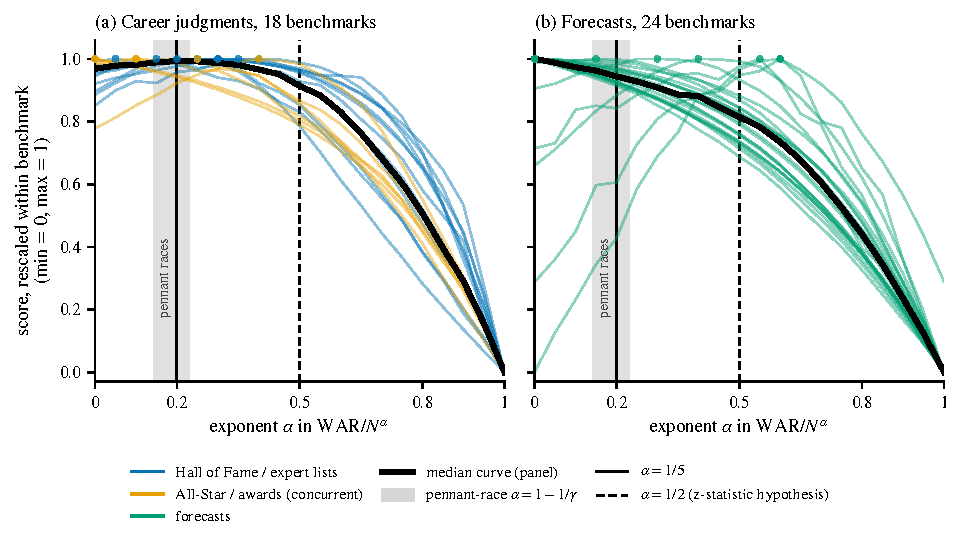
\includegraphics[width=\textwidth]{figures/fig_alpha_curves.pdf}
\caption{Every benchmark as a function of the exponent $\alpha$ in $Z_\alpha = \WAR/N^{\alpha}$, rescaled within each benchmark (minimum over $\alpha$ $= 0$, maximum $= 1$). Dots mark each curve's maximum; thick lines are the median rescaled curve in each panel. (a)~Judgments of finished careers (Hall of Fame in eight pools and two expert top-100 lists, blue) and concurrent season honors (career All-Star selections and award shares, orange). (b)~Forecasts of future $\WAR$, All-Star selections, award shares and Hall of Fame election from early-career checkpoints and first-half careers. The shaded band is the pennant-race estimate $\alpha = 1 - 1/\gamma$ of Section~\ref{sec:gamma}; the solid line marks $\alpha = \tfrac15$ and the dashed line the $z$-statistic hypothesis $\alpha = \tfrac12$.}
\label{fig:curves}
\end{figure}

\begin{table}[htbp]
\centering
\caption{Summary of the $42$ benchmarks by group. $\hat\alpha$: exponent maximizing each benchmark's metric on a $0.05$ grid (median and interquartile range across benchmarks). ``Interval contains'': number of benchmarks whose 95\% bootstrap interval for $\hat\alpha$ contains $\tfrac15$ / $\tfrac12$. ``$\tfrac15$ vs.\ $\tfrac12$'' and ``$\tfrac15$ vs.\ $0$'': number of benchmarks on which $\alpha = \tfrac15$ scores higher, with the number of 95\% bootstrap intervals for the difference that exclude zero in favor of $\tfrac15$ / against it in parentheses. Regret is the shortfall of a fixed exponent from each benchmark's best exponent, in AUC or Spearman units (mean / maximum over the group). The pennant-race estimates (Table~\ref{tab:gamma}) give $\alpha = 0.14$--$0.23$. Regret-minimizing exponents (minimax / min-mean): judgments 0.20 / 0.20; concurrent honors 0.20 / 0.10; forecasts, hitters 0.10 / 0.00; forecasts, pitchers 0.00 / 0.00; all benchmarks 0.15 / 0.15.}
\label{tab:convergence}
\footnotesize
\resizebox{\textwidth}{!}{%
\begin{tabular}{@{}lrcccccccc@{}}
\toprule
 & & & \multicolumn{2}{c}{\textbf{Interval contains}} & & & \multicolumn{3}{c}{\textbf{Regret (mean / max)}} \\
\cmidrule(lr){4-5} \cmidrule(lr){8-10}
\textbf{Group} & $n$ & $\hat\alpha$ median (IQR) & $\tfrac15$ & $\tfrac12$ & $\tfrac15$ vs.\ $\tfrac12$ & $\tfrac15$ vs.\ $0$ & $\alpha = 0$ & $\alpha = \tfrac15$ & $\alpha = \tfrac12$ \\
\midrule
Judgments of finished careers & 12 & 0.25 (0.24--0.30) & 12 & 5 & 10 (1 / 0) & 11 (3 / 0) & 0.0081 / 0.0167 & 0.0012 / 0.0035 & 0.0121 / 0.0314 \\
Concurrent season honors & 6 & 0.10 (0.03--0.21) & 4 & 2 & 5 (2 / 0) & 3 (1 / 2) & 0.0065 / 0.0327 & 0.0058 / 0.0114 & 0.0242 / 0.0385 \\
Forecasts, hitters & 12 & 0.07 (0.00--0.44) & 7 & 6 & 8 (5 / 0) & 6 (1 / 4) & 0.0015 / 0.0055 & 0.0025 / 0.0080 & 0.0072 / 0.0265 \\
Forecasts, pitchers & 12 & 0.00 (0.00--0.00) & 5 & 0 & 12 (12 / 0) & 0 (0 / 6) & 0.0000 / 0.0000 & 0.0047 / 0.0179 & 0.0197 / 0.0639 \\
\midrule
All benchmarks & 42 & 0.08 (0.00--0.29) & 28 & 13 & 35 (20 / 0) & 20 (5 / 12) & 0.0037 / 0.0327 & 0.0032 / 0.0179 & 0.0146 / 0.0639 \\
\bottomrule
\end{tabular}%
}
\end{table}


Four patterns stand out.
\begin{enumerate}
    \item \emph{$H_{1/2}$ fails.} Across the $42$ benchmarks, $\alpha = \tfrac15$ scores at least as well as $\alpha = \tfrac12$ in $35$, and the bootstrap interval for the difference excludes zero in favor of $\tfrac15$ in $20$ and in favor of $\tfrac12$ in none. Only $13$ of the $42$ argmax intervals contain $\tfrac12$. Even where a curve peaks near $\tfrac12$ (hitter checkpoints, the pools with relievers), the advantage over $\tfrac15$ is a few thousandths and never significant. The regression-implied exponents, which do not depend on the grid, rank the benchmarks in nearly the same order as $\hat\alpha$ (Spearman correlation $0.79$; Appendix~\ref{app:benchmarks}).
    \item \emph{Judgments of career value peak near $\tfrac15$, next to where pennant races put it.} The twelve Hall of Fame and expert-list benchmarks have a median $\hat\alpha$ of $0.25$ (interquartile range $0.24$--$0.30$; six of the twelve lie in $[0.15, 0.25]$ and nine in $[0.15, 0.30]$), every one of their intervals contains $0.2$, and $\alpha = \tfrac15$ beats career $\WAR$ in eleven of the twelve. Their regression-implied exponents have median $0.26$, and each lies inside the corresponding argmax interval. Their regret, the criterion that pools them, is smallest at exactly $\alpha = 0.20$. The pennant-race estimate, made before any player benchmark was consulted, is $0.14$--$0.23$ (shaded band): adjacent to the judgments' optimum and overlapping their intervals, slightly below their median.
    \item \emph{Forecasts of cumulative outcomes prefer smaller exponents still.} The median forecast $\hat\alpha$ is $0$: career $\WAR$ is the best predictor of every pitcher outcome and of every outcome in the midpoint design, and across all $42$ benchmarks it beats $\alpha = \tfrac15$ significantly on $12$ (and loses significantly on $5$). Proposition~\ref{prop:target} suggests why: a forecast of a future total rewards current playing time to the extent that playing time persists, and it persists more than rate does (Section~\ref{sec:forecast}). Concurrent honors that are themselves totals (career All-Star selections and award shares for hitters) behave the same way. Targets that are rates mostly behave the opposite way: at checkpoints, future per-event rate is best predicted by $\alpha = 0.95$--$1$ (in the midpoint design, $0.70$ for hitters but $0.20$ for pitchers; Appendix~\ref{app:benchmarks}).
    \item \emph{No single exponent is optimal for every target, but $\alpha \approx \tfrac15$ is the best single choice.} If one exponent must serve every benchmark, the natural criterion is regret, the shortfall from each benchmark's own best exponent. Across all $42$ benchmarks, both the maximum and the mean regret are smallest at $\alpha = 0.15$ ($0.017$ and $0.0029$), with $\alpha = 0.2$ essentially tied ($0.018$ and $0.0032$), against $0.033$ and $0.0037$ for career $\WAR$ and $0.064$ and $0.0146$ for $\alpha = \tfrac12$. Mean regret is nearly flat between $0.10$ and $0.15$ ($0.0029$), and the minimax point is set by just two benchmarks (dropping either moves it to $0.10$ or $0.20$), so the data locate the best compromise at $0.10$--$0.20$ rather than at a sharp point. Within the judgment benchmarks both criteria select $\alpha = 0.20$ exactly.
\end{enumerate}

\subsection{Hall of Fame}
\label{sec:hof}

We use all players on Baseball-Reference's JAWS position pages whose final season was 2010 or earlier, so that BBWAA eligibility has run its course. The main specification excludes players whose outcomes were driven by bans or PED controversy (Rose, Joe Jackson, Bonds, Clemens, McGwire, Sosa, Palmeiro, Sheffield); including them changes AUCs by at most $0.003$. Hitters are scored with position-player $\WAR$ and $\PA$, pitchers with pitching $\WAR$ and $\BF$; published pitcher $\JAWS$ includes batting value while our pitcher scores do not, which matters little (scoring starters by the two-coordinate score raises their $Z_{1/2}$ AUC from $0.904$ to $0.910$). $\WAA$ is Baseball-Reference's published Wins Above Average. The Hall of Fame flag includes committee selections (including Negro Leagues electees) and players elected primarily in other roles. Table~\ref{tab:hof} reports the AUC for classifying Hall of Famers.

\begin{table}[htbp]
\centering
\caption{Hall of Fame classification AUC (final season $\le 2010$; banned/PED cases excluded). ``Contested'' restricts to career $\WAR \ge 40$ (position-player $\WAR$ for hitters, pitching $\WAR$ for SP). In the $\JAWS$ column, $\SJAWS$ (SP, Hitters + SP), $\RJAWS$ (RP) and the role-appropriate one of the two (SP + RP) are in parentheses. SPW is Gordon's Standardized Peak WAR \cite{gordon2023}. $\hat\alpha$ is the in-sample AUC-maximizing exponent on a $0.05$ grid with its 95\% bootstrap interval ($1{,}000$ stratified resamples); ``CV'' is the mean held-out AUC when $\alpha$ is chosen on training folds ($20\times$ repeated stratified 5-fold CV). The best of $Z_{1/5}$ and $Z_{1/2}$ in each row is in bold.}
\label{tab:hof}
\footnotesize
\resizebox{\textwidth}{!}{%
\begin{tabular}{@{}lrrcccccccccc@{}}
\toprule
\textbf{Pool} & $n$ & HOF & $\WAR$ & $\WAR_7$ & $\JAWS$ & $\WAA$ & SPW & $Z_{1/5}$ & $Z_{1/2}$ & $\hat\alpha$ (AUC) & 95\% interval & CV \\
\midrule
Hitters (8 positions pooled) & 3,012 & 199 & 0.935 & 0.932 & 0.936 & 0.925 & 0.931 & \textbf{0.936} & 0.935 & 0.25 (0.936) & [0.00, 0.55] & 0.935 \\
Starting pitchers & 410 & 74 & 0.910 & 0.883 & 0.909 (0.910) & 0.890 & 0.877 & \textbf{0.914} & 0.904 & 0.25 (0.914) & [0.00, 0.45] & 0.909 \\
Relief pitchers & 280 & 8 & 0.976 & 0.948 & 0.974 (0.992) & 0.975 & 0.984 & 0.984 & \textbf{0.985} & 0.35 (0.988) & [0.05, 0.60] & 0.984 \\
Hitters + SP pooled & 3,422 & 273 & 0.936 & 0.927 & 0.935 (0.936) & 0.928 & 0.929 & \textbf{0.938} & 0.935 & 0.25 (0.938) & [0.10, 0.40] & 0.938 \\
SP + RP pooled & 690 & 82 & 0.929 & 0.900 & 0.921 (0.920) & 0.923 & 0.925 & 0.938 & \textbf{0.939} & 0.40 (0.941) & [0.20, 0.55] & 0.938 \\
\midrule
Contested hitters & 281 & 154 & 0.825 & 0.795 & 0.828 & 0.808 & 0.790 & \textbf{0.836} & 0.821 & 0.20 (0.836) & [0.05, 0.35] & 0.831 \\
Contested SP & 149 & 65 & 0.832 & 0.767 & 0.822 (0.827) & 0.788 & 0.755 & \textbf{0.830} & 0.808 & 0.05 (0.833) & [0.00, 0.40] & 0.821 \\
Contested hitters + SP & 430 & 219 & 0.822 & 0.756 & 0.808 (0.821) & 0.798 & 0.777 & \textbf{0.838} & 0.807 & 0.25 (0.839) & [0.05, 0.35] & 0.836 \\
\bottomrule
\end{tabular}%
}
\end{table}


\begin{itemize}
    \item \emph{$Z_{1/5}$ matches or beats the standard benchmarks.} At $\alpha = \tfrac15$ the family matches or exceeds career $\WAR$ and $\JAWS$ in seven of eight pools; the exception is contested starters ($0.830$ vs.\ $0.832$ for $\WAR$). The differences are small for hitters (intervals $[-0.001, +0.003]$ against $\WAR$ and $[-0.003, +0.004]$ against $\JAWS$) but significant in the two pools that contain relievers (starters plus relievers: $[+0.001, +0.016]$ against $\WAR$ and $[+0.003, +0.031]$ against $\JAWS$; relievers: $[+0.000, +0.020]$ and $[+0.001, +0.023]$) and against $\JAWS$ in the contested hitter-plus-starter sample ($[+0.004, +0.056]$). (The reliever interval touches zero in the $1{,}000$-resample bootstrap summarized in Table~\ref{tab:convergence}, so that comparison is borderline.) Under cross-validation, fixed $\alpha = \tfrac15$ does at least as well as the exponent chosen on training folds in all eight pools (Appendix~\ref{app:hof}). The purpose-built $\RJAWS$ remains best for relievers alone.
    \item \emph{$Z_{1/2}$ is no better than career $\WAR$.} For pooled hitters the intervals for the AUC difference between $\ZWAR$ and another metric are $[-0.008, +0.007]$ against $\JAWS$ and $[-0.006, +0.006]$ against $\WAR$, and against $Z_{1/5}$ $\ZWAR$ loses in six of eight pools, significantly in the contested hitter-plus-starter sample ($0.807$ vs.\ $0.838$; $[+0.010, +0.051]$). The AUC is nearly flat for $\alpha \in [0, 0.4]$ and falls steadily beyond ($0.930$ at $0.7$, $0.896$ at $1$ for pooled hitters), so the Hall of Fame identifies the exponent only weakly; but it places the plateau below $\tfrac12$ in every pool without relievers.
    \item \emph{Relievers are where $\tfrac12$ comes closest.} In the pooled starter-plus-reliever sample, $\ZWAR$ has the highest AUC ($0.939$), with $Z_{1/5}$ close behind ($0.938$; difference $[-0.014, +0.010]$), against $0.929$ for $\WAR$ and $0.921$ for $\JAWS$. Here the argmax is $0.40$ $[0.20, 0.55]$, the one judgment benchmark whose interval only just contains $\tfrac15$. Hall of Fame voting has rewarded relievers, largely through saves, more than their season value (Section~\ref{sec:value}), and a larger exponent reproduces that premium. Under $\WAR$, the eight relief Hall of Famers rank $47$th to $356$th in the combined pitcher list; under $Z_{1/5}$, $45$th to $316$th; under $\ZWAR$, $41$st to $297$th.
    \item \emph{Volume is rewarded, but not linearly.} By Proposition~\ref{prop:alpha}, $\alpha = \tfrac12$ penalizes any additional season below half a player's career rate (an All-Star pace for an inner-circle hitter), whereas $\alpha \approx \tfrac15$--$\tfrac14$ sets the dilution threshold at one-fifth to one-quarter of the career rate (roughly a league-average regular), rewarding solid late-career seasons and discounting only near-replacement play. By Proposition~\ref{prop:gamma}, voters behave as if season value were mildly convex, $\gamma \approx 1.25$--$1.33$, as pennant races are.
    \item \emph{$\PA \equiv \BF$ is not contradicted} (tested at $\alpha = \tfrac12$). In the pooled hitter and starter sample, multiplying pitcher scores by $c \in \{0.8, 0.9, \ldots, 1.4\}$ at $\alpha = \tfrac12$ gives AUCs of $0.926$--$0.937$; the unscaled $c = 1$ is within $0.002$ of the best value, and the variance-based $c \approx 0.98$--$1.01$ (Section~\ref{sec:zstat}) gives $0.934$--$0.935$.
    \item \emph{Caveats.} In pools that mix hitters and pitchers, changing $\alpha$ also changes the relative scale of the groups, because starters accumulate roughly twice as many events; the best $\alpha$ there mixes the effect of the exponent with that of a cross-role factor. We report many pools, metrics and intervals without a multiplicity adjustment.
\end{itemize}

\subsection{Expert rankings}
\label{sec:expert}

The Sporting News's 1998 list \cite{tsn1998} and ESPN's 2022 list, compiled from more than $20{,}000$ votes by ESPN writers and editors \cite{espn2022}, both include Negro Leagues stars, pitchers ($28$ and $27$ of the $100$, counting a player as a pitcher if his pitching $\WAR$ exceeds his batting $\WAR$) and then-active players. Each player is therefore scored on his record through the last season completed before publication (1997 and 2021). The universe is every player in Baseball-Reference's MLB and Negro Leagues season files with at least $15$ career $\WAR$ through that season ($1{,}592$ and $2{,}082$ players; every listed player qualifies). Two-way records are combined with Definition~\ref{def:twoway}, and $\JAWS$ is recomputed from seasons through the same cutoff. Table~\ref{tab:expert} reports the results.

\begin{table}[htbp]
\centering
\caption{Agreement with expert top-100 lists, careers through the season before publication. Entries are the Spearman correlation with list order among the $100$ listed players / the AUC for list membership in the universe; the second row of each list gives the number of pitchers in the metric's top $100$ (lists: $28$ and $27$). Two-way records are combined by Definition~\ref{def:twoway}; $c$ multiplies pitcher scores. The final column gives the in-sample optimal exponents $\hat\alpha_\rho$ / $\hat\alpha_{\mathrm{AUC}}$ on a $0.05$ grid (achieving $\rho = 0.578$, $\mathrm{AUC} = 0.960$ on Sporting News 1998 and $\rho = 0.575$, $\mathrm{AUC} = 0.981$ on ESPN 2022).}
\label{tab:expert}
\footnotesize
\setlength{\tabcolsep}{4pt}
\resizebox{\textwidth}{!}{%
\begin{tabular}{@{}llccccccccc@{}}
\toprule
 & & & & & & & & $Z_{1/2}$ & $Z_{1/2}$ & $\hat\alpha$ \\
\textbf{List} & & $\WAR$ & $\JAWS$ & $Z_{1/5}$ & $Z_{1/4}$ & $Z_{1/2}$ & $Z_1$ & ($c = 1.2$) & ($c = 59/41$) & ($\rho$ / AUC) \\
\midrule
Sporting News 1998 & $\rho$ / AUC & 0.565 / 0.954 & 0.592 / 0.951 & 0.577 / 0.960 & 0.577 / 0.960 & 0.558 / 0.954 & 0.310 / 0.816 & 0.623 / 0.960 & 0.646 / 0.954 & 0.30 / 0.30 \\
($n = 1{,}592$) & pitchers & 33 & 39 & 22 & 20 & 10 & 13 & 24 & 47 & \\
\midrule
ESPN 2022 & $\rho$ / AUC & 0.560 / 0.976 & 0.586 / 0.974 & 0.573 / 0.980 & 0.567 / 0.981 & 0.551 / 0.976 & 0.311 / 0.828 & 0.613 / 0.980 & 0.621 / 0.973 & 0.15 / 0.30 \\
($n = 2{,}082$) & pitchers & 33 & 38 & 28 & 25 & 13 & 14 & 29 & 51 & \\
\bottomrule
\end{tabular}%
}
\end{table}


\begin{itemize}
    \item \emph{Experts, like voters, favor $\alpha \approx \tfrac15$.} Both lists' curves are nearly flat for $\alpha \in [0, 0.4]$, peak at $\alpha = 0.15$--$0.30$, and fall steadily beyond $\alpha = 0.5$; a pure rate does poorly. The membership argmax intervals ($[0.15, 0.40]$ for both lists) exclude both $0$ and $\tfrac12$, and $Z_{1/4}$ beats career $\WAR$ in membership AUC (intervals $[+0.001, +0.012]$ and $[+0.000, +0.009]$). List order, among only $100$ players, identifies the exponent poorly ($[0, 0.65]$ and $[0, 0.55]$). $\ZWAR$ is statistically indistinguishable from career $\WAR$ and from $\JAWS$.
    \item \emph{The exponent sets the pitcher share.} With no scale factor, $\ZWAR$ places only $10$ and $13$ pitchers in its top $100$, against $27$--$28$ on the lists. $Z_{1/5}$ places $22$ and $28$ (and $28$ on the 2026 all-time list; Section~\ref{sec:unified_empirical}), close to the lists. To match the lists at $\alpha = \tfrac12$ one needs a pitcher scale factor of about $c = 1.2$, which also raises the Spearman correlation with list order from $0.558$ and $0.551$ to $0.623$ and $0.613$; but $c = 1.2$ was chosen to match the lists, and at $\alpha = \tfrac15$ no factor is needed.
\end{itemize}

\subsection{Forecasts and the scaling of targets}
\label{sec:forecast}

\paragraph{Design.} For every player whose career began in 1901 or later and includes no Negro Leagues season (whose records are incomplete), we take as the checkpoint the end of his third or fifth season in a role, requiring at least $1{,}000\,\PA$ (hitters, defined as players with fewer than $100$ career innings pitched) or $600\,\BF$ (pitchers, scored on pitching $\WAR$ alone; $\BF$ is approximated as $1.4\times$ outs recorded). In the midpoint design we take careers of at least six seasons in the role and split them after $\lfloor S/2 \rfloor$ seasons, with the same exposure minimum in the first half. Outcomes are measured after the split: future $\WAR$ (careers ending by 2023 for checkpoints, by 2016 otherwise), future All-Star selections (from 1933), future award shares (MVP from 1931 for hitters; MVP plus Cy Young from 1956 for pitchers), all as Spearman correlations, and Hall of Fame election as an AUC (careers ending by 2010, with the exclusions above). All-Star and award data come from the Baseball Databank \cite{lahman}, mapped to Baseball-Reference identifiers (award voting ends in 2016 and All-Star rosters in 2019; we apply a common 2016 career cutoff). As a contrast we also predict the future per-event rate. Table~\ref{tab:forecast} reports the results.

\begin{table}[htbp]
\centering
\caption{Forecasts from early-career checkpoints (after three or five seasons in the role) and from the first half of a career (midpoint split). Entries are the exponent $\hat\alpha$ that maximizes the Spearman correlation with the future outcome (AUC for Hall of Fame election), with its 95\% bootstrap interval; $^{\dagger}$ marks intervals that exclude $\tfrac15$. Last three columns: exposure persistence $\beta$ (slope of $\log N_{\mathrm{future}}$ on $\log N$), rate persistence $\kappa$ (slope of $\log r_{\mathrm{future}}$ on $\log r$, players with positive $\WAR$ in both periods) and the Spearman correlation $\rho_r$ between early and future rates. If future rate and exposure were independent, Proposition~\ref{prop:target} would put the optimum for a cumulative target at $\alpha = 0$ whenever $\beta \ge \kappa$; this matches the pitcher and midpoint designs but not the hitter checkpoints (Section~\ref{sec:forecast}). Future $\WAR$ at checkpoints uses careers ending by 2023; all other outcomes careers ending by 2016 (Hall of Fame: by 2010).}
\label{tab:forecast}
\footnotesize
\resizebox{\textwidth}{!}{%
\begin{tabular}{@{}lccccccc@{}}
\toprule
 & \multicolumn{4}{c}{\textbf{$\hat\alpha$ [95\% interval] for the future outcome}} & \multicolumn{3}{c}{\textbf{Persistence}} \\
\cmidrule(lr){2-5} \cmidrule(l){6-8}
\textbf{Design} & $\WAR$ & All-Star selections & Award shares & Hall of Fame & $\beta$ & $\kappa$ & $\rho_r$ \\
\midrule
Hitters, 3 seasons & 0.60 [0.15, 0.95] & 0.00 [0.00, 0.75] & 0.60 [0.00, 0.95] & 0.55 [0.00, 0.95] & 1.26 & 0.42 & 0.53 \\
Hitters, 5 seasons & 0.40 [0.30, 0.55]$^{\dagger}$ & 0.00 [0.00, 0.35] & 0.15 [0.00, 0.45] & 0.30 [0.00, 0.50] & 1.63 & 0.49 & 0.58 \\
Hitters, Midpoint & 0.00 [0.00, 0.05]$^{\dagger}$ & 0.00 [0.00, 0.00]$^{\dagger}$ & 0.00 [0.00, 0.00]$^{\dagger}$ & 0.00 [0.00, 0.05]$^{\dagger}$ & 0.93 & 0.49 & 0.59 \\
\midrule
Pitchers, 3 seasons & 0.00 [0.00, 0.00]$^{\dagger}$ & 0.00 [0.00, 0.20] & 0.00 [0.00, 0.20] & 0.00 [0.00, 0.25] & 1.07 & 0.07 & 0.23 \\
Pitchers, 5 seasons & 0.00 [0.00, 0.00]$^{\dagger}$ & 0.00 [0.00, 0.10]$^{\dagger}$ & 0.00 [0.00, 0.05]$^{\dagger}$ & 0.00 [0.00, 0.30] & 1.40 & 0.03 & 0.24 \\
Pitchers, Midpoint & 0.00 [0.00, 0.00]$^{\dagger}$ & 0.00 [0.00, 0.05]$^{\dagger}$ & 0.00 [0.00, 0.00]$^{\dagger}$ & 0.00 [0.00, 0.20] & 0.87 & 0.19 & 0.26 \\
\bottomrule
\end{tabular}%
}
\end{table}


\begin{itemize}
    \item \emph{Pitchers: playing time is the best predictor.} Career $\WAR$ ($\alpha = 0$) is the best checkpoint and midpoint predictor of every pitcher outcome, and $\alpha = \tfrac15$ trails it only slightly (by $0.002$--$0.006$ at checkpoints) while beating $\alpha = \tfrac12$ significantly in every pitcher forecast. An early pitching workload carries information about role (starter or reliever) and durability that any exposure discount partly removes.
    \item \emph{Hitter checkpoints are flat.} After three or five seasons, hitters' curves vary by about $0.01$ or less across $\alpha \in [0, \tfrac12]$. Future $\WAR$ peaks at $0.40$--$0.60$, future All-Star selections at $0$, award shares at $0.15$--$0.60$. These are the forecasts in which $H_{1/2}$ does best, but $\alpha = \tfrac12$ never beats $\tfrac15$ significantly (for future $\WAR$, $[-0.007, +0.001]$ and $[-0.005, +0.001]$).
    \item \emph{The midpoint split strongly favors volume.} When the first half of a career predicts the second, every outcome peaks at $\alpha = 0$ for both hitters and pitchers, and $\tfrac12$ is significantly worse than $\tfrac15$ in all eight midpoint benchmarks.
    \item \emph{Target scaling explains the pattern.} Playing time persists strongly from the early to the later part of a career: the elasticity $\beta$ of future exposure with respect to early exposure is $0.87$--$1.63$ across designs (Table~\ref{tab:forecast}). Rate persists much less, especially for pitchers: the elasticity $\kappa$ of future rate with respect to early rate is $0.42$--$0.49$ for hitters and $0.03$--$0.19$ for pitchers, and the rank correlation of early with future rates is $0.53$--$0.59$ and $0.23$--$0.26$. With $\beta \gg \kappa$, the independence version of Proposition~\ref{prop:target} puts the optimum for a cumulative target at or below $\alpha = 0$, which is what every pitcher design and both midpoint designs show; regressing each of these targets on $\log W$ and $\log N$ gives negative implied exponents. The simple formula $1 - \beta/\kappa$ is a guide to sign and ordering, not a quantitative fit: it ignores that future playing time itself responds to early rate (hitters who start well play more), and for hitter checkpoints, where rates persist most, it is far below the interior optimum of $0.4$--$0.6$. A two-equation version that lets exposure and rate each depend on both early quantities moves in the right direction but does not close the gap: $0.37$ $[-0.35, 0.99]$ after three seasons (consistent with the observed $0.60$) and $-0.21$ $[-0.83, 0.24]$ after five (below the observed interval $[0.30, 0.55]$). Why hitters' checkpoint forecasts favor interior exponents is therefore only partly explained.
    \item \emph{Rates are a different target.} At checkpoints, future per-event rate is best predicted by exponents near $1$ (hitters $0.95$, pitchers $1.0$), and the empirical Bayes rate matches or beats every member of the family, as Remark~\ref{rem:talent} anticipates. (In the midpoint design the optimum is $0.70$ for hitters and $0.20$ for pitchers, whose rates persist least.) Neither $Z_{1/5}$ nor $Z_{1/2}$ is a talent estimator.
\end{itemize}
These samples condition on reaching the checkpoint, and future playing time partly reflects decisions made on early performance, so the correlations describe forecasting value, not causal effects.

\subsection{Where \texorpdfstring{$\alpha = \tfrac12$}{alpha = 1/2} holds up}
\label{sec:half}

The hypothesis $H_{1/2}$ is not without support. $\alpha = \tfrac12$ scores above $\tfrac15$ on seven benchmarks, all by small and non-significant margins: hitters' future $\WAR$ after three and after five seasons (where the optima are $0.60$ and $0.40$), hitters' Hall of Fame election and MVP shares after three seasons, Hall of Fame classification in the two pools with relievers, where it reproduces the premium voters have given closers, and relievers' career All-Star selections. Appendix~\ref{app:null} shows that testing against nulls that are actually in doubt (league average, an All-Star pace) does not rescue it as a summary of career value: at $\alpha = \tfrac12$, Hall of Fame AUC falls monotonically as the null rises, in every pool. What the evidence reading does supply is the family's unit: one plate appearance carries the same information as one batter faced, and events classify Hall of Famers better than season counts in every pool (Appendix~\ref{app:seasons}).

\section{All-Time Leaderboards at \texorpdfstring{$\alpha = \tfrac15$}{alpha = 1/5}}
\label{sec:empirical}

All values use Baseball-Reference $\WAR$ ($\mathrm{bWAR}$) \cite{bbref2026}, accessed 16 October 2026. Ranks are among all players in Baseball-Reference's MLB and Negro Leagues season files. Career $\BF$ comes from the JAWS pages or player pages where available; for the remaining pitchers it is estimated as $4.2\,\BF$ per inning, which affects no pitcher ranked in the top $370$ at $\alpha = \tfrac15$. Every table is sorted by $Z_{1/5}$ and also shows the career-$\WAR$ rank ($\alpha = 0$) and the $Z_{1/2}$ rank, so that the reader can see what the exponent does at both ends. A $\pm 0.05$ change in published $\WAR$ moves $Z_{1/5}$ by $0.05/N^{0.2}$, about $0.006$--$0.010$ for the players shown; we treat gaps in $Z_{1/5}$ below $0.10$ (about $0.5\%$ of a top score, the same relative tolerance as $0.005$ on the $Z_{1/2}$ scale) as ties. Below the top fifty the boards are dense, and ranks there are resolved only to within a few places (Appendix~\ref{app:uncert}).

\subsection{Position play}
\label{sec:hitters}

\begin{table}[htbp]
\centering
\caption{Position-play coordinate at $\alpha = \tfrac15$, $Z_{1/5} = \WAR_{\mathrm{pos}} / \max(\PA, 1)^{1/5}$ (position-player $\mathrm{bWAR}$) \cite{bbref2026}, sorted by $Z_{1/5}$. All ranks are all-time position-play ranks: $\WAR$ \textbf{Rk} is the career-$\WAR$ rank ($\alpha = 0$; tied totals share the better rank) and $Z_{1/2}$ \textbf{Rk} the rank under $\Zpos = \WAR_{\mathrm{pos}}/\sqrt{\PA}$. $\JAWS$ ranks are across all eight fielding positions combined. The full two-coordinate valuation appears in Tables~\ref{tab:twoway}--\ref{tab:unified}.}
\label{tab:hitters}
\footnotesize
\setlength{\tabcolsep}{5pt}
\resizebox{\textwidth}{!}{%
\begin{tabular}{@{}clccccccc@{}}
\toprule
$Z_{1/5}$ \textbf{Rk} & \textbf{Player} & \textbf{Pos $\WAR$} & \textbf{Career $\PA$} & $\WAR / 650\text{ }\PA$ & $\JAWS$ \textbf{(Rk)} & $\WAR$ \textbf{Rk} & $Z_{1/2}$ \textbf{Rk} & $Z_{1/5} = \dfrac{\WAR_{\mathrm{pos}}}{\PA^{1/5}}$ \\
\midrule
\textbf{1} & Babe Ruth & 162.3 & 10,628 & \textbf{9.93} & 123.5 (\#1) & 2 & 1 & \textbf{25.41} \\
\textbf{2} & Barry Bonds & 162.8 & 12,606 & 8.39 & 117.8 (\#2) & 1 & 2 & \textbf{24.63} \\
\textbf{3} & Willie Mays & 156.2 & 12,545 & 8.09 & 114.9 (\#3) & 3 & 3 & \textbf{23.66} \\
\textbf{4} & Ty Cobb & 149.8 & 13,103 & 7.43 & 108.9 (\#4) & 4 & 4 & \textbf{22.49} \\
\textbf{5} & Hank Aaron & 143.2 & 13,941 & 6.68 & 101.8 (\#5) & 5 & 9 & \textbf{21.24} \\
\textbf{6} & Tris Speaker & 136.1 & 12,021 & 7.36 & 99.7 (\#7) & 6 & 6 & \textbf{20.79} \\
\textbf{7} & Rogers Hornsby & 127.4 & 9,481 & 8.73 & 100.7 (\#6) & 9 & 5 & \textbf{20.41} \\
\textbf{8} & Honus Wagner & 132.8 & 11,777 & 7.33 & 99.3 (\#8) & 7 & 8 & \textbf{20.37} \\
\textbf{9} & Stan Musial & 128.5 & 12,721 & 6.57 & 96.6 (\#9) & 8 & 11 & \textbf{19.41} \\
\textbf{10} & Ted Williams & 121.7 & 9,792 & 8.08 & 94.8 (\#10) & 11 & 7 & \textbf{19.37} \\
\textbf{11} & Eddie Collins & 123.7 & 12,087 & 6.65 & 93.7 (\#11) & 10 & 12 & \textbf{18.88} \\
\textbf{12} & Lou Gehrig & 113.5 & 9,665 & 7.63 & 90.6 (\#13) & 13 & 10 & \textbf{18.11} \\
\textbf{13} & Alex Rodriguez & 117.4 & 12,207 & 6.25 & 90.8 (\#12) & 12 & 15 & \textbf{17.88} \\
\textbf{14} & Mickey Mantle & 110.3 & 9,910 & 7.23 & 87.5 (\#14) & 16 & 13 & \textbf{17.51} \\
\textbf{15} & Mel Ott & 110.7 & 11,347 & 6.34 & 82.2 (\#18) & 15 & 17 & \textbf{17.11} \\
\midrule
\textbf{21} & Mike Trout & 91.7 & 7,837 & 7.61 & 78.3 (\#22) & 30 & 18 & \textbf{15.26} \\
\textbf{39} & Joe DiMaggio & 78.9 & 7,672 & 6.68 & 65.4 (\#39) & 43 & 27 & \textbf{13.19} \\
\textbf{61} & Pete Rose & 79.6 & 15,890 & 3.26 & 62.3 (\#45) & 41 & 143 & \textbf{11.50} \\
\textbf{70} & Jackie Robinson & 64.1 & 5,955 & 7.00 & 57.8 (\#65) & 106 & 40 & \textbf{11.27} \\
\textbf{109} & Turkey Stearnes & 55.2 & 4,378 & 8.20 & 45.1 (\#182) & 166 & 39 & \textbf{10.32} \\
\textbf{197} & Josh Gibson & 41.1 & 2,683 & \textbf{9.96} & 35.2 (\#371) & 345 & 50 & \textbf{8.47} \\
\bottomrule
\end{tabular}%
}
\end{table}


\begin{enumerate}
    \item \textbf{The top of the list is stable.} The $Z_{1/5}$ top fifteen are the career-$\WAR$ top sixteen without Rickey Henderson (\#18), reordered by at most two places, and Ruth leads Bonds clearly ($25.41$ vs.\ $24.63$). Ruth used $1{,}978$ fewer plate appearances for nearly the same position-player $\WAR$; Bonds leads in career $\WAR$ ($162.8$ vs.\ $162.3$), Ruth under every exponent above $0.02$.
    \item \textbf{What $\tfrac15$ changes relative to $\tfrac12$.} Long careers at high rates rise: Aaron (\#9 under $Z_{1/2}$ to \#5), Musial (\#11 to \#9), Alex Rodriguez and Mel Ott enter the top fifteen. Careers shortened by war service or illness keep only part of the lift $Z_{1/2}$ gave them: Ted Williams is \#10 (\#11 in $\WAR$, \#7 under $Z_{1/2}$), Gehrig \#12, DiMaggio \#39 (\#43, \#27). Crediting Williams with $2{,}000$ hypothetical extra $\PA$ at his career rate would raise his $\WAR$ by $20\%$, his $Z_{1/5}$ by $16\%$ and his $Z_{1/2}$ by $10\%$.
    \item \textbf{Peak versus volume.} Rose ($79.6\,\WAR$ in $15{,}890\,\PA$) and DiMaggio ($78.9$ in $7{,}672$) have nearly equal $\WAR$. $Z_{1/2}$ separates them by $116$ places (\#27 and \#143); at $\alpha = \tfrac15$ DiMaggio is still clearly ahead ($13.19$ vs.\ $11.50$), but by $22$ places (\#39 and \#61), because a threshold of one-fifth of the career rate counts most of Rose's long run of solid seasons in his favor.
    \item \textbf{Negro Leagues and color-barrier careers.} Turkey Stearnes (\#109), Jackie Robinson (MLB debut at 28; \#70) and Josh Gibson ($41.1\,\WAR$ in $2{,}683\,\PA$; \#197) all rank well above their career-$\WAR$ places (\#166, \#106, \#345) but far below their $Z_{1/2}$ places (\#39, \#40, \#50). Baseball-Reference's Negro Leagues statistics cover only documented games; event-based scores handle short \emph{schedules} better than season-window metrics, but they cannot correct for \emph{missing} records, so these placements carry extra uncertainty and depend strongly on the exponent.
\end{enumerate}

\subsection{Starting pitchers}
\label{sec:pitchers}

\begin{table}[htbp]
\centering
\caption{Starting pitchers ($\ge 1{,}500\,\IP$) at $\alpha = \tfrac15$, $Z_{1/5} = \WAR_{\mathrm{pitch}} / \max(\BF, 1)^{1/5}$ (pitching $\mathrm{bWAR}$) \cite{bbref2026}, sorted by $Z_{1/5}$. Columns 1 and 10 give the rank among these starters with the rank among \emph{all} pitchers in parentheses; $\WAR$ \textbf{Rk} ($\alpha = 0$; tied totals share the better rank) is also among all pitchers, and $Z_{1/2}$ is $\Zpitch = \WAR_{\mathrm{pitch}}/\sqrt{\BF}$. Baseball-Reference $\JAWS$ and $\SJAWS$ include pitcher batting.}
\label{tab:pitchers}
\footnotesize
\setlength{\tabcolsep}{5pt}
\resizebox{\textwidth}{!}{%
\begin{tabular}{@{}clccccccccc@{}}
\toprule
$Z_{1/5}$ \textbf{SP Rk} & & \textbf{Pitch} & \textbf{Career} & \textbf{Career $\IP$} & $\WAR\,/$ & $\JAWS$ & $\SJAWS$ & $\WAR$ & $Z_{1/2}$ \textbf{SP Rk} & $Z_{1/5} = $ \\
\textbf{(All)} & \textbf{Pitcher} & $\WAR$ & \textbf{$\BF$} & \textbf{($\BF/\IP$)} & $820\text{ }\BF$ & \textbf{(Rk)} & \textbf{(Rk)} & \textbf{Rk} & \textbf{(All)} & $\WAR_{\mathrm{pitch}}/\BF^{1/5}$ \\
\midrule
\textbf{1} (\#1) & Cy Young & 165.9 & 29,565 & 7,356.0 (4.02) & 4.60 & 120.8 (\#2) & 107.2 (\#2) & 1 & 3 (\#3) & \textbf{21.17} \\
\textbf{2} (\#2) & Walter Johnson & 155.4 & 23,415 & 5,914.1 (3.96) & 5.44 & 130.2 (\#1) & 117.6 (\#1) & 2 & 1 (\#1) & \textbf{20.78} \\
\textbf{3} (\#3) & Roger Clemens & 138.7 & 20,240 & 4,916.2 (4.12) & 5.62 & 102.6 (\#3) & 101.6 (\#3) & 3 & 2 (\#2) & \textbf{19.09} \\
\textbf{4} (\#4) & Kid Nichols & 119.0 & 21,099 & 5,067.1 (4.16) & 4.62 & 96.7 (\#4) & 83.1 (\#6) & 4 & 5 (\#5) & \textbf{16.24} \\
\textbf{5} (\#5) & Lefty Grove & 113.2 & 16,622 & 3,940.2 (4.22) & 5.58 & 86.2 (\#7) & 83.2 (\#5) & 6 & 4 (\#4) & \textbf{16.21} \\
\textbf{6} (\#6) & Grover Alexander & 116.9 & 20,893 & 5,190.0 (4.03) & 4.59 & 95.1 (\#5) & 85.1 (\#4) & 5 & 6 (\#6) & \textbf{15.99} \\
\textbf{7} (\#7) & Randy Johnson & 103.5 & 17,067 & 4,135.1 (4.13) & 4.97 & 81.3 (\#10) & 80.8 (\#9) & 9 & 8 (\#8) & \textbf{14.74} \\
\textbf{8} (\#8) & Tom Seaver & 106.0 & 19,369 & 4,783.0 (4.05) & 4.49 & 84.6 (\#8) & 81.9 (\#7) & 7 & 9 (\#10) & \textbf{14.72} \\
\textbf{9} (\#9) & Greg Maddux & 104.8 & 20,421 & 5,008.1 (4.08) & 4.21 & 81.4 (\#9) & 81.1 (\#8) & 8 & 11 (\#12) & \textbf{14.40} \\
\textbf{10} (\#10) & Christy Mathewson & 100.6 & 18,929 & 4,788.2 (3.95) & 4.36 & 88.8 (\#6) & 80.3 (\#10) & 10 & 12 (\#13) & \textbf{14.03} \\
\textbf{11} (\#11) & Pedro Mart\'{i}nez & 86.1 & 11,394 & 2,827.1 (4.03) & \textbf{6.20} & 71.1 (\#22) & 71.1 (\#12) & 17 & 7 (\#7) & \textbf{13.29} \\
\textbf{12} (\#12) & Bert Blyleven & 96.1 & 20,491 & 4,970.0 (4.12) & 3.85 & 72.4 (\#17) & 69.7 (\#15) & 12 & 16 (\#17) & \textbf{13.20} \\
\textbf{13} (\#13) & Phil Niekro & 97.0 & 22,677 & 5,404.0 (4.20) & 3.51 & 75.1 (\#15) & 70.1 (\#14) & 11 & 21 (\#22) & \textbf{13.05} \\
\textbf{14} (\#14) & Gaylord Perry & 93.0 & 21,953 & 5,350.0 (4.10) & 3.47 & 71.2 (\#21) & 65.7 (\#19) & 13 & 23 (\#24) & \textbf{12.59} \\
\textbf{15} (\#15) & Warren Spahn & 92.6 & 21,547 & 5,243.2 (4.11) & 3.52 & 75.8 (\#13) & 72.6 (\#11) & 14 & 22 (\#23) & \textbf{12.59} \\
\midrule
\textbf{20} (\#20) & Clayton Kershaw & 78.1 & 11,279 & 2,855.1 (3.95) & 5.68 & 65.3 (\#28) & 65.3 (\#20) & 28 & 10 (\#11) & \textbf{12.08} \\
\textbf{28} (\#28) & Nolan Ryan & 83.6 & 22,575 & 5,386.0 (4.19) & 3.04 & 62.2 (\#34) & 59.7 (\#30) & 20 & 45 (\#46) & \textbf{11.26} \\
\textbf{81} (\#83) & Satchel Paige & 48.7 & 7,331 & 1,800.0 (4.07) & 5.45 & 38.2 (\#173) & 38.2 (\#160) & 112 & 38 (\#39) & \textbf{8.21} \\
\textbf{89} (\#92) & Bill Foster & 45.6 & 6,213 & 1,509.0 (4.12) & \textbf{6.02} & 41.4 (\#138) & 41.4 (\#122) & 132 & 33 (\#34) & \textbf{7.95} \\
\bottomrule
\end{tabular}%
}
\end{table}


\begin{enumerate}
    \item \textbf{The top three follow career $\WAR$.} Cy Young ($21.17$) leads Walter Johnson ($20.78$) and Roger Clemens ($19.09$). Under $Z_{1/2}$ Johnson and Clemens pass Young, whose $29{,}565$ batters faced are penalized more heavily; at $\alpha = \tfrac15$ the order of the top three is decided by career value, not by the exposure unit. ($\JAWS$ and $\SJAWS$ rank Johnson first and Young second.)
    \item \textbf{Durable starters enter the top fifteen.} Blyleven (\#12), Niekro (\#13), Perry and Spahn (tied at $12.59$) replace shorter, higher-rate careers. Pedro Mart\'{i}nez ($6.20\,\WAR/820\,\BF$) is \#11 (\#7 under $Z_{1/2}$), and Clayton Kershaw falls to \#20, in a tie block with Mussina, Verlander and Schilling. The Kershaw--Maddux--Mathewson near-tie under $Z_{1/2}$ dissolves (Maddux \#9, Mathewson \#10).
    \item \textbf{Volume and short-schedule pitchers.} Nolan Ryan is \#28 (\#20 in $\WAR$, \#46 under $Z_{1/2}$), and his $4.19\,\BF/\IP$, among the highest in the table, adds to his event count. Negro Leagues aces Satchel Paige and Bill Foster rank \#83 and \#92 among all pitchers (\#39 and \#34 under $Z_{1/2}$), with the caveat of Section~\ref{sec:hitters}.
\end{enumerate}

\subsection{Relief pitchers on the starter scale}
\label{sec:relievers}

Full-time closers face $240$--$300$ batters per season ($2{,}900$--$5{,}400$ over a career), modern starters $650$--$850$. A reliever with one-quarter of a starter's $\BF$ needs $4^{1-\alpha}$ times the per-batter rate to match his score: about three times at $\alpha = \tfrac15$ and twice at $\alpha = \tfrac12$. On the season-value reading a relief season is worth only its $\WAR$, however few batters it took (Section~\ref{sec:value}), so any discount relative to $\WAR$ is a consequence of counting events, and it grows with $\alpha$. Leverage enters through the numerator: Baseball-Reference scales relief $\WAA$ by $(1+\overline{\mathrm{gmLI}})/2$ \cite{bbrefwarpitch}.

\begin{table}[htbp]
\centering
\caption{Relief pitchers and Hall of Fame starter benchmarks (italics) at $\alpha = \tfrac15$, $Z_{1/5} = \WAR_{\mathrm{pitch}} / \max(\BF, 1)^{1/5}$, sorted by $Z_{1/5}$ across \emph{all} pitchers \cite{bbref2026}. $\mathrm{RP}$ classification, $\mathrm{RP}$ ranks (column 2) and $\RJAWS$ ranks follow Baseball-Reference's Relief Pitcher JAWS leaderboard \cite{bbrefjawsrp}; Hybrid roles have $\ge 100$ starts. Parenthetical ranks after pitching $\WAR$ are career-$\WAR$ ranks ($\alpha = 0$) among all pitchers; $Z_{1/2}$ \textbf{Rk} is the all-pitcher rank under $\Zpitch = \WAR_{\mathrm{pitch}}/\sqrt{\BF}$ (RP rank in parentheses). Baseball-Reference $\JAWS$ and $\RJAWS$ include pitcher batting.}
\label{tab:relievers}
\footnotesize
\setlength{\tabcolsep}{4pt}
\resizebox{\textwidth}{!}{%
\begin{tabular}{@{}cclcccccccc@{}}
\toprule
\textbf{All-Pitch} & \textbf{RP} & \textbf{Pitcher} & \textbf{Pitch $\WAR$} & \textbf{Career} & \textbf{Career $\IP$} & $\WAR\,/$ & & $\RJAWS$ & $Z_{1/2}$ \textbf{Rk} & $Z_{1/5} = $ \\
$Z_{1/5}$ \textbf{Rk} & \textbf{Rk} & \textbf{(Role / HOF SP Benchmark)} & \textbf{(Rk)} & \textbf{$\BF$} & \textbf{($\BF/\IP$)} & $820\text{ }\BF$ & $\JAWS$ & \textbf{(RP Rk)} & \textbf{(RP)} & $\WAR_{\mathrm{pitch}}/\BF^{1/5}$ \\
\midrule
\textbf{7} & --- & \emph{Randy Johnson (HOF SP)} & \emph{103.5 (\#9)} & \emph{17,067} & \emph{4,135.1 (4.13)} & \emph{4.97} & \emph{81.3} & --- & \emph{8} & \emph{14.74} \\
\textbf{8} & --- & \emph{Tom Seaver (HOF SP)} & \emph{106.0 (\#7)} & \emph{19,369} & \emph{4,783.0 (4.05)} & \emph{4.49} & \emph{84.6} & --- & \emph{10} & \emph{14.72} \\
\textbf{28} & --- & \emph{Nolan Ryan (HOF SP)} & \emph{83.6 (\#20)} & \emph{22,575} & \emph{5,386.0 (4.19)} & \emph{3.04} & \emph{62.2} & --- & \emph{46} & \emph{11.26} \\
\textbf{34} & \textbf{1} & \textbf{Mariano Rivera} (Pure RP) & 56.3 (\#80) & 5,103 & 1,283.2 (3.98) & 9.05 & 42.5 & 48.9 (\#1) & 9 (1) & \textbf{10.21} \\
\textbf{49} & --- & \emph{Bob Feller (HOF SP)} & \emph{65.2 (\#46)} & \emph{16,180} & \emph{3,827.0 (4.23)} & \emph{3.30} & \emph{57.5} & --- & \emph{69} & \emph{9.39} \\
\textbf{53} & \textbf{2} & \textbf{Dennis Eckersley} (SP/RP Hybrid) & 62.3 (\#54) & 13,534 & 3,285.2 (4.12) & 3.77 & 49.9 & 39.6 (\#2) & 52 (2) & \textbf{9.29} \\
\textbf{54} & --- & \emph{Don Sutton (300-Win HOF SP)} & \emph{68.3 (\#35)} & \emph{21,631} & \emph{5,282.1 (4.09)} & \emph{2.59} & \emph{50.3} & --- & \emph{99} & \emph{9.28} \\
\textbf{57} & --- & \emph{Juan Marichal (HOF SP)} & \emph{61.8 (\#56)} & \emph{14,236} & \emph{3,507.0 (4.06)} & \emph{3.56} & \emph{57.3} & --- & \emph{63} & \emph{9.13} \\
\textbf{67} & --- & \emph{Jim Bunning (HOF SP)} & \emph{60.4 (\#65)} & \emph{15,618} & \emph{3,760.1 (4.15)} & \emph{3.17} & \emph{54.2} & --- & \emph{88} & \emph{8.76} \\
\textbf{77} & --- & \emph{Sandy Koufax (HOF SP)} & \emph{53.1 (\#90)} & \emph{9,497} & \emph{2,324.1 (4.09)} & \emph{4.58} & \emph{47.5} & --- & \emph{50} & \emph{8.50} \\
\textbf{87} & --- & \emph{Whitey Ford (HOF SP)} & \emph{53.6 (\#86)} & \emph{13,036} & \emph{3,170.1 (4.11)} & \emph{3.37} & \emph{45.8} & --- & \emph{95} & \emph{8.06} \\
\textbf{90} & \textbf{3} & \textbf{Hoyt Wilhelm} (Multi-IP RP) & 49.7 (\#108) & 9,164 & 2,254.1 (4.07) & 4.45 & 36.7 & 34.4 (\#3) & 62 (3) & \textbf{8.02} \\
\midrule
\textbf{124} & --- & \emph{Early Wynn (300-Win HOF SP)} & \emph{51.5 (\#96)} & \emph{19,408} & \emph{4,564.0 (4.25)} & \emph{2.18} & \emph{49.8} & --- & \emph{226} & \emph{7.15} \\
\textbf{131} & \textbf{4} & \textbf{Rich Gossage} (Multi-IP RP) & 41.6 (\#169) & 7,507 & 1,809.1 (4.15) & 4.54 & 36.4 & 29.5 (\#4) & 90 (4) & \textbf{6.98} \\
\textbf{177} & --- & \emph{Jack Morris (HOF SP)} & \emph{43.6 (\#150)} & \emph{16,120} & \emph{3,824.0 (4.22)} & \emph{2.22} & \emph{38.0} & --- & \emph{264} & \emph{6.28} \\
\textbf{222} & \textbf{5} & \textbf{Tom Gordon} (SP/RP Hybrid) & 35.0 (\#223) & 9,058 & 2,108.0 (4.30) & 3.17 & 29.1 & 23.6 (\#10) & 228 (20) & \textbf{5.66} \\
\textbf{228} & \textbf{6} & \textbf{John Hiller} (Multi-IP RP) & 31.0 (\#278) & 5,206 & 1,242.0 (4.19) & 4.88 & 28.4 & 18.1 (\#25) & 128 (9) & \textbf{5.60} \\
\textbf{245} & \textbf{7} & \textbf{Billy Wagner} (Pure RP) & 27.8 (\#339) & 3,600 & 903.0 (3.99) & 6.33 & 23.7 & 24.9 (\#6) & 100 (5) & \textbf{5.40} \\
\textbf{248} & \textbf{8} & \textbf{Ellis Kinder} (SP/RP Hybrid) & 30.9 (\#282) & 6,302 & 1,479.2 (4.26) & 4.02 & 26.7 & 21.5 (\#13) & 192 (14) & \textbf{5.37} \\
\textbf{255} & \textbf{9} & \textbf{Bobby Shantz} (SP/RP Hybrid) & 32.1 (\#262) & 8,045 & 1,935.2 (4.16) & 3.27 & 29.7 & 18.4 (\#24) & 243 (22) & \textbf{5.31} \\
\textbf{257} & \textbf{10} & \textbf{Lee Smith} (Pure RP) & 29.3 (\#314) & 5,388 & 1,289.1 (4.18) & 4.46 & 24.8 & 21.0 (\#15) & 164 (12) & \textbf{5.26} \\
\textbf{258} & \textbf{11} & \textbf{Trevor Hoffman} (Pure RP) & 28.1 (\#334) & 4,388 & 1,089.1 (4.03) & 5.25 & 23.7 & 27.2 (\#5) & 132 (10) & \textbf{5.25} \\
\textbf{275} & \textbf{13} & \textbf{Aroldis Chapman} (Pure RP) & 26.1 (\#373) & 3,554 & 873.0 (4.07) & 6.02 & 21.9 & 23.3 (\#11) & 120 (6) & \textbf{5.09} \\
\textbf{276} & \textbf{14} & \textbf{Joe Nathan} (Pure RP) & 26.4 (\#370) & 3,771 & 923.1 (4.08) & 5.74 & 24.2 & 24.3 (\#8) & 125 (7) & \textbf{5.09} \\
\textbf{312} & \textbf{17} & \textbf{Kenley Jansen} (Pure RP) & 24.7 (\#412) & 3,860 & 972.1 (3.97) & 5.25 & 20.8 & 24.9 (\#6) & 169 (13) & \textbf{4.74} \\
\textbf{320} & \textbf{20} & \textbf{Jonathan Papelbon} (Pure RP) & 23.3 (\#457) & 2,938 & 725.2 (4.05) & 6.50 & 21.4 & 21.7 (\#12) & 127 (8) & \textbf{4.72} \\
\textbf{346} & \textbf{25} & \textbf{Bruce Sutter} (Pure RP) & 24.4 (\#428) & 4,251 & 1,042.0 (4.08) & 4.71 & 24.1 & 18.1 (\#25) & 222 (19) & \textbf{4.59} \\
\textbf{348} & \textbf{27} & \textbf{Tom Henke} (Pure RP) & 23.0 (\#465) & 3,194 & 789.2 (4.04) & 5.90 & 20.2 & 19.4 (\#19) & 146 (11) & \textbf{4.58} \\
\textbf{365} & \textbf{28} & \textbf{Craig Kimbrel} (Pure RP) & 22.7 (\#478) & 3,502 & 867.2 (4.04) & 5.32 & 21.0 & 19.7 (\#18) & 203 (15) & \textbf{4.44} \\
\bottomrule
\end{tabular}%
}
\end{table}


\begin{enumerate}
    \item \textbf{Rivera.} Mariano Rivera has $56.3\,\WAR$ in $5{,}103\,\BF$, and his $9.05\,\WAR/820\,\BF$ is the highest career rate of any pitcher with at least $2{,}000\,\BF$. He is \#34 among all pitchers at $\alpha = \tfrac15$ (\#80 in pitching $\WAR$, \#9 under $Z_{1/2}$), between Hall of Fame starters Ryan and Feller, and still first among relievers.
    \item \textbf{Durable relievers rise, one-inning closers fall.} Below Rivera, Eckersley (tied with Sutton) and Wilhelm, the reliever top ten at $\alpha = \tfrac15$ is mostly multi-inning relievers and swingmen: Gossage, Tom Gordon (\#20 among relievers under $Z_{1/2}$, \#5 here), Hiller, Kinder and Shantz. One-inning closers rank \#245--\#365 among all pitchers, behind 300-game winner Early Wynn (\#124) and Jack Morris (\#177); under $Z_{1/2}$ Billy Wagner (\#100) was level with Don Sutton (\#99). Whether Wagner belongs alongside Sutton or behind Morris is a question about the exponent, not about Wagner.
\end{enumerate}

\subsection{Two-way players}
\label{sec:twoway_empirical}

\begin{table}[htbp]
\centering
\caption{Two-coordinate valuation at $\alpha = \tfrac15$ for all $n = 18$ players with $\ge 10\,\WAR$ in both coordinates \cite{bbref2026}, sorted by the $\ell_\gamma$ combination $\Ztwoway = \sgn(\Ical_\gamma)|\Ical_\gamma|^{1/\gamma}$, $\Ical_\gamma = \sum_k \sgn(\WAR_k)|\WAR_k|^{\gamma}/N_k^{\gamma-1}$, with $\gamma = 1/(1-\alpha) = \tfrac54$ at $\alpha = \tfrac15$. $\Zpos$ and $\Zpitch$ are the single-coordinate $Z_{1/5}$ scores and $\Zpool = (\WAR_{\mathrm{pos}} + \WAR_{\mathrm{pitch}})/(\PA + \BF)^{1/5}$; percentage changes are relative to $\max(\Zpos, \Zpitch)$. Column 1 gives the rank among the 18 with the all-time unified rank in parentheses; $Z_{1/2}$ \textbf{Rk} is the rank among the 18 under Equation~\eqref{eq:universal_zwar} ($\gamma = 2$). Total $\WAR$ is the sum of the rounded components (Baseball-Reference lists Ruth's total as $182.6$ and Ruffing's as $68.6$); $^{*}$$\BF$ estimated at $4.2$ per inning (Elmer Smith, Cy Seymour).}
\label{tab:twoway}
\footnotesize
\setlength{\tabcolsep}{4pt}
\resizebox{\textwidth}{!}{%
\begin{tabular}{@{}clcccccccc@{}}
\toprule
& \textbf{Player} & \textbf{Pos $\WAR$} & \textbf{Pitch $\WAR$} & \textbf{Total} & & & $\Zpool$ & $Z_{1/2}$ & $\Ztwoway$ \\
\textbf{Rk (All)} & \textbf{(Role Profile)} & \textbf{($\PA$)} & \textbf{($\BF$ / $\IP$)} & \textbf{$\WAR$} & $\Zpos$ & $\Zpitch$ & \textbf{($\Delta\%$)} & \textbf{Rk} & \textbf{($\Delta\%$)} \\
\midrule
\textbf{1} (\#1) & \textbf{Babe Ruth} (SP $\to$ OF) & 162.3 (10,628) & 20.4 (4,896 / 1,221.1) & 182.7 & \textbf{25.41} & 3.73 & 26.52 ($+4.4\%$) & 1 & \textbf{27.24 ($+7.2\%$)} \\
\textbf{2} (\#5) & \textbf{Walter Johnson} (SP + Hit/OF) & 13.0 (2,534) & 155.4 (23,415 / 5,914.1) & 168.4 & 2.71 & \textbf{20.78} & 22.06 ($+6.2\%$) & 2 & \textbf{22.07 ($+6.2\%$)} \\
\textbf{3} (\#175) & \textbf{Shohei Ohtani} (SP + DH) & 38.4 (4,947) & 19.4 (2,479 / 614.1) & 57.8 & \textbf{7.01} & 4.06 & 9.72 ($+38.8\%$) & 3 & \textbf{9.72 ($+38.8\%$)} \\
\textbf{4} (\#192) & \textbf{Bullet Rogan} (NgL SP + OF) & 20.5 (2,326) & 37.3 (6,063 / 1,475.2) & 57.8 & 4.35 & \textbf{6.53} & 9.49 ($+45.2\%$) & 4 & \textbf{9.52 ($+45.7\%$)} \\
\textbf{5} (\#193) & \textbf{Red Ruffing} (SP + Hit/PH) & 13.2 (2,084) & 55.3 (18,546 / 4,344.0) & 68.5 & 2.86 & \textbf{7.75} & 9.39 ($+21.3\%$) & 6 & \textbf{9.49 ($+22.5\%$)} \\
\textbf{6} (\#225) & \textbf{Wes Ferrell} (SP + Hit/PH) & 11.3 (1,345) & 48.8 (11,568 / 2,623.0) & 60.1 & 2.68 & \textbf{7.51} & 9.05 ($+20.5\%$) & 5 & \textbf{9.12 ($+21.5\%$)} \\
\textbf{7} (\#248) & \textbf{John Montgomery Ward} (SP $\to$ SS) & 34.3 (8,114) & 28.1 (10,164 / 2,469.2) & 62.4 & \textbf{5.67} & 4.44 & 8.77 ($+54.7\%$) & 9 & \textbf{8.82 ($+55.5\%$)} \\
\textbf{8} (\#256) & \textbf{Bob Caruthers} (SP + OF) & 14.8 (2,906) & 44.7 (11,842 / 2,828.2) & 59.5 & 3.00 & \textbf{6.85} & 8.73 ($+27.4\%$) & 7 & \textbf{8.74 ($+27.7\%$)} \\
\textbf{9} (\#314) & \textbf{George Uhle} (SP + Hit/PH) & 10.6 (1,514) & 45.1 (13,597 / 3,119.2) & 55.7 & 2.45 & \textbf{6.72} & 8.13 ($+20.9\%$) & 8 & \textbf{8.21 ($+22.1\%$)} \\
\textbf{10} (\#435) & \textbf{Bob Lemon} (3B/OF $\to$ SP) & 10.7 (1,326) & 37.5 (12,099 / 2,850.0) & 48.2 & 2.54 & \textbf{5.72} & 7.20 ($+25.9\%$) & 11 & \textbf{7.33 ($+28.1\%$)} \\
\textbf{11} (\#502) & \textbf{George Mullin} (SP + Hit) & 12.8 (1,694) & 34.3 (15,169 / 3,686.2) & 47.1 & 2.89 & \textbf{5.00} & 6.72 ($+34.4\%$) & 15 & \textbf{6.93 ($+38.7\%$)} \\
\textbf{12} (\#505) & \textbf{Red Lucas} (SP + PH) & 12.0 (1,606) & 32.7 (10,651 / 2,542.0) & 44.7 & 2.74 & \textbf{5.12} & 6.80 ($+32.9\%$) & 13 & \textbf{6.92 ($+35.2\%$)} \\
\textbf{13} (\#524) & \textbf{Elmer Smith} (SP $\to$ OF) & 30.1 (5,426) & 12.5 (5,083$^{*}$ / 1,210.1) & 42.6 & \textbf{5.39} & 2.27 & 6.68 ($+24.0\%$) & 12 & \textbf{6.81 ($+26.3\%$)} \\
\textbf{14} (\#537) & \textbf{Smoky Joe Wood} (SP $\to$ OF) & 10.4 (2,274) & 30.2 (5,653 / 1,434.1) & 40.6 & 2.22 & \textbf{5.36} & 6.74 ($+25.6\%$) & 10 & \textbf{6.74 ($+25.7\%$)} \\
\textbf{15} (\#564) & \textbf{Cy Seymour} (SP $\to$ OF) & 31.4 (6,233) & 10.1 (4,407$^{*}$ / 1,049.1) & 41.5 & \textbf{5.47} & 1.89 & 6.50 ($+18.8\%$) & 14 & \textbf{6.60 ($+20.6\%$)} \\
\textbf{16} (\#838) & \textbf{Dave Foutz} (SP $\to$ 1B/OF) & 12.8 (4,859) & 22.7 (8,425 / 1,997.1) & 35.5 & 2.34 & \textbf{3.72} & 5.32 ($+42.8\%$) & 18 & \textbf{5.32 ($+42.8\%$)} \\
\textbf{17} (\#948) & \textbf{Ed Rile} (NgL SP + 1B) & 11.8 (1,686) & 15.2 (3,164 / 741.1) & 27.0 & 2.67 & \textbf{3.03} & 4.95 ($+63.1\%$) & 16 & \textbf{4.97 ($+63.8\%$)} \\
\textbf{18} (\#1164) & \textbf{Mart\'{i}n Dihigo} (NgL UT + SP) & 12.4 (1,673) & 10.0 (1,702 / 401.2) & 22.4 & \textbf{2.81} & 2.26 & 4.41 ($+57.0\%$) & 17 & \textbf{4.42 ($+57.3\%$)} \\
\bottomrule
\end{tabular}%
}
\end{table}


\begin{enumerate}
    \item \textbf{Ruth.} Under the $\ell_{1.25}$ combination, Ruth's $20.4$ pitching $\WAR$ raise his score by $7.2\%$, against $1.7\%$ under the quadrature rule at $\alpha = \tfrac12$. The exponent also decides whether pooling his events would help him: pooled exposure raises a score if and only if the secondary rate exceeds $\bigl((1 + N_2/N_1)^{\alpha} - 1\bigr)N_1/N_2$ times the primary rate (Proposition~\ref{prop:alpha}), which for Ruth is $17.1\%$ at $\alpha = \tfrac15$ and $45.3\%$ at $\alpha = \tfrac12$. His pitching rate was $27.3\%$ of his batting rate, so pooling helps him at $\tfrac15$ ($+4.4\%$) and hurts him at $\tfrac12$ ($-6.9\%$).
    \item \textbf{Ohtani and comparable records.} When both coordinates are positive, the two-coordinate score is the larger coordinate score times $(1 + \rho^{\gamma})^{1/\gamma}$, where $\rho \le 1$ is the ratio of the smaller to the larger, so a second role adds up to $2^{0.8} - 1 \approx 74\%$ at $\alpha = \tfrac15$ (against $\sqrt2 - 1 \approx 41\%$ at $\tfrac12$). Ohtani's batting and pitching rates differ by less than $1\%$, so pooling and the two-coordinate rule agree ($+38.8\%$), and he ranks third among the eighteen, behind Ruth and Walter Johnson.
    \item \textbf{Negative secondary records cost more.} Because $\gamma = 1.25$ is closer to linear than $\gamma = 2$, a negative secondary record costs much more than under quadrature: Lefty Grove's $-6.5$ batting $\WAR$ lower his unified score by $4.1\%$ (against $1.7\%$ under quadrature), and Randy Johnson's and Pedro Mart\'{i}nez's batting lowers theirs by $1.7\%$ and $1.8\%$ (against $0.7\%$ under quadrature). At $\alpha = 0$ the rule is exactly linear, so the unified score is total $\WAR$.
\end{enumerate}

\subsection{Unified leaderboard}
\label{sec:unified_empirical}

Table~\ref{tab:unified} ranks all players by Equation~\eqref{eq:universal_zwar} at $\alpha = \tfrac15$.

\begin{table}[htbp]
\centering
\caption{Unified all-time leaderboard at $\alpha = \tfrac15$ \cite{bbref2026}, sorted by the $\ell_\gamma$ two-coordinate score $Z_{1/5} = \sgn(\Ical_\gamma)|\Ical_\gamma|^{1/\gamma}$ with $\gamma = 1/(1-\alpha) = \tfrac54$, $\Ical_\gamma = \sgn(\WAR_{\mathrm{pos}})|\WAR_{\mathrm{pos}}|^{\gamma}/\max(\PA, 1)^{\gamma-1} + \sgn(\WAR_{\mathrm{pitch}})|\WAR_{\mathrm{pitch}}|^{\gamma}/\max(\BF, 1)^{\gamma-1}$ $= \sum_k \sgn(Z_k)|Z_k|^{\gamma}$, and $1\,\PA \equiv 1\,\BF$. $\Zpos$, $\Zpitch$ and the coordinate ranks in column 3 are single-coordinate $Z_{1/5}$ values and ranks. The same rule gives total career $\WAR$ at $\alpha = 0$ ($\WAR$ \textbf{Rk}; tied totals share the better rank) and Equation~\eqref{eq:universal_zwar} at $\alpha = \tfrac12$ ($Z_{1/2}$ \textbf{Rk}). Totals are sums of the rounded components shown and can differ by $0.1$ from Baseball-Reference's published career totals (e.g., Ruth, Young, Randy Johnson).}
\label{tab:unified}
\footnotesize
\setlength{\tabcolsep}{4.8pt}
\resizebox{\textwidth}{!}{%
\begin{tabular}{@{}cllccccccc@{}}
\toprule
\textbf{All-Time Rk} & \textbf{Player} & \textbf{Positions (Coord.\ Rk)} & \textbf{Pos / Pitch $\WAR$ (Tot)} & \textbf{Exposure ($\PA$ / $\BF$)} & $\Zpos$ & $\Zpitch$ & $\WAR$ \textbf{Rk} & $Z_{1/2}$ \textbf{Rk} & \textbf{Unified $Z_{1/5}$} \\
\midrule
\textbf{1} & \textbf{Babe Ruth} & OF / SP (\#1 Pos) & 162.3 / 20.4 (182.7) & 10,628 / 4,896 & \textbf{25.41} & 3.73 & 1 & 1 & \textbf{27.24} \\
\textbf{2} & Barry Bonds & LF (\#2 Pos) & 162.8 / 0.0 (162.8) & 12,606 / 0 & \textbf{24.63} & 0.00 & 4 & 2 & \textbf{24.63} \\
\textbf{3} & Willie Mays & CF (\#3 Pos) & 156.2 / 0.0 (156.2) & 12,545 / 0 & \textbf{23.66} & 0.00 & 5 & 3 & \textbf{23.66} \\
\textbf{4} & Ty Cobb & CF (\#4 Pos) & 149.8 / 0.1 (149.9) & 13,103 / 20 & \textbf{22.49} & 0.05 & 6 & 4 & \textbf{22.50} \\
\textbf{5} & \textbf{Walter Johnson} & SP / OF (\#2 Pitch) & 13.0 / 155.4 (168.4) & 2,534 / 23,415 & 2.71 & \textbf{20.78} & 2 & 17 & \textbf{22.07} \\
\textbf{6} & Hank Aaron & RF (\#5 Pos) & 143.2 / 0.0 (143.2) & 13,941 / 0 & \textbf{21.24} & 0.00 & 7 & 9 & \textbf{21.24} \\
\textbf{7} & \textbf{Cy Young} & SP (\#1 Pitch) & $-2.2$ / 165.9 (163.7) & 3,107 / 29,565 & $-0.44$ & \textbf{21.17} & 3 & 22 & \textbf{21.03} \\
\textbf{8} & Tris Speaker & CF (\#6 Pos) & 136.1 / $-0.1$ (136.0) & 12,021 / 4 & \textbf{20.79} & $-0.08$ & 9 & 6 & \textbf{20.78} \\
\textbf{9} & Rogers Hornsby & 2B (\#7 Pos) & 127.4 / 0.0 (127.4) & 9,481 / 0 & \textbf{20.41} & 0.00 & 12 & 5 & \textbf{20.41} \\
\textbf{10} & Honus Wagner & SS (\#8 Pos) & 132.8 / 0.0 (132.8) & 11,777 / 37 & \textbf{20.37} & 0.00 & 10 & 8 & \textbf{20.37} \\
\textbf{11} & Stan Musial & OF / 1B (\#9 Pos) & 128.5 / 0.0 (128.5) & 12,721 / 1 & \textbf{19.41} & 0.00 & 11 & 11 & \textbf{19.41} \\
\textbf{12} & Ted Williams & LF (\#10 Pos) & 121.7 / 0.0 (121.7) & 9,792 / 9 & \textbf{19.37} & 0.00 & 14 & 7 & \textbf{19.37} \\
\textbf{13} & \textbf{Roger Clemens} & SP (\#3 Pitch) & 0.6 / 138.7 (139.3) & 213 / 20,240 & 0.21 & \textbf{19.09} & 8 & 21 & \textbf{19.14} \\
\textbf{14} & Eddie Collins & 2B (\#11 Pos) & 123.7 / 0.0 (123.7) & 12,087 / 0 & \textbf{18.88} & 0.00 & 13 & 12 & \textbf{18.88} \\
\textbf{15} & Lou Gehrig & 1B (\#12 Pos) & 113.5 / 0.0 (113.5) & 9,665 / 0 & \textbf{18.11} & 0.00 & 18 & 10 & \textbf{18.11} \\
\textbf{16} & Alex Rodriguez & SS / 3B (\#13 Pos) & 117.4 / 0.0 (117.4) & 12,207 / 0 & \textbf{17.88} & 0.00 & 17 & 15 & \textbf{17.88} \\
\textbf{17} & Mickey Mantle & CF (\#14 Pos) & 110.3 / 0.0 (110.3) & 9,910 / 0 & \textbf{17.51} & 0.00 & 21 & 13 & \textbf{17.51} \\
\textbf{18} & Mel Ott & RF (\#15 Pos) & 110.7 / 0.0 (110.7) & 11,347 / 0 & \textbf{17.11} & 0.00 & 20 & 18 & \textbf{17.11} \\
\textbf{19} & Nap Lajoie & 2B (\#16 Pos) & 108.7 / 0.0 (108.7) & 10,471 / 0 & \textbf{17.07} & 0.00 & 23 & 16 & \textbf{17.07} \\
\textbf{20} & Mike Schmidt & 3B (\#17 Pos) & 106.9 / 0.0 (106.9) & 10,062 / 0 & \textbf{16.92} & 0.00 & 26 & 14 & \textbf{16.92} \\
\textbf{21} & Rickey Henderson & LF (\#18 Pos) & 111.2 / 0.0 (111.2) & 13,346 / 0 & \textbf{16.64} & 0.00 & 19 & 23 & \textbf{16.64} \\
\textbf{22} & Frank Robinson & OF (\#19 Pos) & 107.2 / 0.0 (107.2) & 11,744 / 0 & \textbf{16.45} & 0.00 & 24 & 20 & \textbf{16.45} \\
\textbf{23} & \textbf{Grover Alexander} & SP (\#6 Pitch) & 3.0 / 116.9 (119.9) & 1,982 / 20,893 & 0.66 & \textbf{15.99} & 15 & 52 & \textbf{16.23} \\
\textbf{24} & \textbf{Kid Nichols} & SP (\#4 Pitch) & $-0.8$ / 119.0 (118.2) & 2,265 / 21,099 & $-0.17$ & \textbf{16.24} & 16 & 49 & \textbf{16.20} \\
\textbf{25} & Joe Morgan & 2B (\#20 Pos) & 100.6 / 0.0 (100.6) & 11,329 / 0 & \textbf{15.55} & 0.00 & 31 & 25 & \textbf{15.55} \\
\midrule
\textbf{26} & \textbf{Lefty Grove} & SP (\#5 Pitch) & $-6.5$ / 113.2 (106.7) & 1,580 / 16,622 & $-1.49$ & \textbf{16.21} & 27 & 37 & \textbf{15.55} \\
\textbf{27} & Mike Trout & CF (\#21 Pos) & 91.7 / 0.0 (91.7) & 7,837 / 0 & \textbf{15.26} & 0.00 & 43 & 19 & \textbf{15.26} \\
\textbf{30} & \textbf{Tom Seaver} & SP (\#8 Pitch) & 3.9 / 106.0 (109.9) & 1,552 / 19,369 & 0.90 & \textbf{14.72} & 22 & 63 & \textbf{15.07} \\
\textbf{33} & \textbf{Christy Mathewson} & SP (\#10 Pitch) & 6.6 / 100.6 (107.2) & 1,900 / 18,929 & 1.46 & \textbf{14.03} & 24 & 72 & \textbf{14.69} \\
\textbf{35} & \textbf{Greg Maddux} & SP (\#9 Pitch) & 1.8 / 104.8 (106.6) & 1,812 / 20,421 & 0.40 & \textbf{14.40} & 28 & 79 & \textbf{14.53} \\
\textbf{36} & \textbf{Randy Johnson} & SP (\#7 Pitch) & $-2.5$ / 103.5 (101.0) & 691 / 17,067 & $-0.68$ & \textbf{14.74} & 30 & 61 & \textbf{14.49} \\
\textbf{51} & \textbf{Pedro Mart\'{i}nez} & SP (\#11 Pitch) & $-2.2$ / 86.1 (83.9) & 518 / 11,394 & $-0.63$ & \textbf{13.29} & 57 & 55 & \textbf{13.06} \\
\textbf{60} & \textbf{Clayton Kershaw} & SP (\#20 Pitch) & 2.8 / 78.1 (80.9) & 847 / 11,279 & 0.73 & \textbf{12.08} & 64 & 73 & \textbf{12.37} \\
\textbf{88} & Pete Rose & OF / IF (\#61 Pos) & 79.6 / 0.0 (79.6) & 15,890 / 0 & \textbf{11.50} & 0.00 & 67 & 169 & \textbf{11.50} \\
\textbf{99} & Jackie Robinson & 2B (\#70 Pos) & 64.1 / 0.0 (64.1) & 5,955 / 0 & \textbf{11.27} & 0.00 & 153 & 44 & \textbf{11.27} \\
\textbf{144} & Turkey Stearnes & CF (\#109 Pos, NgL) & 55.2 / $-0.4$ (54.8) & 4,378 / 37 & \textbf{10.32} & $-0.19$ & 262 & 43 & \textbf{10.26} \\
\textbf{148} & \textbf{Mariano Rivera} & RP (\#34 Pitch / \#1 RP) & 0.0 / 56.3 (56.3) & 4 / 5,103 & 0.00 & \textbf{10.21} & 238 & 60 & \textbf{10.21} \\
\textbf{175} & \textbf{Shohei Ohtani} & DH / SP (Active) & 38.4 / 19.4 (57.8) & 4,947 / 2,479 & \textbf{7.01} & 4.06 & 222 & 131 & \textbf{9.72} \\
\textbf{192} & \textbf{Bullet Rogan} & SP / OF (NgL) & 20.5 / 37.3 (57.8) & 2,326 / 6,063 & 4.35 & \textbf{6.53} & 222 & 161 & \textbf{9.52} \\
\textbf{286} & Josh Gibson & C (\#197 Pos, NgL) & 41.1 / $-0.2$ (40.9) & 2,683 / 10 & \textbf{8.47} & $-0.13$ & 531 & 57 & \textbf{8.44} \\
\bottomrule
\end{tabular}%
}
\end{table}


\begin{itemize}
    \item \emph{Hitters and pitchers on one list.} Walter Johnson (\#5, $22.07$ with his batting) and Cy Young (\#7) are in the top ten, Clemens is \#13, and Alexander and Nichols tie at \#23--\#24. The top $25$, $50$ and $100$ contain $5$, $11$ and $28$ pitchers, against $3$, $5$ and $13$ at $\alpha = \tfrac12$. The two expert lists contain $28$ and $27$ (Section~\ref{sec:expert}).
    \item \emph{Short careers keep a modest lift.} Trout is \#27; Rose (\#88) ranks ahead of Jackie Robinson (\#99), Stearnes (\#144), Rivera (\#148), Ohtani (\#175), Rogan (\#192) and Gibson (\#286).
\end{itemize}

\begin{remark}[Why pitchers rank below hitters at larger $\alpha$]
\label{rem:mvp}
Since 2013, Baseball-Reference and FanGraphs have shared a replacement level that allocates $1{,}000\,\WAR$ per $2{,}430$-game season \cite{bbrefwar}. They split that total differently: Baseball-Reference assigns $59\%$ to position players and $41\%$ to pitchers (summing its non-pitcher batting and pitching season $\WAR$ files gives a $59.0/41.0$ share in every season since 1980; $58.8$--$59.0\%$ if pitcher batting is included), while FanGraphs uses $57/43$ \cite{cameron2013}. League $\PA$ and $\BF$ totals are equal, so the league $\mathrm{bWAR}$ pool per event is about $590/410 \approx 1.44$ times larger for position play than for pitching. In addition, workhorse starters accumulate $20{,}000$--$30{,}000$ career $\BF$, roughly twice a full-time hitter's $10{,}000$--$14{,}000$ career $\PA$, for similar career $\WAR$. A larger $\alpha$ penalizes the larger event counts more, so the best pitchers fall behind the best hitters as $\alpha$ rises: Walter Johnson is \#5 at $\alpha = \tfrac15$ and \#17 at $\alpha = \tfrac12$, Cy Young \#7 and \#22. This is a consequence of the league allocation convention, role workload structure, the exponent and $\PA \equiv \BF$; it is not an independent finding about the game. A scale factor $c$ on pitcher scores is a legitimate alternative (Section~\ref{sec:hof}).
\end{remark}

\subsection{Sensitivity to the exponent}
\label{sec:sens}

Table~\ref{tab:alpha} follows selected players across the dial. The pool is Baseball-Reference's JAWS position pages ($4{,}000$ hitters using position-player $\WAR$; $1{,}000$ starting and relief pitchers using pitching $\WAR$). The top three hitters are stable for $\alpha \in [0.2, 0.7]$, and Cy Young leads pitchers for $\alpha \le 0.25$, Walter Johnson for $\alpha \in [0.3, 0.6]$. High-rate, low-exposure players are the most sensitive: Gibson moves from \#197 at $\alpha = \tfrac15$ to \#50 at $\tfrac12$ and \#17 at $0.7$, Rivera from \#34 to \#9 and \#1. At $\alpha = 1$ very small samples reach the top: Ron Wotus ($1.0\,\WAR$ in $67\,\PA$) ranks third among hitters, and recent relievers with short careers (F\'{e}lix Bautista, Mason Miller, Jhoan Duran and Emmanuel Clase) fill places two to five among pitchers, which is why a pure rate is unusable without a qualifier.

\begin{table}[htbp]
\centering
\caption{Ranks under $W/N^\alpha$ in the JAWS-page pools (16 Oct.\ 2026; ranking within the JAWS pools using unrounded summed season $\WAR$, which shifts Gibson at $\alpha=0$, Rose at $\alpha=0.5$ and B.\ Wagner at $\alpha=0$ by one place relative to the all-time rounded career-table ranks in Tables~\ref{tab:hitters} and~\ref{tab:relievers}). $\alpha=0$: $\WAR$; $\alpha=0.2$: the value point ($\gamma = 1.25$, Section~\ref{sec:gamma}); $\alpha=0.25$: near the Hall of Fame AUC optimum (Section~\ref{sec:hof}); $\alpha=0.5$: $\ZWAR$, the $z$-statistic hypothesis; $\alpha=1$: pure rate.}
\label{tab:alpha}
\footnotesize
\begin{tabular}{@{}lrrrrrrrrr@{}}
\toprule
& \multicolumn{9}{c}{$\alpha$} \\
\cmidrule(l){2-10}
\textbf{Player} & 0.0 & \textbf{0.2} & 0.25 & 0.3 & 0.4 & \textbf{0.5} & 0.6 & 0.7 & 1.0 \\
\midrule
\multicolumn{10}{@{}l}{\emph{Hitters ($n = 4{,}000$)}} \\
Babe Ruth        & 2   & \textbf{1}   & 1   & 1   & 1   & \textbf{1}   & 1   & 1   & 2   \\
Barry Bonds      & 1   & \textbf{2}   & 2   & 2   & 2   & \textbf{2}   & 2   & 2   & 6   \\
Willie Mays      & 3   & \textbf{3}   & 3   & 3   & 3   & \textbf{3}   & 3   & 3   & 10  \\
Ted Williams     & 11  & \textbf{10}  & 9   & 9   & 9   & \textbf{7}   & 6   & 6   & 11  \\
Hank Aaron       & 5   & \textbf{5}   & 5   & 5   & 7   & \textbf{9}   & 9   & 10  & 37  \\
Mike Trout       & 30  & \textbf{21}  & 21  & 20  & 18  & \textbf{18}  & 15  & 12  & 18  \\
Jackie Robinson  & 106 & \textbf{70}  & 61  & 52  & 48  & \textbf{40}  & 35  & 33  & 30  \\
Josh Gibson      & 346 & \textbf{197} & 169 & 142 & 88  & \textbf{50}  & 32  & 17  & 1   \\
Pete Rose        & 41  & \textbf{61}  & 71  & 85  & 115 & \textbf{142} & 192 & 274 & 885 \\
\midrule
\multicolumn{10}{@{}l}{\emph{Pitchers ($n = 1{,}000$)}} \\
Walter Johnson   & 2   & \textbf{2}   & 2   & 1   & 1   & \textbf{1}   & 1   & 2   & 36  \\
Roger Clemens    & 3   & \textbf{3}   & 3   & 3   & 3   & \textbf{2}   & 2   & 3   & 32  \\
Cy Young         & 1   & \textbf{1}   & 1   & 2   & 2   & \textbf{3}   & 3   & 6   & 81  \\
Pedro Mart\'{i}nez & 17 & \textbf{11}  & 11 & 11  & 8   & \textbf{7}   & 6   & 5   & 15  \\
Mariano Rivera   & 80  & \textbf{34}  & 30  & 25  & 13  & \textbf{9}   & 4   & 1   & 1   \\
Clayton Kershaw  & 28  & \textbf{20}  & 17  & 14  & 12  & \textbf{11}  & 10  & 7   & 30  \\
Greg Maddux      & 8   & \textbf{9}   & 9   & 9   & 10  & \textbf{12}  & 13  & 17  & 129 \\
Nolan Ryan       & 20  & \textbf{28}  & 28  & 30  & 36  & \textbf{46}  & 58  & 95  & 413 \\
Dennis Eckersley & 54  & \textbf{53}  & 53  & 51  & 52  & \textbf{52}  & 55  & 69  & 186 \\
Billy Wagner     & 340 & \textbf{245} & 219 & 197 & 138 & \textbf{100} & 59  & 30  & 13  \\
\bottomrule
\end{tabular}
\end{table}


\section{Discussion}
\label{sec:discussion}

\paragraph{Why not $\tfrac12$?} The $z$-statistic member is the right answer to a narrower question than the one benchmarks ask. It ranks careers by how confidently each can be distinguished from replacement level, and no noise model justifies an exponent below it (Section~\ref{sec:zstat}). Judgments of career value and pennant races sit below that boundary, at $\alpha \approx \tfrac15$: they credit playing time beyond what it reveals about a player's rate. Put in terms of seasons, the evidence scale treats a $10$-$\WAR$ season as worth four $5$-$\WAR$ seasons ($\gamma = 2$), the pennant scale as worth about two and a half ($\gamma \approx 1.25$). Put in terms of the dilution threshold, $\alpha = \tfrac12$ counts any season below half a player's career rate against him (an All-Star pace for an inner-circle hitter), whereas $\alpha = \tfrac15$ counts only seasons below one-fifth of it (below a league-average regular). Durability is valuable in itself, not only as evidence of talent.

\paragraph{Seasons, events and the value reading.} The value reading is derived for careers of common season length; in general it divides by seasons, $W/S^{\alpha}$, and Appendix~\ref{app:seasons} shows that the season form does \emph{not} favor a positive exponent: its best exponent is $0$ in seven of eight Hall of Fame pools. The agreement between pennant races and judgments therefore holds for the event form, which Proposition~\ref{prop:gamma} delivers only under its common-season condition. We read the pennant estimate as fixing how much more a great season is worth, and the event count as the fairest measure of how much opportunity a career used; together they give $Z_{1/5}$, but the second step is a modeling choice, not a consequence of the first.

\paragraph{Why not one exponent for everything?} Proposition~\ref{prop:target} makes it unsurprising that different targets prefer different exponents: a forecast of a future total inherits the persistence of playing time, a forecast of a future rate does not, and a judgment of career value weighs the two in proportion to how much a great season is worth. The exponent is therefore a statement about the target, and a single number can only be a compromise. The case for $\alpha \approx \tfrac15$ as that compromise rests on three facts: it is where the value reading predicts and where judgments of finished careers peak; it is never far from the optimum of any benchmark, with worst-case and average regret within $0.001$ of the smallest on the grid (attained at $0.15$ and at $0.10$--$0.15$; the minimax point is set by just two benchmarks, and dropping either moves it to $0.10$ or $0.20$); and its competitors fall further short somewhere ($\alpha = \tfrac12$ on forecasts and contested Hall of Fame pools, career $\WAR$ on relievers and pools that mix starters with relievers, the rate almost everywhere).

\paragraph{What the $z$-statistic still supplies.} Although $\tfrac12$ is the wrong exponent, the model behind it supplies the family's unit. Its per-event noise parameter is the same for a plate appearance and a batter faced, which puts hitters, starters and relievers on one event count, and events classify Hall of Famers better than season counts (Appendix~\ref{app:seasons}). It also explains the precision of the scores: under the model $\SD(Z_\alpha) = \sigma N^{1/2-\alpha}$, so at $\alpha = \tfrac15$ long careers carry more absolute sampling noise than short ones, although less relative to their expected score ($\sigma/(r\sqrt N)$, a ratio that is the same for every $\alpha$; Appendix~\ref{app:uncert}).

\paragraph{Limitations.} (1) Proposition~\ref{prop:frequentist}'s random-walk model ignores dependence, aging, era effects, endogenous career length and deterministic $\WAR$ components. (2) The value reading rests on a stylized season-value model (Proposition~\ref{prop:gamma} assumes constant rates and a common season length), and $\gamma$ is estimated with replacement-level accounting that, if anything, biases it toward linearity. (3) Judgment benchmarks identify the exponent only weakly: their curves are flat between $0$ and about $0.4$. The benchmarks also share players and pools, so our counts of benchmarks are descriptive. (4) The forecasting samples condition on reaching a checkpoint, and the Databank award-voting series ends in 2016 (setting our common 2016 career cutoff for honor and midpoint benchmarks). (5) $\BF$ penalizes baserunner traffic already reflected in pitching $\WAR$ and depends on defense (Appendix~\ref{app:units}). (6) Counting events rather than seasons credits short-exposure roles such as relief more than season value does. (7) The two-coordinate rule is partition-dependent (Appendix~\ref{app:twoway}). (8) Negro Leagues records are incomplete. (9) Because $Z_\alpha$ uses only career totals, it cannot distinguish a sustained peak from a scattered one with the same totals; for $\alpha \in (0,1)$ it is the constant-rate lower bound on a season-summed value (Appendix~\ref{app:radon}). (10) Pitcher scores depend heavily on the $\WAR$ source (Appendix~\ref{app:fwar}).

\section{Conclusion}

The family $Z_\alpha = \WAR/N^{\alpha}$ turns the trade-off between volume and rate into a single dial running from career $\WAR$ to the $\WAR$ rate, with a direct reading: extra playing time raises the score only if produced above $\alpha$ times the career rate. Which setting is right depends on what one wants the score to track. We began from $\alpha = \tfrac12$, the member that measures a career's signal-to-noise ratio against replacement level and the only one that scores every career with equal precision, and treated it as the natural hypothesis for the most predictive exponent. The data reject it. Across $42$ benchmarks, $\alpha = \tfrac15$ scores at least as well on $35$ and significantly better on $20$, and it is never significantly worse. Judgments of finished careers, by Hall of Fame voters and by expert panels, peak at $\alpha \approx 0.20$--$0.30$ (median $0.25$; regret smallest at exactly $0.20$), next to the range the convexity of pennant races predicts ($\gamma \approx 1.25$, a $10$-$\WAR$ season worth about two and a half $5$-$\WAR$ seasons). Forecasts of future totals prefer still less discounting of playing time, usually none at all, and forecasts of future rates prefer more, as a simple scaling argument suggests. No exponent is best for every target; across all benchmarks the worst-case and average shortfalls are smallest at $0.10$--$0.15$, and $\alpha = \tfrac15$ is within $0.001$ of both.

At that exponent, Babe Ruth ranks first, Walter Johnson and Cy Young fifth and seventh, the all-time top 100 contains as many pitchers as the expert lists, Mariano Rivera is the best reliever but ranks among very good rather than inner-circle pitchers, and short careers, from Josh Gibson's documented games to Mike Trout's, keep a modest lift over career $\WAR$. We see the family's value as a clearly specified, single-parameter alternative to window-based composites, with every modeling choice explicit and the exponent an honest statement about the target: $\alpha \approx \tfrac15$ where the aim is career value, $\alpha$ near $0$ to forecast future totals, and a shrunken rate to estimate talent. Season-level versions of the value reading that do not assume constant rates, value estimates that include the lineup-spot opportunity cost, and forecasts that separate durability from rate are natural refinements.

\section*{Data and Code Availability}

Career statistics are from Baseball-Reference's career and JAWS leaderboards \cite{bbref2026} and FanGraphs' career leaderboards \cite{fangraphs2026}, accessed 16 October 2026 (active players' values will change). Team standings and postseason results are from Baseball-Reference's franchise histories \cite{bbrefteams}, accessed 17 October 2026. All-Star selections and award voting are from the Baseball Databank \cite{lahman}, accessed 23 October 2026. The two expert lists \cite{tsn1998,espn2022} (accessed 17 October 2026) are not redistributed in the repository; the reproduction README documents the CSV schema needed to recreate the local file from those published lists. The accompanying reproduction pipeline (\url{https://github.com/WillFindley/zwar}) includes a rate-limited download script that caches dated inputs locally (raw third-party data, third-party editorial rankings, and generated output tables are not redistributed, per Sports Reference's and third-party publishers' terms) and scripts that verify every Baseball-Reference input and derived value, rebuild every table and the figure, and reproduce the $\alpha$-sensitivity, Hall of Fame, SPW, variance, expert-ranking, forecasting, regression-implied exponent, season-value convexity, meaningful-null, seasons-versus-events and FanGraphs $\mathrm{fWAR}$ analyses. Formal Lean~4 proofs verifying all propositions, identities, and inequalities in the paper (built against Mathlib with zero \texttt{sorry}s) are included in \texttt{lean/ZwarProofs.lean}.

\appendix

\section{Every benchmark}
\label{app:benchmarks}

Table~\ref{tab:benchmarks} lists every benchmark of Section~\ref{sec:convergence}: its metric (AUC for Hall of Fame election and list membership, Spearman correlation otherwise) at $\alpha = 0$, $\tfrac15$, $\tfrac12$ and $1$, the maximizing exponent $\hat\alpha$ with its 95\% bootstrap interval, and the regression-implied exponent $\alpha_{\mathrm{reg}} = -c_N/c_W$ from a regression of the target on $\log W$ and $\log N$ (players with $W > 0$; 95\% bootstrap interval shown unless it is wider than $4$; values below $-2$ are shown as $<-2$). A negative $\alpha_{\mathrm{reg}}$ means that, in the log-linear fit, the target rewards exposure even more than career $\WAR$ does; for most such benchmarks the best member of the family is $\alpha = 0$, but not for hitters' checkpoint forecasts of future $\WAR$ and MVP shares, where the rank-based optimum is interior (the fit excludes players with $W \le 0$, who matter for the Spearman criterion). Pitcher forecasts have very negative values because, once $\log N$ is known, early $\WAR$ adds little. Across the $42$ benchmarks the Spearman correlation between $\hat\alpha$ and $\alpha_{\mathrm{reg}}$ is $0.79$. The last block shows that future per-event rates, a talent target, call for large exponents at checkpoints ($0.95$--$1$) but not in the pitcher midpoint design ($0.20$).

\begin{table}[htbp]
\centering
\caption{Every benchmark. $m(\alpha)$ is the benchmark's metric at exponent $\alpha$.}
\label{tab:benchmarks}
\scriptsize
\setlength{\tabcolsep}{3.5pt}
\begin{tabular}{@{}lrcccccc@{}}
\toprule
\textbf{Benchmark} & $n$ & $m(0)$ & $m(\tfrac15)$ & $m(\tfrac12)$ & $m(1)$ & $\hat\alpha$ [95\%] & $\alpha_{\mathrm{reg}}$ [95\%] \\
\midrule
\multicolumn{8}{@{}l}{\emph{Judgments of finished careers}} \\
HOF: Hitters & 3012 & 0.935 & 0.936 & 0.935 & 0.896 & 0.25 [0.00, 0.55] & $0.31$ $[-0.06, 0.51]$ \\
HOF: Starting pitchers & 410 & 0.910 & 0.914 & 0.904 & 0.789 & 0.25 [0.00, 0.45] & $0.19$ $[-0.27, 0.44]$ \\
HOF: Relief pitchers & 280 & 0.976 & 0.984 & 0.985 & 0.910 & 0.35 [0.05, 0.60] & $0.45$ $[0.20, 0.63]$ \\
HOF: Hitters \,+\, SP pooled & 3422 & 0.936 & 0.938 & 0.935 & 0.854 & 0.25 [0.10, 0.40] & $0.28$ $[0.14, 0.39]$ \\
HOF: SP \,+\, RP pooled & 690 & 0.929 & 0.938 & 0.939 & 0.793 & 0.40 [0.20, 0.55] & $0.39$ $[0.11, 0.53]$ \\
HOF: Contested hitters & 281 & 0.825 & 0.836 & 0.821 & 0.737 & 0.20 [0.05, 0.35] & $0.23$ $[0.01, 0.39]$ \\
HOF: Contested SP & 149 & 0.832 & 0.830 & 0.808 & 0.685 & 0.05 [0.00, 0.40] & $0.04$ $[-0.63, 0.33]$ \\
HOF: Contested hitters \,+\, SP & 430 & 0.822 & 0.838 & 0.807 & 0.693 & 0.25 [0.05, 0.35] & $0.19$ $[0.09, 0.28]$ \\
TSN 1998, list order & 100 & 0.565 & 0.577 & 0.558 & 0.310 & 0.30 [0.00, 0.65] & $0.34$ $[0.07, 0.52]$ \\
TSN 1998, membership & 1592 & 0.954 & 0.960 & 0.954 & 0.816 & 0.30 [0.15, 0.40] & $0.25$ $[0.13, 0.35]$ \\
ESPN 2022, list order & 100 & 0.560 & 0.573 & 0.551 & 0.311 & 0.15 [0.00, 0.55] & $0.30$ $[0.07, 0.47]$ \\
ESPN 2022, membership & 2082 & 0.976 & 0.980 & 0.976 & 0.828 & 0.30 [0.15, 0.40] & $0.24$ $[0.13, 0.35]$ \\
\midrule
\multicolumn{8}{@{}l}{\emph{Concurrent season honors}} \\
Hitters: All-Star selections & 1951 & 0.704 & 0.694 & 0.666 & 0.521 & 0.00 [0.00, 0.00] & $-0.80$ $[-1.10, -0.56]$ \\
Hitters: MVP shares & 1991 & 0.720 & 0.711 & 0.688 & 0.553 & 0.00 [0.00, 0.00] & $-0.62$ $[-0.87, -0.42]$ \\
Starting pitchers: All-Star selections & 252 & 0.630 & 0.631 & 0.611 & 0.471 & 0.10 [0.00, 0.40] & $0.07$ $[-0.20, 0.28]$ \\
Starting pitchers: MVP+CY shares & 191 & 0.571 & 0.570 & 0.548 & 0.445 & 0.10 [0.00, 0.55] & $0.21$ $[-0.16, 0.45]$ \\
Relief pitchers: All-Star selections & 320 & 0.492 & 0.514 & 0.523 & 0.378 & 0.40 [0.20, 0.65] & $0.42$ $[0.28, 0.55]$ \\
Relief pitchers: MVP+CY shares & 268 & 0.453 & 0.456 & 0.429 & 0.269 & 0.25 [0.00, 0.40] & $0.25$ $[-0.01, 0.44]$ \\
\midrule
\multicolumn{8}{@{}l}{\emph{Forecasts}} \\
Hitters, checkpoint 3: future WAR & 1160 & 0.530 & 0.532 & 0.535 & 0.531 & 0.60 [0.15, 0.95] & $-0.05$ $[-0.72, 0.56]$ \\
Hitters, checkpoint 3: Hall of Fame & 950 & 0.823 & 0.824 & 0.825 & 0.819 & 0.55 [0.00, 0.95] & $0.24$ $[-0.39, 0.76]$ \\
Hitters, checkpoint 5: future WAR & 2554 & 0.597 & 0.601 & 0.602 & 0.587 & 0.40 [0.30, 0.55] & $-0.12$ $[-0.47, 0.16]$ \\
Hitters, checkpoint 5: Hall of Fame & 2076 & 0.897 & 0.898 & 0.897 & 0.881 & 0.30 [0.00, 0.50] & $0.26$ $[-0.11, 0.55]$ \\
Pitchers, checkpoint 3: future WAR & 2739 & 0.324 & 0.320 & 0.310 & 0.277 & 0.00 [0.00, 0.00] & $<-2$ \\
Pitchers, checkpoint 3: Hall of Fame & 2276 & 0.763 & 0.761 & 0.751 & 0.713 & 0.00 [0.00, 0.25] & $-0.87$ $[-3.22, 0.01]$ \\
Pitchers, checkpoint 5: future WAR & 2979 & 0.398 & 0.393 & 0.377 & 0.311 & 0.00 [0.00, 0.00] & $<-2$ \\
Pitchers, checkpoint 5: Hall of Fame & 2350 & 0.887 & 0.885 & 0.876 & 0.825 & 0.00 [0.00, 0.30] & $-0.08$ $[-0.89, 0.36]$ \\
Hitters, checkpoint 3: future All-Star & 777 & 0.428 & 0.427 & 0.426 & 0.416 & 0.00 [0.00, 0.75] & $-1.07$ $[-2.38, -0.02]$ \\
Hitters, checkpoint 3: future MVP shares & 794 & 0.413 & 0.415 & 0.417 & 0.412 & 0.60 [0.00, 0.95] & $-0.56$ $[-1.69, 0.43]$ \\
Hitters, checkpoint 5: future All-Star & 1861 & 0.473 & 0.472 & 0.469 & 0.446 & 0.00 [0.00, 0.35] & $-1.24$ $[-1.96, -0.63]$ \\
Hitters, checkpoint 5: future MVP shares & 1892 & 0.477 & 0.477 & 0.474 & 0.455 & 0.15 [0.00, 0.45] & $-1.07$ $[-1.77, -0.48]$ \\
Hitters, midpoint: future WAR & 1952 & 0.701 & 0.698 & 0.686 & 0.618 & 0.00 [0.00, 0.05] & $-1.20$ $[-1.65, -0.85]$ \\
Hitters, midpoint: future All-Star & 1615 & 0.526 & 0.518 & 0.499 & 0.427 & 0.00 [0.00, 0.00] & $<-2$ \\
Hitters, midpoint: future MVP shares & 1641 & 0.527 & 0.519 & 0.501 & 0.429 & 0.00 [0.00, 0.00] & $<-2$ \\
Hitters, midpoint: Hall of Fame & 1760 & 0.950 & 0.949 & 0.942 & 0.904 & 0.00 [0.00, 0.05] & $-0.58$ $[-1.55, -0.07]$ \\
Pitchers, checkpoint 3: future All-Star & 1980 & 0.281 & 0.279 & 0.271 & 0.240 & 0.00 [0.00, 0.20] & $<-2$ \\
Pitchers, checkpoint 3: future MVP+CY shares & 1553 & 0.200 & 0.197 & 0.188 & 0.162 & 0.00 [0.00, 0.20] & $<-2$ \\
Pitchers, checkpoint 5: future All-Star & 2263 & 0.347 & 0.344 & 0.334 & 0.285 & 0.00 [0.00, 0.10] & $<-2$ \\
Pitchers, checkpoint 5: future MVP+CY shares & 1869 & 0.317 & 0.311 & 0.296 & 0.240 & 0.00 [0.00, 0.05] & $<-2$ \\
Pitchers, midpoint: future WAR & 2038 & 0.534 & 0.516 & 0.470 & 0.291 & 0.00 [0.00, 0.00] & $<-2$ \\
Pitchers, midpoint: future All-Star & 1753 & 0.396 & 0.393 & 0.378 & 0.278 & 0.00 [0.00, 0.05] & $<-2$ \\
Pitchers, midpoint: future MVP+CY shares & 1443 & 0.371 & 0.365 & 0.344 & 0.239 & 0.00 [0.00, 0.00] & $<-2$ \\
Pitchers, midpoint: Hall of Fame & 1817 & 0.967 & 0.965 & 0.953 & 0.847 & 0.00 [0.00, 0.20] & $-0.52$ $[-2.41, 0.19]$ \\
\midrule
\multicolumn{8}{@{}l}{\emph{Contrast: future per-event rate (not a career-value target)}} \\
Hitters, checkpoint 3: future rate & 930 & 0.506 & 0.513 & 0.523 & 0.528 & 0.95 [0.60, 1.00] & $0.61$ $[0.01, 1.10]$ \\
Hitters, checkpoint 5: future rate & 1702 & 0.539 & 0.552 & 0.568 & 0.580 & 0.95 [0.80, 1.00] & $0.80$ $[0.54, 1.03]$ \\
Pitchers, checkpoint 3: future rate & 1926 & 0.187 & 0.198 & 0.213 & 0.229 & 1.00 [0.85, 1.00] & $1.39$ $[0.80, 2.01]$ \\
Pitchers, checkpoint 5: future rate & 1776 & 0.172 & 0.185 & 0.208 & 0.235 & 1.00 [0.85, 1.00] & $2.23$ \\
Hitters, midpoint: future rate & 1741 & 0.574 & 0.583 & 0.595 & 0.590 & 0.70 [0.60, 0.85] & $0.31$ $[0.07, 0.53]$ \\
Pitchers, midpoint: future rate & 1891 & 0.318 & 0.319 & 0.314 & 0.263 & 0.20 [0.00, 0.45] & $-0.84$ $[-2.00, -0.21]$ \\
\bottomrule
\end{tabular}
\end{table}

\section{Combining roles: details}
\label{app:twoway}

This appendix collects the properties of the two-coordinate rule of Definition~\ref{def:twoway}. We state them at $\alpha = \tfrac12$, where they take their classical form; Appendix~\ref{app:radon} extends the central inequality to every $\alpha \in [0,1)$. Write $Z_k = \WAR_k/\sqrt{N_k}$, $\Ztwoway = Z_{1/2,\mathrm{2D}}$ and
\begin{equation}
    \Zpool \equiv \frac{\WAR_{\mathrm{pos}} + \WAR_{\mathrm{pitch}}}{\sqrt{\max(\PA + \BF, 1)}}.
\end{equation}

Equation~\eqref{eq:universal_zwar} is continuously differentiable away from the cancellation locus $\Ical_{\alpha,\mathrm{pos}} + \Ical_{\alpha,\mathrm{pitch}} = 0$. (For $\alpha \in (0,1)$ it is not twice differentiable in general: $\Ical_{\alpha,k}$ has no second derivative at $\WAR_k = 0$, with a jump discontinuity at $\alpha = \tfrac12$ and a diverging second derivative for $\alpha < \tfrac12$; at $\alpha = 0$ it is linear and smooth.) When the signs differ, the negative coordinate is subtracted in quadrature ($\sgn(Z_1^2 - Z_2^2)\sqrt{|Z_1^2 - Z_2^2|}$); when both are negative, the result is $-\sqrt{Z_1^2 + Z_2^2}$. The sign rule is a convention chosen so that below-replacement play always lowers the score; it is not implied by Proposition~\ref{prop:frequentist}. With $\sigma^2 = 1$ and $\alpha = \tfrac12$, $\Ical_{\alpha,k}$ equals $\sgn(\WAR_k)\,2\DKL$ in the Gaussian reading of Remark~\ref{rem:interp}. When both coordinates are positive, the two-coordinate score equals the larger coordinate score times $\sqrt{1+\rho^2}$, where $\rho \le 1$ is the ratio of the smaller coordinate score to the larger, so the gain from a second role (at most $\sqrt2 - 1 \approx 41\%$) depends only on how comparable the two records are. A negative secondary coordinate costs less when spread over more events: Cy Young ($-2.2\,\WAR$ in $3{,}107\,\PA$) loses almost nothing, whereas pooling would cut his $\ZWAR$ from $0.965$ to $0.906$.

\paragraph{Relation to standard combinations of $z$-scores.} The two combinations correspond to two standard ways of combining independent $z$-scores. The Euclidean norm is the square root of the $\chi^2_2$ statistic $\Zpos^2 + \Zpitch^2$, an \emph{omnibus} test of the joint null that has power against departures in either coordinate and allows the two rates to differ. For the \emph{one-sided} null $r = 0$ against $r > 0$, the standard combination is instead Stouffer's weighted $z$ \cite{stouffer1949,liptak1958,whitlock2005}, and with weights $\sqrt{N_k}$ it is exactly pooled exposure:
\begin{equation}
    \frac{\sqrt{\PA}\,\Zpos + \sqrt{\BF}\,\Zpitch}{\sqrt{\PA + \BF}} = \frac{\WAR_{\mathrm{pos}} + \WAR_{\mathrm{pitch}}}{\sqrt{\PA + \BF}} = \Zpool .
\end{equation}
(An unweighted sum $\Zpos + \Zpitch$ would instead double the null variance when both coordinates are active and let a tiny positive secondary sample shift the score by $\mathcal{O}(1)$.) Pooling is therefore the natural one-sided test if hitting and pitching share a common rate, while $\Ztwoway$ is the omnibus alternative that treats the two roles as separate tests. We adopt $\Ztwoway$ because it never penalizes a player for adding positive value in a second role (Section~\ref{sec:twoway_empirical}); at $\alpha = \tfrac12$ the $\ell_\gamma$ rule of Definition~\ref{def:twoway} is exactly this signed quadrature. The choice is a design decision rather than a consequence of Proposition~\ref{prop:frequentist}. One consequence is that $\Ztwoway$ is not on exactly the same evidence scale as a single coordinate: under the null, $\Ztwoway^2/\sigma^2$ follows $\chi^2_2$ rather than $\chi^2_1$ when both coordinates are non-negative. Recalibrating would shrink the scores of players with substantial records in both roles by at most a few percent (see the null calibration below). We report the uncalibrated $\Ztwoway$, which keeps the identity $\Ztwoway = Z_k$ for single-role players, and treat this as part of the partition dependence of Remark~\ref{rem:partition}.

\begin{proposition}[Lagrange identity]
\label{prop:lagrange}
If $\WAR_{\mathrm{pos}}, \WAR_{\mathrm{pitch}} \ge 0$ and $\PA, \BF > 0$, then
\begin{equation}
    \label{eq:lagrange}
    \Ztwoway^2 - \Zpool^2 = \frac{\PA \cdot \BF}{\PA + \BF}\left(\frac{\WAR_{\mathrm{pos}}}{\PA} - \frac{\WAR_{\mathrm{pitch}}}{\BF}\right)^2 \ge 0,
\end{equation}
with equality if and only if the two per-event rates coincide. If both coordinates are negative, $\Ztwoway \le \Zpool < 0$.
\end{proposition}

\begin{proof}
Expand over the common denominator $\PA\cdot\BF(\PA+\BF)$. The negative case follows by applying the identity to $(|\WAR_{\mathrm{pos}}|, |\WAR_{\mathrm{pitch}}|)$. (When the two coordinates have opposite signs, $\Ztwoway$ and $\Zpool$ cannot be ordered in general: $\Ztwoway > \Zpool$ when a negative secondary total is spread over many opportunities, whereas $\Ztwoway < \Zpool$ is possible when a steep negative rate occurs in a tiny secondary sample.)
\end{proof}

\begin{remark}[Partition dependence]
\label{rem:partition}
Proposition~\ref{prop:lagrange} is a special case of a general identity (the Engel form of the Cauchy--Schwarz inequality, with its Lagrange-type remainder). For any split of a career into parts with exposures $N_j > 0$, values $W_j$ and rates $r_j = W_j/N_j$,
\begin{equation}
    \sum_j \frac{W_j^2}{N_j} - \frac{(\sum_j W_j)^2}{\sum_j N_j} = \frac{1}{\sum_j N_j}\sum_{j<k} N_j N_k\,(r_j - r_k)^2 \ge 0 .
\end{equation}
The identity holds for any real $W_j$ (when the parts are a player's seasons, the left-hand side is the constant-rate residual sum of squares used to estimate $\sigma^2$ in Section~\ref{sec:zstat}). The same-sign condition is needed only to identify $\sum_j W_j^2/N_j$ with the square of the signed score. (Appendix~\ref{app:radon} extends the inequality to every $\alpha \in [0,1)$ through Radon's inequality.) For non-negative parts, \emph{any} refinement of the partition therefore weakly raises the score, whether by role, by season or by ballpark. For example, splitting Ruth's batting record hypothetically into $30.0\,\WAR$ in $2{,}500\,\PA$ and $132.3\,\WAR$ in $8{,}128\,\PA$ raises his position-play score from $1.574$ to $1.585$. The fact that $\Ztwoway \ge \Zpool$ thus says nothing about which combination is ``correct.'' It follows from treating hitting and pitching as separate tests. We apply the signed sum only to the pre-specified $\PA$/$\BF$ split.
\end{remark}

\paragraph{Null calibration.} Under the null, the unsigned sum $(\Zpos^2 + \Zpitch^2)/\sigma^2$ (which equals $\Ztwoway^2/\sigma^2$ when both coordinates are non-negative) follows $\chi^2_2$ rather than $\chi^2_1$. Mapping the $\chi^2_2$ tail probability back to the $\chi^2_1$ (two-sided normal) scale with $\sigma = 0.065$ shrinks the score of a player with substantial records in both roles by $0.6\%$ for Ruth, $2.4\%$--$2.6\%$ for Ohtani and Rogan, and $5.7\%$ for Dihigo (or $0.7\%$, $3.1\%$--$3.3\%$ and $7.8\%$ against a one-sided normal deviate). Because both mappings evaluate a two-degree-of-freedom tail, neither preserves $Z_k$ when one coordinate is zero unless switched discontinuously at $N_k = 0$, which is why the main text reports the uncalibrated $\Ztwoway$.

\section{Higher nulls}
\label{app:null}

The $z$-statistic reading of Proposition~\ref{prop:frequentist} tests against replacement level, a null that no player in this paper is close to. Testing against a higher null rate $r_0$ (league average, or an All-Star pace) makes the evidence question open, and the score $(W - r_0 N)/N^{\alpha}$ nests $\WAA$ ($\alpha = 0$, $r_0 = r_{\mathrm{avg}}$) and the $z$-statistic against $r_0$ ($\alpha = \tfrac12$). Its dilution threshold generalizes Proposition~\ref{prop:alpha}.

\begin{proposition}[Threshold against a null rate]
\label{prop:null}
Let $Z_{\alpha, r_0} = (W - r_0 N)/N^{\alpha}$ with $W - r_0 N > 0$ and career rate $\bar r = W/N$. Additional playing time at marginal rate $r_{\mathrm{marg}}$ raises $Z_{\alpha, r_0}$ if and only if
\begin{equation}
    r_{\mathrm{marg}} > (1-\alpha)\,r_0 + \alpha\,\bar r .
\end{equation}
\end{proposition}

\begin{proof}
$\frac{d}{dN} Z_{\alpha, r_0} = N^{-\alpha}\bigl[(r_{\mathrm{marg}} - r_0) - \alpha (\bar r - r_0)\bigr]$.
\end{proof}

The threshold interpolates between the null rate ($\alpha = 0$, as in $\WAA$) and the career rate ($\alpha = 1$). Dividing by $\bar r$ gives an \emph{effective} exponent $\alpha_{\mathrm{eff}} = \alpha + (1-\alpha)\,r_0/\bar r$: the threshold as a share of the career rate, which is what Proposition~\ref{prop:alpha} calls $\alpha$ when $r_0 = 0$. Raising the null therefore always makes a score more peak-oriented. For a typical Hall of Famer, whose replacement-to-average credit is about half of his total $\WAR$ (so $r_{\mathrm{avg}} \approx \bar r/2$), $\WAA$ itself has $\alpha_{\mathrm{eff}} \approx 0.5$, close to $\ZWAR$ (Remark~\ref{rem:waa}), and the $z$-statistic against league average ($\alpha = \tfrac12$, $r_0 = r_{\mathrm{avg}}$, i.e.\ $\WAA/\sqrt N$) has $\alpha_{\mathrm{eff}} \approx 0.74$. Section~\ref{sec:null} below tests whether this, or any other point of the $(\alpha, r_0)$ plane, does better than the replacement-level family.

\subsection{Evidence against a meaningful null}
\label{sec:null}

The evidence reading of Proposition~\ref{prop:frequentist} tests against replacement level, and Section~\ref{sec:zstat} showed that this null is never in doubt. A natural question is whether $\alpha = \tfrac12$ earns its place once the null is one that a great career could fail to reject. Because Hall of Fame voting and expert lists are judgments of value, the question this section can answer is a narrow one, whether scoring against a higher null gives a better summary of career value; it cannot validate or refute the evidence reading as such. We use Baseball-Reference's own baseline: $D = \WAR - \WAA$ is each player's replacement-to-average credit, a deterministic function of his exposure, position and era (median $2.16\,\WAR$ per $650\,\PA$ for hitters and $1.68$ and $1.83$ per $820\,\BF$ for starters and relievers with at least $1{,}000$ events). For $\lambda \ge 0$ we score
\begin{equation}
    Z_{\alpha,\lambda} = \frac{\WAR - \lambda D}{N^{\alpha}},
\end{equation}
which is Proposition~\ref{prop:null} with a player-specific null $r_0 = \lambda D/N$. Here $\lambda = 0$ is the replacement-level family, $\lambda = 1$ tests against league average ($Z_{1/2,1} = \WAA/\sqrt N$), and $\lambda = 2$ against a rate twice as far above replacement as average (about $4.3\,\WAR$ per $650\,\PA$, an All-Star pace). We repeat the Hall of Fame analysis of Section~\ref{sec:hof} over $\alpha \in [0,1]$ and $\lambda \in \{0, 0.25, \ldots, 2\}$, and the expert-list analysis of Section~\ref{sec:expert} with the null applied to each coordinate (two-way records combined by signed quadrature, which coincides with Definition~\ref{def:twoway} at $\alpha = \tfrac12$).

\begin{table}[htbp]
\centering
\caption{Hall of Fame AUC against higher nulls, $Z_{\alpha,\lambda} = (\WAR - \lambda(\WAR - \WAA))/N^{\alpha}$. Columns 2--5: AUC at $\alpha = \tfrac12$ for $\lambda = 0$ (replacement level, $\ZWAR$), $\tfrac12$, $1$ (league average, $\WAA/\sqrt N$) and $2$ (about an All-Star rate). Columns 6--8: in-sample AUC-maximizing $\alpha$ on a $0.05$ grid (and its AUC) for $\lambda = 0$, $\tfrac12$ and $1$. Last column: 95\% stratified bootstrap interval for $\mathrm{AUC}(Z_{1/2,1}) - \mathrm{AUC}(Z_{1/2,0})$ ($2{,}000$ resamples). Pools as in Table~\ref{tab:hof}.}
\label{tab:null}
\footnotesize
\resizebox{\textwidth}{!}{%
\begin{tabular}{@{}lccccccccc@{}}
\toprule
& \multicolumn{4}{c}{\textbf{AUC at $\alpha = \tfrac12$}} & & \multicolumn{3}{c}{\textbf{Best $\alpha$ (AUC)}} & \\
\cmidrule(lr){2-5} \cmidrule(lr){7-9}
\textbf{Pool} & $\lambda = 0$ & $\lambda = \tfrac12$ & $\lambda = 1$ & $\lambda = 2$ & & $\lambda = 0$ & $\lambda = \tfrac12$ & $\lambda = 1$ & $\WAA/\sqrt N$ minus $\ZWAR$ \\
\midrule
Hitters (8 positions pooled) & 0.935 & 0.931 & 0.920 & 0.841 & & 0.25 (0.936) & 0.20 (0.933) & 0.00 (0.925) & $[-0.024, -0.005]$ \\
Starting pitchers            & 0.904 & 0.888 & 0.858 & 0.751 & & 0.25 (0.914) & 0.00 (0.913) & 0.00 (0.890) & $[-0.073, -0.021]$ \\
Relief pitchers              & 0.985 & 0.979 & 0.954 & 0.735 & & 0.35 (0.988) & 0.30 (0.983) & 0.00 (0.975) & $[-0.088, -0.000]$ \\
Hitters + SP pooled          & 0.935 & 0.931 & 0.920 & 0.840 & & 0.25 (0.938) & 0.15 (0.936) & 0.00 (0.928) & $[-0.022, -0.007]$ \\
SP + RP pooled               & 0.939 & 0.928 & 0.899 & 0.755 & & 0.40 (0.941) & 0.15 (0.937) & 0.00 (0.923) & $[-0.063, -0.020]$ \\
\midrule
Contested hitters            & 0.821 & 0.801 & 0.776 & 0.719 & & 0.20 (0.836) & 0.00 (0.827) & 0.00 (0.808) & --- \\
Contested SP                 & 0.808 & 0.780 & 0.744 & 0.643 & & 0.05 (0.833) & 0.00 (0.817) & 0.00 (0.788) & --- \\
Contested hitters + SP       & 0.807 & 0.795 & 0.771 & 0.694 & & 0.25 (0.839) & 0.15 (0.826) & 0.00 (0.798) & --- \\
\bottomrule
\end{tabular}%
}
\end{table}

\begin{itemize}
    \item \emph{The evidence question is now open.} With $\sigma = 0.065$, every relief and starting Hall of Famer and $96\%$ of hitters clear $z > 1.96$ against replacement level (median $z$ $6.8$--$9.5$). Against league average the share falls to $85$--$88\%$ (median $z$ $3.0$--$4.8$); against $\lambda = 1.5$ to $60$--$61\%$ for hitters and starters and $25\%$ for relievers; and against the All-Star null ($\lambda = 2$) to $22$--$27\%$ for hitters and starters and none of the eight relievers (median $z$ $-0.3$--$0.4$).
    \item \emph{Higher nulls make $\alpha = \tfrac12$ worse, not better.} At $\alpha = \tfrac12$, AUC falls monotonically as $\lambda$ rises, in every pool (Table~\ref{tab:null}), and the bootstrap interval for the league-average null minus the replacement-level null excludes zero in four of the five main pools and just touches it for relievers. The overall best point of the $(\alpha, \lambda)$ grid is $\lambda = 0$ in all eight pools, at the same exponents as in Table~\ref{tab:hof}.
    \item \emph{The best exponent falls as the null rises, but cannot hold the effective threshold at one-quarter.} The AUC-maximizing $\alpha$ drops from $0.20$--$0.40$ at $\lambda = 0$ (except contested starters, $0.05$) to $0$ at $\lambda = 1$ in every pool (plain $\WAA$, which itself trails career $\WAR$; Table~\ref{tab:hof}). By Proposition~\ref{prop:null}, the relevant quantity is the effective exponent $\alpha_{\mathrm{eff}} = \alpha + (1-\alpha)\lambda D/\WAR$. For Hall of Famers along the per-$\lambda$ optimum its median rises from $0.25$ ($\lambda = 0$) to $0.30$, $0.40$ and $0.49$ for hitters ($\lambda = 0.25$, $0.5$, $1$), while the best attainable AUC falls from $0.936$ to $0.935$, $0.933$ and $0.925$. The higher null cannot be offset by a lower exponent once $\alpha$ reaches zero, so classification degrades as the implied dilution threshold rises above about one-quarter of the career rate. $\WAA/\sqrt N$ has $\alpha_{\mathrm{eff}} \approx 0.74$ (10--90\%: $0.67$--$0.88$) for Hall of Fame hitters. For $\lambda \ge 1.5$ many Hall of Famers have negative numerators, and dividing a negative score by $N^{\alpha}$ reverses the role of the exponent, so the nominal optima there ($\alpha = 1$ at $\lambda = 2$) are artifacts.
    \item \emph{Expert lists: list order rewards a higher null, but not $\alpha = \tfrac12$.} Membership AUC behaves like the Hall of Fame: the best point is at $\lambda \le 0.25$ with $\alpha = 0.20$--$0.25$ ($0.960$ and $0.981$, the same as at $\lambda = 0$). The order of the $100$ listed players, which weights peaks most, does improve with the null: at $\alpha = \tfrac12$ the Spearman correlation rises from $0.558$ and $0.551$ ($\lambda = 0$) to $0.601$ and $0.580$ ($\lambda = 1$). Even there, though, the best exponent is $0.20$ and $0.35$ at $\lambda = 1$ ($0.625$ and $0.602$), and the best points overall are $\alpha = 0.20$--$0.25$ at $\lambda = 1.5$--$2$ ($0.635$ and $0.610$). These are in-sample optima without intervals.
\end{itemize}
A meaningful null therefore gives no support to $\alpha = \tfrac12$ as a summary of career value. It confirms instead, from a different direction, that Hall of Fame membership and expert-list membership prefer a dilution threshold of roughly one-quarter of a great player's career rate. Within the replacement-level family that is $\alpha \approx 0.25$; with a higher null it requires a smaller exponent, and with a null as high as league average no exponent in $[0,1]$ reaches it. Expert-list \emph{order} is the exception: it improves with the null up to $\lambda = 1.5$--$2$, where the implied threshold is far above one-quarter (in-sample, without intervals), consistent with lists that rank their very top by peak. The evidence reading of $\ZWAR$ remains a justification for the event unit (Section~\ref{sec:zstat}), not a better summary of career value.

\section{Seasons or events?}
\label{app:seasons}

In its general form, Proposition~\ref{prop:gamma} divides by the number of seasons, not events (Section~\ref{sec:value}). We compare the season form $W/S^{\alpha}$ with the event form $W/N^{\alpha}$ on both judgment-based benchmarks, counting $S$ as the seasons in which a player appeared in the role or, as a check, the seasons with at least $100$ events in it ($S_{100}$). Two-way records on the expert lists are combined by signed quadrature with $S_k$ in place of $N_k$. Table~\ref{tab:seasons} reports the Hall of Fame results.

\begin{table}[htbp]
\centering
\caption{Events versus seasons as the exposure unit: Hall of Fame AUC of $W/N^{0.2}$ (events) and $W/S^{0.2}$ (seasons with any exposure in the role; $S_{100}$: seasons with at least $100$ events), in-sample AUC-maximizing exponents on a $0.05$ grid, and the 95\% stratified bootstrap interval for $\mathrm{AUC}(W/S^{0.2}) - \mathrm{AUC}(W/N^{0.2})$ ($2{,}000$ resamples). Pools as in Table~\ref{tab:hof}.}
\label{tab:seasons}
\footnotesize
\resizebox{\textwidth}{!}{%
\begin{tabular}{@{}lccccccc@{}}
\toprule
& \multicolumn{3}{c}{\textbf{AUC at $\alpha = 0.2$}} & & \multicolumn{2}{c}{\textbf{Best $\alpha$ (AUC)}} & \\
\cmidrule(lr){2-4} \cmidrule(lr){6-7}
\textbf{Pool} & Events & Seasons & $S_{100}$ & & Events & Seasons & Seasons minus events \\
\midrule
Hitters (8 positions pooled) & 0.936 & 0.934 & 0.934 & & 0.25 (0.936) & 0.00 (0.935) & $[-0.005, -0.001]$ \\
Starting pitchers            & 0.914 & 0.905 & 0.906 & & 0.25 (0.914) & 0.00 (0.910) & $[-0.018, -0.000]$ \\
Relief pitchers              & 0.984 & 0.977 & 0.977 & & 0.35 (0.988) & 0.20 (0.977) & $[-0.017, -0.001]$ \\
Hitters + SP pooled          & 0.938 & 0.934 & 0.934 & & 0.25 (0.938) & 0.00 (0.936) & $[-0.006, -0.002]$ \\
SP + RP pooled               & 0.938 & 0.924 & 0.924 & & 0.40 (0.941) & 0.00 (0.929) & $[-0.023, -0.006]$ \\
\midrule
Contested hitters            & 0.836 & 0.818 & 0.825 & & 0.20 (0.836) & 0.00 (0.825) & $[-0.033, -0.004]$ \\
Contested SP                 & 0.830 & 0.813 & 0.816 & & 0.05 (0.833) & 0.00 (0.832) & $[-0.044, +0.006]$ \\
Contested hitters + SP       & 0.838 & 0.809 & 0.815 & & 0.25 (0.839) & 0.00 (0.822) & $[-0.049, -0.013]$ \\
\bottomrule
\end{tabular}%
}
\end{table}

\begin{itemize}
    \item \emph{Events classify Hall of Famers better in every pool.} At $\alpha = 0.2$ the season form loses $0.002$--$0.029$ in AUC, and the interval for the difference excludes zero in six pools and touches it in a seventh.
    \item \emph{With seasons, no discount helps.} The best season exponent is $0$ (career $\WAR$) in seven of eight pools, whereas with events every pool prefers a positive exponent. A season count treats a partial season like a full one and a $400$-inning season like a $200$-inning one, so dividing by it penalizes the wrong careers; requiring $100$ events per season barely changes this.
    \item \emph{Expert lists split} (two-way records combined by signed quadrature here, so the event-form numbers differ slightly from Table~\ref{tab:expert}). Membership favors events (AUC $0.959$ vs.\ $0.953$ for The Sporting News and $0.981$ vs.\ $0.976$ for ESPN at $\alpha = 0.2$). List order slightly favors seasons ($0.573$ vs.\ $0.571$ and $0.579$ vs.\ $0.570$; in-sample best $0.581$ and $0.601$ against $0.579$ and $0.574$), and the season form puts more pitchers in its top $100$ ($35$ and $34$, against the lists' $28$ and $27$), because it credits heavy early-era workloads in full.
\end{itemize}
The benchmarks therefore support the choice of events made in Section~\ref{sec:value} on grounds of fairness across eras and roles.

\section{Uneven seasons and the \texorpdfstring{$\ell_\gamma$}{l-gamma} combination}
\label{app:radon}

Under the value reading of Proposition~\ref{prop:gamma} with $\gamma = 1/(1-\alpha)$ for $\alpha \in [0,1)$, give a non-negative part $j$ of a career (a season, or a role) with value $W_j$ and exposure $N_j$ the exposure-normalized value $W_j^{\gamma}/N_j^{\gamma-1} = Z_{j,\alpha}^{\gamma}$. Radon's inequality gives
\begin{equation}
    \Bigl(\sum_j Z_{j,\alpha}^{\gamma}\Bigr)^{1/\gamma} \ge \frac{\sum_j W_j}{\bigl(\sum_j N_j\bigr)^{\alpha}} = Z_{\mathrm{pool},\alpha},
\end{equation}
with equality for $\alpha > 0$ if and only if all rates $r_j = W_j/N_j$ coincide. At $\alpha = \tfrac12$ this is the inequality of Remark~\ref{rem:partition}. Two consequences follow.

\emph{Seasons, per event.} For any $\alpha \in (0,1)$, $Z_\alpha$ is the sharp lower bound on $\bigl(\sum_s N_s^{1-\gamma} W_s^{\gamma}\bigr)^{1/\gamma}$ over all non-negative season profiles with career totals $(W, N)$, attained if and only if the player's rate is constant across seasons. A career-total statistic therefore cannot distinguish a sustained peak from a scattered one with the same totals (limitation 9 in Section~\ref{sec:discussion}). For equal-exposure seasons the normalized value is proportional to $\sum_s s^{\gamma}$. With unequal exposures the two differ, and $\sum_s s^{\gamma}$, which ignores exposure, discounts short relief seasons more heavily than $Z_\alpha$ does (Section~\ref{sec:value}).

\emph{Seasons, per season.} Unnormalized season value has the analogous bound in terms of the number of seasons. For any non-negative season values $s_1, \dots, s_S$ with $\sum_s s_s = W$, the power-mean inequality gives
\begin{equation}
    \Bigl(\sum_s s_s^{\gamma}\Bigr)^{1/\gamma} \ge S^{1/\gamma - 1} \sum_s s_s = \frac{W}{S^{\alpha}},
\end{equation}
with equality for $\alpha > 0$ if and only if all seasons are equal. This is the season form of Proposition~\ref{prop:gamma}, which Appendix~\ref{app:seasons} compares with the event form.

\emph{Roles.} Applied to the two coordinates, this is the combination rule of Definition~\ref{def:twoway}: it reduces to linear addition $\sum_k \WAR_k$ at $\alpha = 0$ and to Euclidean quadrature at $\alpha = \tfrac12$, and Radon's inequality guarantees that it never scores a two-way player below pooled exposure. An earlier version of this work used signed quadrature at every exponent; on the expert lists of Section~\ref{sec:expert} the two rules differ by at most $0.008$ in Spearman correlation and $0.001$ in AUC for $\alpha \le \tfrac12$, but quadrature scores every one of the eighteen two-way players of Table~\ref{tab:twoway} \emph{below} pooled exposure at $\alpha = \tfrac15$, and at $\alpha = 0$ it does not reduce to total $\WAR$.

\section{Exposure units, small samples and early-career checkpoints}
\label{app:units}

\paragraph{Batters faced.} We measure pitching exposure in batters faced rather than innings pitched, for three reasons. (1) $\BF$ counts trials, whereas $\IP$ counts successful outcomes (outs). (2) Every plate appearance is simultaneously one $\PA$ and one $\BF$, so league totals coincide and both coordinates use the same unit. (3) A pitcher who faces batters without recording an out still has a well-defined exposure. Reason (3) is weak, however: a floor $\max(\IP, \epsilon)$ would serve equally well.

The choice also has costs.
\begin{itemize}
    \item \emph{Double counting.} A pitcher's $\WAR$ already reflects the runs allowed by his baserunners. Dividing by a power of $\BF$ penalizes the same traffic a second time. Under $\BF$, a low-traffic pitcher gains relative to $\IP$ (e.g., Clayton Kershaw at $3.95\,\BF/\IP$ versus Greg Maddux at $4.08$), but part of that gain is already in the numerator.
    \item \emph{Defense and era.} $\BF/\IP$ depends on team defense and on the run environment. Batters who reach on errors count as $\BF$, so poor fielding behind a pitcher raises his denominator.
    \item \emph{Small orderings flip.} At $\alpha = \tfrac12$, Kershaw ahead of Maddux under $\BF$ ($0.735$ vs.\ $0.733$) reverses under $\IP$ ($\WAR/\sqrt{\IP}$: $1.462$ vs.\ $1.481$) and under FanGraphs WAR (Appendix~\ref{app:fwar}). Such orderings should be read as ties.
\end{itemize}



\paragraph{Small samples and the exposure floor.} We set $N_k = \max(\cdot, 1)$ so that zero-exposure players are defined. This has a direct consequence: a player with $0\,\PA$ scores $\Zpos = \WAR_{\mathrm{pos}}$. Pinch-runner Herb Washington ($105$ games, $0\,\PA$, $-0.5\,\WAR$) scores $-0.500$, near the bottom of the position-player list and below career-long negative-value regulars whose deficits are spread over thousands of $\PA$. A hypothetical $0$-$\PA$ player credited with $+0.3\,\WAR$ for baserunning or defense would score $0.30$. A single plate appearance does \emph{not} bound $\WAR$, because $\WAR$ accrues off the plate.

For active players and short bursts of dominance, the $\sqrt N$ denominator vets hot career starts against historical benchmarks while accounting for the brevity of the sample. Paul Skenes (through 2026: $17.1$ pitching $\WAR$ in $495.0\,\IP$ and $1{,}959\,\BF$, or $7.16\,\WAR/820\,\BF$) scores $\Zpitch = 0.386$, around 200th among all pitchers. That is just ahead of Craig Kimbrel (\#203, $0.384$) and about twenty places ahead of Hall of Famers Bruce Sutter (\#222, $0.374$) and Early Wynn (\#226, $0.370$), with Jack Morris (\#264, $0.343$) further back. That placement aligns with historical early-career phenoms at comparable checkpoints (details below). Dwight Gooden, with nearly identical exposure and value after 1984--1985 ($17.7\,\WAR$ in $1{,}944\,\BF$), scored $0.401$ ($\approx \#162$) and later peaked at a career-best $\Zpitch^* = 0.467$ ($\approx \#98$; Remark~\ref{rem:envelope}). Tim Lincecum scored $0.353$ ($\approx \#251$) through his first three seasons, which included his 2008 and 2009 Cy Young awards, and peaked at $0.376$ ($\approx \#220$) after 2011 before a run of below-replacement seasons cut his full-career score to $0.236$.
$\ZWAR$ thus places a historic two- to five-year start on par with high-volume, modest-rate compilers (Wynn, Morris) or short-workload closers (Sutter, Kimbrel), and well below inner-circle starters ($\Zpitch \ge 0.73$). Whether that is the right weight for early-career evidence is a judgment call. The three placements are mutually consistent, but they are illustrations rather than a validation. These placements use $\alpha = \tfrac12$, the exponent most favorable to short records; at $\alpha = \tfrac15$ a two- or three-year start ranks lower still (Skenes scores $Z_{1/5} = 17.1/1{,}959^{0.2} = 3.75$, \#494 among all pitchers). Section~\ref{sec:forecast} tests checkpoint scores as forecasts: for pitchers, cumulative $\WAR$ predicts the rest of a career better than any exposure-discounted score.

\paragraph{Checkpoint examples.}\label{app:checkpoints} Checkpoint values below sum the displayed season-level $\WAR$ rows on each player page.
\begin{itemize}
    \item \emph{Dwight Gooden} opened his career in 1984--1985 with nearly identical exposure and value ($17.7$ pitching $\WAR$ in $494.2\,\IP$ and $1{,}944\,\BF$, or $7.47\,\WAR/820\,\BF$). He reached $\Zpitch = 0.401$ ($\approx \#162$ among all pitchers, alongside Lee Smith at $0.399$ and Tom Henke at $0.407$) after two seasons, and $0.427$ ($\approx \#131$, alongside Trevor Hoffman at $0.424$) after five ($29.3\,\WAR$ in $4{,}718\,\BF$). His 1986--1998 production ($30.6\,\WAR$ in $8{,}762\,\BF$) exceeded the finite-block threshold of Proposition~\ref{prop:alpha}, so his score rose on net (with small dips in 1989--1990 and 1994), to a career-best checkpoint (Remark~\ref{rem:envelope}) after 1998 of $\Zpitch^* = 0.467$ ($48.3\,\WAR$ in $10{,}706\,\BF$ and $2{,}580.2\,\IP$; $\approx \#98$, between Whitey Ford at $0.469$ and Don Sutton at $0.464$). On the same summed-season basis he finished at $0.447$ ($48.4\,\WAR$ in $11{,}705\,\BF$). His published career total of $48.2\,\WAR$, which differs by rounding and is used for the leaderboards, gives $\Zpitch = 0.446$ (\#113).
    \item \emph{Tim Lincecum} reached $\Zpitch = 0.353$ ($\approx \#251$) through his first three seasons (2007--2009, including his 2008 and 2009 Cy Young seasons: $17.5\,\WAR$ in $598.2\,\IP$ and $2{,}451\,\BF$), and peaked after his fifth season (2011: $24.5\,\WAR$ in $1{,}028.0\,\IP$ and $4{,}248\,\BF$, or $4.73\,\WAR/820\,\BF$) at $\Zpitch^* = 0.376$ ($\approx \#220$, right ahead of Sutter and Wynn), before five seasons totaling $-4.6\,\WAR$ in $2{,}872\,\BF$ (four of them below replacement) reduced his full-career score to $0.236$.
\end{itemize}

\section{Choice of \texorpdfstring{$\WAR$}{WAR} input: bWAR versus fWAR}
\label{app:fwar}

Because the family specifies only the denominator and the two-coordinate rule, it is independent of how $\WAR$ is constructed. We report the comparison at $\alpha = \tfrac12$; because the source changes only the numerator, the differences between the two pitcher lists carry over to every exponent. Recomputing $\ZWAR$ with FanGraphs $\WAR$ ($\mathrm{fWAR}$) \cite{fangraphs2026} (matching FanGraphs' top-$1{,}000$ hitter and top-$1{,}000$ pitcher career $\WAR$ leaderboards to the JAWS pools by name and debut year, and keeping Baseball-Reference $\BF$ as early FanGraphs $\BF$ is incomplete) gives:
\begin{itemize}
    \item \emph{Hitters} ($n = 953$ matched with $\ge 3{,}000\,\PA$): Spearman correlation $0.936$ between bWAR- and fWAR-based $\Zpos$, with all 10 of the top 10 in common. Ruth ($1.621$) and Bonds ($1.465$) remain \#1 and \#2.
    \item \emph{Pitchers} ($n = 560$ matched with $\ge 2{,}500\,\BF$): Spearman correlation $0.743$. The fWAR-based top five are Clemens ($0.940$), Randy Johnson ($0.845$), Maddux ($0.816$), Mart\'{i}nez ($0.791$) and Cy Young ($0.765$). Walter Johnson falls to sixth ($0.761$). Rivera moves from \#9 to \#35 ($39.1\,\mathrm{fWAR}$, $\Zpitch = 0.547$) but remains the top reliever, ahead of Eckersley ($0.531$). Nolan Ryan rises from \#46 (\#45 among starters) to \#9, and Maddux passes Kershaw.
\end{itemize}
With $\BF$ fixed, differences between the two pitcher lists come from the numerator ($\mathrm{RA9}$-based bWAR vs.\ $\mathrm{FIP}$-based fWAR) and affect cumulative $\WAR$ and $\JAWS$ in the same way. The $\sqrt{\BF}$ compression (lifting high-rate, shorter-workload pitchers such as Mart\'{i}nez and making Rivera \#1 among relievers) holds under both sources; specific placements (Walter Johnson at \#1, Rivera in the top 10, Kershaw vs.\ Maddux, Ryan's rank) reflect the chosen pitching $\WAR$. The source also changes the cross-role convention of Remark~\ref{rem:mvp}: FanGraphs' $57/43$ split gives pitchers a larger share of league $\WAR$ than Baseball-Reference's $59/41$, so the hitter/pitcher gap at the top of a unified $\mathrm{fWAR}$ list is somewhat smaller.

\section{Uncertainty: rounding, sampling, leverage and model}
\label{app:uncert}

Three sources of uncertainty operate on very different scales, and which ones matter depends on how a score is read. We give them first for $\ZWAR$, whose sampling properties are simplest, and note how they change at $\alpha = \tfrac15$.

\emph{Rounding.} Published $\WAR$ is rounded to $0.1$. A $\pm0.05$ change moves $\ZWAR$ by $\pm0.05/\sqrt N$: $\pm0.0007$ for Rivera, $\pm0.0005$ for Kershaw, $\pm0.0004$ for Randy Johnson, and $\pm0.0003$ for Maddux. We treat gaps below about $0.005$, a conservative multiple of these bounds, as ties at the resolution of the published data. These include Cobb vs.\ Hornsby ($0.0003$ on $\Zpos$, $0.0004$ two-way), Rivera vs.\ Randy Johnson (two-coordinate gap $0.0016$), Kershaw vs.\ Maddux on pitching alone ($0.002$), Mart\'{i}nez vs.\ Alexander ($0.002$), Nathan vs.\ Papelbon vs.\ Hiller ($0.0003$), and Griffey's full career ($0.78818$) vs.\ Rivera ($0.78813$). The $0.005$ threshold is a floor on meaningful separation, not a claim that larger gaps are reliable. Because the relative effect of rounding, $0.05/W$, is the same for every exponent, the corresponding tolerance for $Z_{1/5}$ is $0.005\,N^{0.3}$, about $0.06$--$0.11$ for careers of $5{,}000$--$30{,}000$ events; we use $0.10$ (Section~\ref{sec:empirical}), about $0.5\%$ of a top score and five to eight times the rounding bound for a pair of players ($0.013$--$0.018$). Ties at that resolution include Hornsby and Wagner, Musial and Williams, Perry and Spahn, Kershaw, Verlander, Mussina and Schilling, Eckersley and Sutton, and Alexander and Nichols on the unified list.

\emph{Leverage.} The reliever average hides a leverage effect. Splitting relievers by career entering leverage, the $138$ with $\overline{\mathrm{gmLI}} \ge 1.5$ (mostly closers) have $\sigma = 0.068$--$0.072$, against $0.061$ for the $231$ lower-leverage relievers (ratio $1.12$--$1.17$). This matches the leverage multiplier $(1+\overline{\mathrm{gmLI}})/2$ scaling noise as well as value (because replacement runs are a deterministic function of exposure, scaling $\WAA$ scales the random component of season $\WAR$): the two groups' mean career $\overline{\mathrm{gmLI}}$ of $1.667$ and $1.294$ imply a ratio of $2.667/2.294 \approx 1.16$ under full scaling. The relevant comparison for a role-specific variance scale, however, is with the hitters and starters on whose common $\sigma$ every other player is scored, and against them high-leverage relievers are only $7$--$9\%$ noisier ($\sigma_{\mathrm{HL}}/\sigma_{\mathrm{pos}} = 1.08$--$1.09$, $\sigma_{\mathrm{HL}}/\sigma_{\mathrm{SP}} = 1.07$--$1.09$). On a role-specific variance scale their scores would therefore shrink by roughly $7$--$9\%$ (Section~\ref{sec:relievers}); unleveraged $\WAR$ is the context-neutral alternative.

\emph{Sampling.} Under the model of Proposition~\ref{prop:frequentist}, $\Var(\ZWAR) = \sigma^2$ for every player given exposure (exact for each single coordinate and $\Zpool$, and to first order for same-sign $\Ztwoway$ away from zero, or whenever one coordinate dominates), so the sampling standard error of $\ZWAR$ is about $0.06$--$0.07$ regardless of career length (season-level estimates $0.062$--$0.066$; Sec.~\ref{sec:zstat}). This homoscedasticity is a convenient property: all scores are equally precise as evidence, so a single tolerance applies to every comparison. If $\ZWAR$ is read as evidence about underlying talent, the standard error of the \emph{difference} between two players is $\sqrt2\,\sigma \approx 0.09$, so gaps smaller than roughly $0.1$ are within about one standard error and should not be taken as evidence of different ability (for high-leverage relievers, whose per-event $\sigma$ is about $8\%$ larger than the common value, the tolerance is correspondingly wider). If it is read descriptively, as a summary of value actually produced, such sampling noise does not apply; on that reading the evidence interpretation motivates the $\sqrt N$ scaling (Proposition~\ref{prop:frequentist}) without measuring talent. For other exponents the sampling standard deviation is $\sigma N^{1/2-\alpha}$ (Proposition~\ref{prop:frequentist}): at $\alpha = 0.2$ it grows from about $0.64$ to $1.27$ (in units of $\WAR/\text{event}^{0.2}$) between careers of $2{,}000$ and $20{,}000$ events, against top scores of $20$--$25$, so tolerances widen with exposure.

\emph{Model and source.} Uncertainty in $\WAR$ itself (defensive metrics, replacement level, park and league adjustments, and pitcher run-prevention models) is much larger than rounding. Appendix~\ref{app:fwar} gives a direct measure. Switching from bWAR to fWAR moves hitters' scores by about $0.01$--$0.05$ at the top (Ruth $1.574 \to 1.621$, Bonds $1.450 \to 1.465$), but moves pitchers' scores by as much as about $0.25$ (Walter Johnson $1.016 \to 0.761$, Rivera $0.788 \to 0.547$). Pitcher orderings within a few tenths are conditional on the $\WAR$ source.

\section{Two further readings of \texorpdfstring{$Z_{1/2}$}{Z\_1/2}}
\label{app:interp}

\begin{remark}[Two further readings of the same statistic]
\label{rem:interp}
(a) \emph{Relative entropy.} With $P = \N(\hat r, \sigma^2/N)$ and $P_0 = \N(0, \sigma^2/N)$, $\DKL(P\,\|\,P_0) = \WAR^2/(2\sigma^2 N)$ \cite{kullback1951}, so $\ZWAR = \sgn(\WAR)\,\sigma\sqrt{2\DKL}$.
(b) \emph{Geometric mean.} $|\ZWAR| = \sqrt{|W|\cdot|R|}$, the unweighted geometric mean of volume and rate.
Both are algebraic restatements of Proposition~\ref{prop:frequentist}, not independent derivations. Neither forces $\alpha = \tfrac12$: (a) inherits it from the $\sqrt N$ standard-error scaling, and (b) assumes equal weights. A weighted geometric mean $|W|^{1-\alpha}|R|^{\alpha} = |W|/N^{\alpha}$ is equally admissible (Equation~\eqref{eq:family}), and Proposition~\ref{prop:gamma} gives such weights a meaning in terms of the value of great seasons.
\end{remark}

\section{Additional Hall of Fame results}
\label{app:hof}

Cross-validation confirms that the preference for a smaller $\alpha$ is not an artifact of in-sample selection. The $\alpha$ chosen on training folds has median $0.20$--$0.25$ (10--90\% ranges within $0.05$--$0.35$) in every pool except contested starters ($0.05$), relievers ($0.35$) and starters plus relievers ($0.40$), and its held-out AUC is within $0.013$ of fixed $\alpha = \tfrac12$ in every pool except the contested hitter-plus-starter sample ($0.836$ vs.\ $0.807$). Fixed $\alpha = 0$ (career $\WAR$) also matches or beats $\alpha = \tfrac12$ under cross-validation for hitters ($0.935$ vs.\ $0.935$), starters ($0.910$ vs.\ $0.904$), hitters plus starters ($0.936$ vs.\ $0.935$), contested hitters ($0.825$ vs.\ $0.820$), contested starters ($0.829$ vs.\ $0.809$) and contested hitters plus starters ($0.821$ vs.\ $0.807$). It trails only in the two pools with relievers ($0.978$ vs.\ $0.987$ for relievers, $0.930$ vs.\ $0.940$ for starters plus relievers), where cumulative $\WAR$ buries short careers. Table~\ref{tab:hof} reports the corresponding held-out AUCs for the CV-chosen exponent. The fixed value point $\alpha = 0.2$ does at least as well as the CV-chosen exponent in all eight pools (held-out AUC $0.936$, $0.913$, $0.986$, $0.938$, $0.938$, $0.834$, $0.829$ and $0.837$ for hitters, starters, relievers, hitters plus starters, starters plus relievers and the three contested pools, against $0.935$, $0.909$, $0.984$, $0.938$, $0.938$, $0.831$, $0.821$ and $0.836$).

\begin{thebibliography}{99}

\bibitem{albert2017}
J.~Albert.
\newblock \emph{Teaching Statistics Using Baseball}.
\newblock Mathematical Association of America, Washington, DC, 2nd edition, 2017.

\bibitem{bbref2026}
{Baseball-Reference.com}.
\newblock Career leaders and records for Wins Above Replacement; JAWS position leaderboards (including $\SJAWS$ and $\RJAWS$).
\newblock Sports Reference LLC, \url{https://www.baseball-reference.com/leaders/WAR_career.shtml}, accessed 16 October 2026.

\bibitem{bbrefjawsrp}
{Baseball-Reference.com}.
\newblock Relief Pitcher JAWS leaders (R-JAWS: ``the average of WAR, WPA, and WPA/LI'').
\newblock Sports Reference LLC, \url{https://www.baseball-reference.com/leaders/jaws_RP.shtml}, accessed 16 October 2026.

\bibitem{bbrefteams}
{Baseball-Reference.com}.
\newblock Franchise histories (season records and postseason results), e.g.\ \url{https://www.baseball-reference.com/teams/NYY/}.
\newblock Sports Reference LLC, accessed 17 October 2026.

\bibitem{bbrefwar}
{Baseball-Reference.com}.
\newblock WAR explained (including the unified replacement level adopted with FanGraphs in 2013).
\newblock Sports Reference LLC, \url{https://www.baseball-reference.com/about/war_explained.shtml}, accessed 16 October 2026.

\bibitem{bbrefwarpitch}
{Baseball-Reference.com}.
\newblock WAR for pitchers (including the leverage adjustment $\mathrm{WAA}\times(1+\mathrm{LI})/2$ for relief innings).
\newblock Sports Reference LLC, \url{https://www.baseball-reference.com/about/war_explained_pitch.shtml}, accessed 17 October 2026.

\bibitem{berry1999}
S.~M. Berry, C.~S. Reese, and P.~D. Larkey.
\newblock Bridging different eras in sports.
\newblock \emph{Journal of the American Statistical Association}, 94(447):661--676, 1999.

\bibitem{cameron2013}
D.~Cameron.
\newblock Unifying replacement level.
\newblock \emph{FanGraphs}, March 28, 2013.

\bibitem{hallofstats}
A.~Darowski.
\newblock Hall of Stats (\url{http://www.hallofstats.com}), accessed 16 October 2026.

\bibitem{efron1975}
B.~Efron and C.~Morris.
\newblock Data analysis using {Stein's} estimator and its generalizations.
\newblock \emph{Journal of the American Statistical Association}, 70(350):311--319, 1975.

\bibitem{espn2022}
{ESPN}.
\newblock ESPN's top 100 MLB players of all time (Nos.\ 100--51, 50--26 and 25--1), 1--3 February 2022.
\newblock As republished by TSN, \url{https://www.tsn.ca/mlb/espn-s-top-100-mlb-players-of-all-time-100-51-19.27288}, \url{https://www.tsn.ca/mlb/espn-s-top-100-mlb-players-of-all-time-50-26-19.27339} and \url{https://www.tsn.ca/mlb/espn-top-100-mlb-players-of-all-time-25-1-19.27399}, accessed 17 October 2026.

\bibitem{fangraphs2026}
{FanGraphs}.
\newblock Major League career leaderboards (batting and pitching WAR).
\newblock \url{https://www.fangraphs.com/leaders/major-league}, accessed 16 October 2026.

\bibitem{gassko2007}
D.~Gassko.
\newblock Pennants Added.
\newblock \emph{The Hardball Times}, April 26, 2007. \url{https://tht.fangraphs.com/pennants-added/}.

\bibitem{gordon2023}
D.~J. Gordon.
\newblock Standardized Peak WAR (SPW): A fair standard for historical comparison of peak value.
\newblock \emph{Baseball Research Journal}, 52(1):49--58, 2023.

\bibitem{jaffe2004}
J.~Jaffe.
\newblock The Class of 2004: Analyzing the Hitters.
\newblock \emph{Baseball Prospectus}, January 6, 2004.

\bibitem{jaffe2017}
J.~Jaffe.
\newblock \emph{The Cooperstown Casebook: Who's in the Baseball Hall of Fame, Who Should Be In, and Who Should Pack Their Plaques}.
\newblock Thomas Dunne Books, New York, 2017.

\bibitem{jaffe2017si}
J.~Jaffe.
\newblock An (re)introduction to JAWS: The formula to help determine who should make the Hall of Fame.
\newblock \emph{Sports Illustrated}, November 27, 2017. \url{https://www.si.com/mlb/2017/11/27/hall-fame-jaws-intro-2018-ballot}.

\bibitem{jaffe2022}
J.~Jaffe.
\newblock Cooperstown Notebook: The Incredible Shrinking Crop of Enshrined Starters.
\newblock \emph{FanGraphs}, February 17, 2022.

\bibitem{james1994}
B.~James.
\newblock \emph{The Politics of Glory: How Baseball's Hall of Fame Really Works}.
\newblock Macmillan, New York, 1994.

\bibitem{kullback1951}
S.~Kullback and R.~A. Leibler.
\newblock On information and sufficiency.
\newblock \emph{Annals of Mathematical Statistics}, 22(1):79--86, 1951.

\bibitem{lahman}
S.~Lahman and the Chadwick Baseball Bureau.
\newblock The Baseball Databank (award voting, All-Star rosters and player identifiers; release of January 2020, award voting through 2016).
\newblock As mirrored in the source data of the \texttt{Lahman} R package, \url{https://github.com/cdalzell/Lahman}, accessed 23 October 2026.

\bibitem{levitt2004}
D.~Levitt.
\newblock Beyond player wins---calculating individual player pennants added.
\newblock \emph{By the Numbers} (SABR Statistical Analysis Committee), Vol.~14, No.~2, May 2004.

\bibitem{liptak1958}
T.~Lipt\'{a}k.
\newblock On the combination of independent tests.
\newblock \emph{A Magyar Tudom\'{a}nyos Akad\'{e}mia Matematikai Kutat\'{o} Int\'{e}zet\'{e}nek K\"{o}zlem\'{e}nyei}, 3:171--197, 1958.

\bibitem{lo2002}
A.~W. Lo.
\newblock The statistics of Sharpe ratios.
\newblock \emph{Financial Analysts Journal}, 58(4):36--52, 2002.

\bibitem{silver2006}
N.~Silver.
\newblock Is Alex Rodriguez overpaid?
\newblock In J.~Keri, editor, \emph{Baseball Between the Numbers: Why Everything You Know About the Game Is Wrong}. Basic Books, New York, 2006.

\bibitem{stouffer1949}
S.~A. Stouffer, E.~A. Suchman, L.~C. DeVinney, S.~A. Star, and R.~M. Williams~Jr.
\newblock \emph{The American Soldier, Vol.~1: Adjustment During Army Life}.
\newblock Princeton University Press, Princeton, NJ, 1949.

\bibitem{swartz2017}
M.~Swartz.
\newblock The linearity of cost per win.
\newblock \emph{FanGraphs}, July 14, 2017. \url{https://blogs.fangraphs.com/the-linearity-of-cost-per-win/}.

\bibitem{tango2007}
T.~M. Tango, M.~G. Lichtman, and A.~E. Dolphin.
\newblock \emph{The Book: Playing the Percentages in Baseball}.
\newblock Potomac Books, Washington, DC, 2007.

\bibitem{tsn1998}
{The Sporting News}.
\newblock Baseball's 100 greatest players, 1998.
\newblock As listed by Baseball Almanac, \url{https://www.baseball-almanac.com/legendary/lisn100.shtml}, accessed 17 October 2026.

\bibitem{whitlock2005}
M.~C. Whitlock.
\newblock Combining probability from independent tests: the weighted {Z}-method is superior to {Fisher's} approach.
\newblock \emph{Journal of Evolutionary Biology}, 18(5):1368--1373, 2005.


\bibitem{wolverton2002}
M.~Wolverton.
\newblock Pennants-added study.
\newblock In \emph{Baseball Prospectus 2002}, Brassey's, Washington, DC, 2002. Cited via its description in \cite{gassko2007}.

\end{thebibliography}

\end{document}